% Options for packages loaded elsewhere
\PassOptionsToPackage{unicode}{hyperref}
\PassOptionsToPackage{hyphens}{url}
\PassOptionsToPackage{dvipsnames,svgnames,x11names}{xcolor}
%
\documentclass[
  letterpaper,
  DIV=11,
  numbers=noendperiod]{scrartcl}

\usepackage{amsmath,amssymb}
\usepackage{iftex}
\ifPDFTeX
  \usepackage[T1]{fontenc}
  \usepackage[utf8]{inputenc}
  \usepackage{textcomp} % provide euro and other symbols
\else % if luatex or xetex
  \usepackage{unicode-math}
  \defaultfontfeatures{Scale=MatchLowercase}
  \defaultfontfeatures[\rmfamily]{Ligatures=TeX,Scale=1}
\fi
\usepackage{lmodern}
\ifPDFTeX\else  
    % xetex/luatex font selection
\fi
% Use upquote if available, for straight quotes in verbatim environments
\IfFileExists{upquote.sty}{\usepackage{upquote}}{}
\IfFileExists{microtype.sty}{% use microtype if available
  \usepackage[]{microtype}
  \UseMicrotypeSet[protrusion]{basicmath} % disable protrusion for tt fonts
}{}
\makeatletter
\@ifundefined{KOMAClassName}{% if non-KOMA class
  \IfFileExists{parskip.sty}{%
    \usepackage{parskip}
  }{% else
    \setlength{\parindent}{0pt}
    \setlength{\parskip}{6pt plus 2pt minus 1pt}}
}{% if KOMA class
  \KOMAoptions{parskip=half}}
\makeatother
\usepackage{xcolor}
\setlength{\emergencystretch}{3em} % prevent overfull lines
\setcounter{secnumdepth}{-\maxdimen} % remove section numbering
% Make \paragraph and \subparagraph free-standing
\ifx\paragraph\undefined\else
  \let\oldparagraph\paragraph
  \renewcommand{\paragraph}[1]{\oldparagraph{#1}\mbox{}}
\fi
\ifx\subparagraph\undefined\else
  \let\oldsubparagraph\subparagraph
  \renewcommand{\subparagraph}[1]{\oldsubparagraph{#1}\mbox{}}
\fi


\providecommand{\tightlist}{%
  \setlength{\itemsep}{0pt}\setlength{\parskip}{0pt}}\usepackage{longtable,booktabs,array}
\usepackage{calc} % for calculating minipage widths
% Correct order of tables after \paragraph or \subparagraph
\usepackage{etoolbox}
\makeatletter
\patchcmd\longtable{\par}{\if@noskipsec\mbox{}\fi\par}{}{}
\makeatother
% Allow footnotes in longtable head/foot
\IfFileExists{footnotehyper.sty}{\usepackage{footnotehyper}}{\usepackage{footnote}}
\makesavenoteenv{longtable}
\usepackage{graphicx}
\makeatletter
\def\maxwidth{\ifdim\Gin@nat@width>\linewidth\linewidth\else\Gin@nat@width\fi}
\def\maxheight{\ifdim\Gin@nat@height>\textheight\textheight\else\Gin@nat@height\fi}
\makeatother
% Scale images if necessary, so that they will not overflow the page
% margins by default, and it is still possible to overwrite the defaults
% using explicit options in \includegraphics[width, height, ...]{}
\setkeys{Gin}{width=\maxwidth,height=\maxheight,keepaspectratio}
% Set default figure placement to htbp
\makeatletter
\def\fps@figure{htbp}
\makeatother
\newlength{\cslhangindent}
\setlength{\cslhangindent}{1.5em}
\newlength{\csllabelwidth}
\setlength{\csllabelwidth}{3em}
\newlength{\cslentryspacingunit} % times entry-spacing
\setlength{\cslentryspacingunit}{\parskip}
\newenvironment{CSLReferences}[2] % #1 hanging-ident, #2 entry spacing
 {% don't indent paragraphs
  \setlength{\parindent}{0pt}
  % turn on hanging indent if param 1 is 1
  \ifodd #1
  \let\oldpar\par
  \def\par{\hangindent=\cslhangindent\oldpar}
  \fi
  % set entry spacing
  \setlength{\parskip}{#2\cslentryspacingunit}
 }%
 {}
\usepackage{calc}
\newcommand{\CSLBlock}[1]{#1\hfill\break}
\newcommand{\CSLLeftMargin}[1]{\parbox[t]{\csllabelwidth}{#1}}
\newcommand{\CSLRightInline}[1]{\parbox[t]{\linewidth - \csllabelwidth}{#1}\break}
\newcommand{\CSLIndent}[1]{\hspace{\cslhangindent}#1}

\usepackage{booktabs}
\usepackage{longtable}
\usepackage{array}
\usepackage{multirow}
\usepackage{wrapfig}
\usepackage{float}
\usepackage{colortbl}
\usepackage{pdflscape}
\usepackage{tabu}
\usepackage{threeparttable}
\usepackage{threeparttablex}
\usepackage[normalem]{ulem}
\usepackage{makecell}
\usepackage{xcolor}
\KOMAoption{captions}{tableheading}
\makeatletter
\makeatother
\makeatletter
\makeatother
\makeatletter
\@ifpackageloaded{caption}{}{\usepackage{caption}}
\AtBeginDocument{%
\ifdefined\contentsname
  \renewcommand*\contentsname{Table of contents}
\else
  \newcommand\contentsname{Table of contents}
\fi
\ifdefined\listfigurename
  \renewcommand*\listfigurename{List of Figures}
\else
  \newcommand\listfigurename{List of Figures}
\fi
\ifdefined\listtablename
  \renewcommand*\listtablename{List of Tables}
\else
  \newcommand\listtablename{List of Tables}
\fi
\ifdefined\figurename
  \renewcommand*\figurename{Figure}
\else
  \newcommand\figurename{Figure}
\fi
\ifdefined\tablename
  \renewcommand*\tablename{Table}
\else
  \newcommand\tablename{Table}
\fi
}
\@ifpackageloaded{float}{}{\usepackage{float}}
\floatstyle{ruled}
\@ifundefined{c@chapter}{\newfloat{codelisting}{h}{lop}}{\newfloat{codelisting}{h}{lop}[chapter]}
\floatname{codelisting}{Listing}
\newcommand*\listoflistings{\listof{codelisting}{List of Listings}}
\makeatother
\makeatletter
\@ifpackageloaded{caption}{}{\usepackage{caption}}
\@ifpackageloaded{subcaption}{}{\usepackage{subcaption}}
\makeatother
\makeatletter
\@ifpackageloaded{tcolorbox}{}{\usepackage[skins,breakable]{tcolorbox}}
\makeatother
\makeatletter
\@ifundefined{shadecolor}{\definecolor{shadecolor}{rgb}{.97, .97, .97}}
\makeatother
\makeatletter
\makeatother
\makeatletter
\makeatother
\ifLuaTeX
  \usepackage{selnolig}  % disable illegal ligatures
\fi
\IfFileExists{bookmark.sty}{\usepackage{bookmark}}{\usepackage{hyperref}}
\IfFileExists{xurl.sty}{\usepackage{xurl}}{} % add URL line breaks if available
\urlstyle{same} % disable monospaced font for URLs
\hypersetup{
  pdftitle={Investigating Extreme Linkage Topology in the Aerospace and Defence Industry},
  pdfauthor={Elie Bouri; Barry Quinn; Lisa Sheenan},
  colorlinks=true,
  linkcolor={blue},
  filecolor={Maroon},
  citecolor={Blue},
  urlcolor={Blue},
  pdfcreator={LaTeX via pandoc}}

\title{Investigating Extreme Linkage Topology in the Aerospace and
Defence Industry}
\author{Elie Bouri \and Barry Quinn \and Lisa Sheenan}
\date{}

\begin{document}
\maketitle
\ifdefined\Shaded\renewenvironment{Shaded}{\begin{tcolorbox}[sharp corners, interior hidden, enhanced, borderline west={3pt}{0pt}{shadecolor}, boxrule=0pt, breakable, frame hidden]}{\end{tcolorbox}}\fi

\hypertarget{abstract}{%
\subsection*{Abstract}\label{abstract}}
\addcontentsline{toc}{subsection}{Abstract}

This paper analyses a system of return and volatility spillovers among
21 global defense and aerospace (A\&D) companies covering six countries,
namely the United States (US), United Kingdom (UK), France, Germany,
China and Singapore, across three continents from August, 2010 to July
1, 2022 using quantile-based models. The results show that both return
and volatility spillover measures are not stable over time, and those
estimated at normal market conditions (at the middle quantile),
intensify during crisis periods such as the COVID-19 outbreak. There is
also evidence of intensified spillover effects for return shocks at both
lower and upper quantiles, which exceed the return spillover estimated
at the middle quantile, thus indicating significantly different behavior
across different market conditions. The level of spillovers at the lower
quantile in the return system is considerably larger than that in the
volatility system, but the level of volatility spillover is extremely
high at the upper quantile only and exhibits low variability. There is
also evidence of differences between the companies analysed. For
example, Chinese defense stocks seem segmented from the rest of defense
stocks under normal return conditions and moderate volatility state, but
they somewhat integrated with global defense stocks under extreme return
condition and volatility state. This suggests that they are not valuable
investments for portfolio diversification under substantial bear or bull
markets when returns and volatility are extremely low or high. Further
analysis of the drivers of returns and volatility spillovers reveals
that geopolitical risk consistently plays a significant role, especially
during the pandemic and war period, without ignoring the importance of
macro-economic and financial variables. These results have implications
for investors concerned with the management of their stock portfolio
under various market conditions and policymakers seeking to design
policies under normal and volatile market mechanisms.

\textbf{keywords:} Aerospace and defence companies; Ukrainian war;
Russia; quantile vector-autoregression; COVID-19.

\hypertarget{introduction}{%
\section{Introduction}\label{introduction}}

On 24 February 2022, Russia attacked Ukraine, initiating a war that has
led to wide scale devastation, especially in Europe, the consequences of
which will be felt far into the future. While the humanitarian effects
are almost incomprehensible, this destructive event has also
substantially affected financial markets, the global economy, energy and
grain prices, and the fortunes of defense companies. There unfortunately
appears to be no end in sight for the war and increases in spending on
defense continued to increase globally. In 2022 global military
expenditure surpassed \$US 2 trillion for the first time
(\href{https://www.sipri.org/media/press-release/2022/world-military-expenditure-passes-2-trillion-first-time}{World
military expenditure passes \$2 trillion for first time according to
SIPRI}). During the same year, the United States (US) spent the most on
military spending (\$US 750 billion), followed by China (\$US 237
billion), Saudi Arabia (\$US 67.6 billion), India (\$US 61 billion) and
the United Kingdom (UK) (\$US 55.1 billion).\footnote{Defence spending
  by country according to
  \textless https://worldpopulationreview.com\textgreater{}}

This defence spending has seen the global aerospace and defence (A\&D)
industry outperform in public markets. According to Refinitiv Eikon,
year to January 2023, the total return of the A\&D industry equated to
13.89\%, compared to -3.45\% for the global equity markets. This is
despite their average total market capitalisation being 1\% of the
global equity markets. Total revenues of the last twelve months were
\$US 665 billion, with the top 20 largest companies by revenue capturing
75\% of this total revenue (See Appendix for detailed Market Analysis).
Merger and acquisition activity in the A\&D industry was also high with
361 deals with a total value including Net Debt of US 36
billion\footnote{All market analysis was conducted using Refinitiv Eikon
  on 22/02/2023. The A\&D sample consisted of 351 publicly listed
  securities with a total market capitalisation of 1.37 trillion
  dollars. The global equity market capitalisation at this time was 118
  trillion dollars.}. Given their outsize recent market performance, our
study investigates the network topology of the risk and return
characteristics of the A\&D industry using a representative subset of
the 351 publicly listed securities (See . We explicitly consider the
transmission pathway from one to another under various market
conditions.

Surprisingly, the related literature is limited in this regard. Studies
on the A\&D industry date back at least as far as the 1960s, mainly
focusing on the investment quality of companies in this sector (Butler
1966b, 1966a, 1967) and their profits and market performance (Agapos and
Gallaway 1970; Suarez 1976; Bohi 1973). McDonald and Kendall (2011)
analyse the effects of war on the U.S. defense industry, focusing on 16
firms that provided military equipment to the Department of defense.
Applying a cumulative prediction error (CPE) technique, they find that
the stock prices of defense firms tend to increase because of military
actions. Capelle‐Blancard and Couderc (2008) analyse the effect of media
information, on defense companies only, finding that news relating to
earnings announcements and analyst recommendations are significant in
terms of explaining abnormal returns for these companies. More recently,
Federle and Sehn (2022) analyse stock market responses to the war in
Ukraine, finding that firms located closer to Ukraine suffered from a
relative \emph{proximity penalty}; experiencing a negative equity
returns during the four weeks surrounding the beginning of the war.
(\textbf{le2022Le?}) use war-related news articles to investigate the
market response of some companies to the war in Ukraine, finding a
negative impact on airlines and a positive impact on the defence market.
Zhang et al. (2022) utilizes a geopolitical risk index to analyse
co-movements between geopolitical risk and returns of global defense and
aerospace companies, finding significant co-movements around the onset
of the war in Ukraine. This is labelled a `flight-to-arms' phenomenon,
with co-movement found to be significant for more European and US
companies in the sample. Kumar et al. (2022) highlight the strong
performance of many US and European A\&D stocks during the
Russia-Ukraine war and point to the strong impact of geopolitical risk
on the returns and volatility of global A\&D companies.

This paper contributes to this body of academic literature by analyzing
the network of returns and volatility spillovers across major A\&D
companies, using a quantile-based connectedness. The flexibility of this
approach provide analysis on various market return conditions and
volatility states. Our sample of 21 A\&D companies incorporates eight
out of the ten largest in the world by revenue and covers six countries
namely US, UK, France, Germany, China and Singapore, across three
continents (North America, Europe, and Asia) from August 2010 to July
2022. The period under study covers events such as the Russian invasion
of Crimea in 2014, the COVID-19 pandemic of 2020, and the invasion of
Ukraine in 2022, thus enabling the identification of significant
spillovers across a varying set of global geopolitical events. The main
results show evidence of intensified spillover effects for both stock
returns and volatility under extreme market conditions and time
evolution, especially under turbulent periods. Furthermore, we examine
the impact of heightened geopolitical around the Russian-Ukraine war
period, on the return and volatility spillovers across A\&D companies,
and show their significant role in driving up the level of spillovers in
most of the quantiles considered.

The paper proceeds as follows. Section 2 describes the dataset and
Section 3 the methodology. Section 4 presents the results and discusses
the main findings. Section 5 concludes.rkets, the global economy, energy
prices and the fortunes of defence companies.

\hypertarget{data-and-methodology}{%
\section{Data and methodology}\label{data-and-methodology}}

\hypertarget{data}{%
\subsection{Data}\label{data}}

Our dataset comprises the daily closing prices of 21 global defence and
aerospace companies belonging to six countries (US, UK, France, Germany,
China, Singapore) and three continents (North America, Europe, and
Asia). The selected companies are chosen to be large and liquid, with an
individual market capitalization exceeding nine billion USD. The list of
21 companies is provided in Appendix Table~\ref{tbl-ref}.
Figure~\ref{fig-mktcapshare} shows the share our sample capture of the
total market capitalisation of the A\&D global sector.

\begin{figure}[H]

{\centering 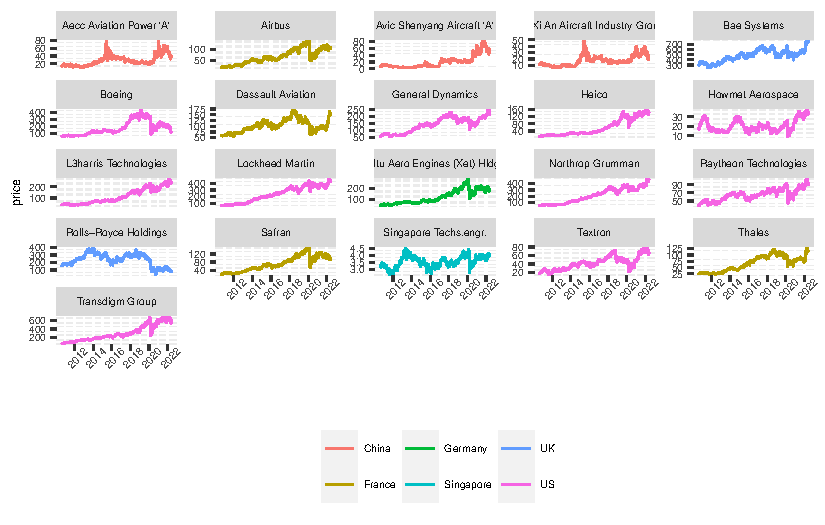
\includegraphics{defence_files/figure-pdf/fig-prices-1.pdf}

}

\caption{\label{fig-prices}Price series levels}

\end{figure}

Figure~\ref{fig-prices} plots the price series levels and highlights
country of incorporation, whereas Figure~\ref{fig-rtns} displays the
log-return series. The price series levels reveal a number of distinct
groupings in their movements. For many cases, price series levels show
common movement with a regime shift towards higher prices and larger
volatility around 2020. Notably, the Chinese stocks experience a shock
in 2016 of similar magnitude to that of 2020. In July 2016 it was
reported that China had performed a week of military drills in the South
China Sea amid legal debates regarding its territorial claims to areas
in the region, which could account for this increase in volatility.
Daily volatility is calculated as the squared of daily log-returns and
presented in Figure~\ref{fig-vols}. Notably, the volatility of some A\&D
companies such as Beoing, Transdigm, Safran, and Rolls-Royce experienced
a spike around the pandemic period and the Russia-Ukraine war.

\begin{figure}[H]

{\centering 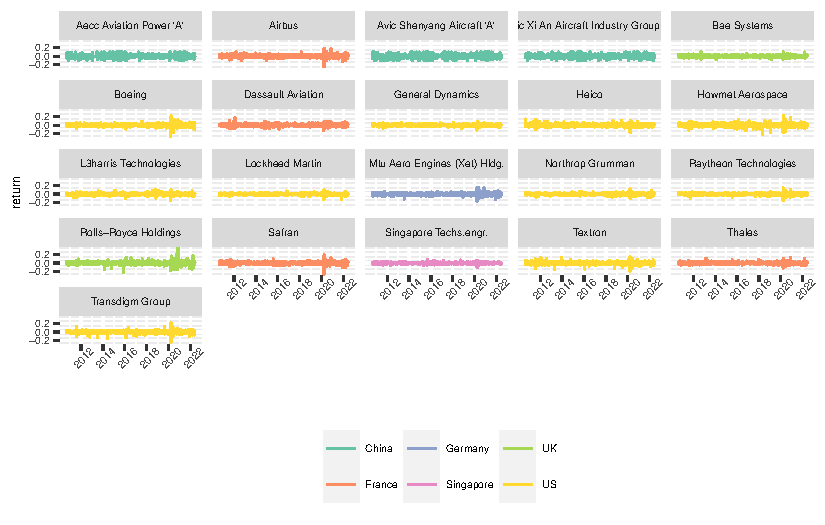
\includegraphics{defence_files/figure-pdf/fig-rtns-1.pdf}

}

\caption{\label{fig-rtns}Daily returns}

\end{figure}

\begin{figure}[H]

{\centering 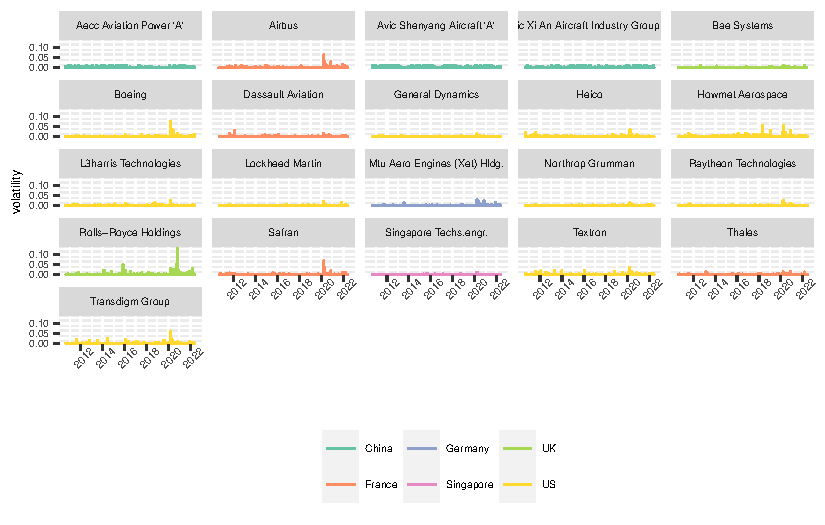
\includegraphics{defence_files/figure-pdf/fig-vols-1.pdf}

}

\caption{\label{fig-vols}Daily Volatilities}

\end{figure}

\hypertarget{tbl-sumrtn}{}
\begin{table}[H]
\caption{\label{tbl-sumrtn}Summary statistics of daily returns }\tabularnewline

\centering
\resizebox{\linewidth}{!}{
\begin{tabular}[t]{lllllllll}
\toprule
A\&D Stock & Mean & Median & Std..Dev. & Skewness & Kurtosis & Jarque.Bera & ADF & PP\\
\midrule
RAYTHEON\_TECHNOLOGIES & 0.0003 & 0.0000 & 0.0157 & -0.3658 & 18.8916 & 32636.5*** & -21.2901*** & -56.4338***\\
LOCKHEED\_MARTIN & 0.0006 & 0.0005 & 0.0132 & -0.7847 & 18.2347 & 30248.2*** & -56.5766*** & -56.7477***\\
BOEING & 0.0003 & 0.0000 & 0.0226 & -0.5643 & 26.2666 & 69973.9*** & -18.1156*** & -52.3339***\\
AIRBUS & 0.0005 & 0.0002 & 0.0222 & -0.3905 & 16.9639 & 25224.5*** & -41.3354*** & -53.1875***\\
NORTHROP\_GRUMMAN & 0.0007 & 0.0005 & 0.0142 & -0.1678 & 10.8567 & 7974.9*** & -57.6092*** & -57.9145***\\
\addlinespace
GENERAL\_DYNAMICS & 0.0004 & 0.0003 & 0.0138 & -0.4154 & 9.2145 & 5069.4*** & -56.0303*** & -56.0601***\\
L3HARRIS\_TECHNOLOGIES & 0.0006 & 0.0004 & 0.0156 & -0.3236 & 13.3721 & 13927.4*** & -37.8971*** & -58.3311***\\
SAFRAN & 0.0005 & 0.0000 & 0.0208 & -0.5873 & 23.2326 & 52968.0 & -27.1859*** & -54.0423***\\
TRANSDIGM\_GROUP & 0.0007 & 0.0006 & 0.0204 & -0.8467 & 26.8661 & 73823.1 & -27.2219*** & -58.6233***\\
BAE\_SYSTEMS & 0.0003 & 0.0000 & 0.0145 & 0.0418 & 7.8111 & 2985.9 & -54.9012*** & -54.8972***\\
\addlinespace
THALES & 0.0005 & 0.0000 & 0.0157 & 0.3395 & 10.4513 & 7219.4 & -52.8929*** & -52.8478***\\
AECC\_AVIATION\_POWER\_\_A\_ & 0.0004 & 0.0000 & 0.0283 & -0.0139 & 6.3355 & 1434.8 & -50.3413*** & -50.2565***\\
HEICO & 0.0009 & 0.0004 & 0.0198 & 0.2280 & 11.1453 & 8582.7 & -37.9681*** & -57.4079***\\
AVIC\_SHENYANG\_AIRCRAFT\_\_A\_ & 0.0007 & 0.0000 & 0.0317 & -0.1037 & 5.3171 & 697.9 & -50.4755*** & -50.432***\\
TEXTRON & 0.0004 & 0.0000 & 0.0215 & -0.3143 & 13.2261 & 13536.4 & -56.7672*** & -56.7572***\\
\addlinespace
HOWMET\_AEROSPACE & 0.0002 & 0.0000 & 0.0250 & -0.3118 & 13.7557 & 14968.7 & -55.6534*** & -55.6534***\\
AVIC\_XI\_AN\_AIRCRAFT\_INDUSTRY\_GROUP\_\_A\_ & 0.0003 & 0.0000 & 0.0274 & -0.1139 & 6.1919 & 1320.5 & -51.6737*** & -51.6765***\\
DASSAULT\_AVIATION & 0.0003 & 0.0000 & 0.0177 & 0.2804 & 10.4996 & 7293.6 & -59.0881*** & -59.3442***\\
MTU\_AERO\_ENGINES\_\_XET\_\_HLDG\_ & 0.0004 & 0.0000 & 0.0196 & -0.2349 & 14.6874 & 17643.4 & -53.5665*** & -53.5378***\\
ROLLS\_ROYCE\_HOLDINGS & -0.0002 & 0.0000 & 0.0263 & 0.8073 & 25.6142 & 66286.0 & -42.2588*** & -53.3912***\\
\addlinespace
SINGAPORE\_TECHS\_ENGR\_ & 0.0001 & 0.0000 & 0.0121 & -0.2655 & 9.6055 & 5663.1 & -58.7849*** & -58.7819***\\
\bottomrule
\end{tabular}}
\end{table}

\hypertarget{tbl-sumvol}{}
\begin{table}[H]
\caption{\label{tbl-sumvol}Summary statistics of daily volatilies }\tabularnewline

\centering
\resizebox{\linewidth}{!}{
\begin{tabular}[t]{lllllllll}
\toprule
A\&D Stock & Mean & Median & Std..Dev. & Skewness & Kurtosis & Jarque.Bera & ADF & PP\\
\midrule
RAYTHEON\_TECHNOLOGIES & 0.0002 & 0.0000 & 0.0010 & 14.3977 & 270.2230 & 9315605 & -8.8644*** & -71.0605***\\
LOCKHEED\_MARTIN & 0.0002 & 0.0000 & 0.0007 & 16.4325 & 350.1678 & 15682053 & -10.8166*** & -57.4850***\\
BOEING & 0.0005 & 0.0001 & 0.0026 & 16.0817 & 339.0628 & 14697726 & -9.4739*** & -59.9743***\\
AIRBUS & 0.0005 & 0.0001 & 0.0020 & 17.2260 & 424.2219 & 23033869 & -11.5572*** & -65.0529***\\
NORTHROP\_GRUMMAN & 0.0002 & 0.0000 & 0.0006 & 11.4526 & 195.7092 & 4856762 & -10.5620*** & -55.0415***\\
\addlinespace
GENERAL\_DYNAMICS & 0.0002 & 0.0000 & 0.0005 & 10.7424 & 180.7454 & 4133764 & -9.4617*** & -64.1503***\\
L3HARRIS\_TECHNOLOGIES & 0.0002 & 0.0001 & 0.0009 & 13.5332 & 273.2503 & 9512974 & -11.8003*** & -53.9115***\\
SAFRAN & 0.0004 & 0.0001 & 0.0020 & 19.3285 & 499.2195 & 31946613 & -11.6048*** & -62.0761***\\
TRANSDIGM\_GROUP & 0.0004 & 0.0001 & 0.0021 & 16.7444 & 377.0165 & 18184391 & -8.6389*** & -55.6789***\\
BAE\_SYSTEMS & 0.0002 & 0.0001 & 0.0006 & 9.3253 & 129.7845 & 2117775 & -16.0119*** & -50.1728***\\
\addlinespace
THALES & 0.0002 & 0.0001 & 0.0008 & 11.6051 & 190.9520 & 4625049 & -16.3795*** & -60.5916***\\
AECC\_AVIATION\_POWER\_\_A\_ & 0.0008 & 0.0001 & 0.0018 & 3.8458 & 18.4539 & 38428 & -9.8441*** & -62.2551***\\
HEICO & 0.0004 & 0.0001 & 0.0013 & 11.4285 & 201.3856 & 5142764 & -9.5040*** & -65.6277***\\
AVIC\_SHENYANG\_AIRCRAFT\_\_A\_ & 0.0010 & 0.0002 & 0.0021 & 3.2338 & 13.5866 & 19848 & -10.2645*** & -62.4013***\\
TEXTRON & 0.0005 & 0.0001 & 0.0016 & 10.1877 & 141.4459 & 2525317 & -10.6989*** & -55.9341***\\
\addlinespace
HOWMET\_AEROSPACE & 0.0006 & 0.0001 & 0.0022 & 13.6603 & 265.6162 & 8990159 & -15.2603*** & -62.3260***\\
AVIC\_XI\_AN\_AIRCRAFT\_INDUSTRY\_GROUP\_\_A\_ & 0.0007 & 0.0002 & 0.0017 & 4.0915 & 21.3110 & 51874 & -10.7828*** & -60.2592***\\
DASSAULT\_AVIATION & 0.0003 & 0.0001 & 0.0010 & 12.8240 & 286.0500 & 10416628 & -12.8417*** & -55.6529***\\
MTU\_AERO\_ENGINES\_\_XET\_\_HLDG\_ & 0.0004 & 0.0001 & 0.0014 & 11.7559 & 179.1791 & 4074035 & -9.3358*** & -66.7664***\\
ROLLS\_ROYCE\_HOLDINGS & 0.0007 & 0.0001 & 0.0034 & 21.7076 & 718.3667 & 66237434 & -5.3944*** & -63.2794***\\
\addlinespace
SINGAPORE\_TECHS\_ENGR\_ & 0.0001 & 0.0000 & 0.0004 & 13.5671 & 279.9223 & 9984241 & -12.0964*** & -67.2677***\\
\bottomrule
\end{tabular}}
\end{table}

Table~\ref{tbl-sumrtn} and Table~\ref{tbl-sumvol} present summary
statistics for daily returns and volatility series, respectively. As
shown in Table~\ref{tbl-sumrtn}, the distributions of the daily returns
series are mostly skewed to the left and exhibit fat ``tailedness'',
with Boeing, Airbus, Rolls-Royce, Safran and Transdigm experiencing the
highest daily volatility. These companies are either directly in the
aviation industry or supply to it, as Rolls-Royce supplies Trent engine
to Airbus. Airlines were hit particularly hard during the COVID-19
pandemic, with an estimated economic loss of US\$168 billion in 2020
(COVID-19's impact on the global aviation sector \textbar{} McKinsey)
which may be a factor in the observed volatility.

Table~\ref{tbl-Xtremes} indicates that most volatile A\&D stock is Rolls
Royce Holdings. The company reported a loss of £4 billion for 2020, and
was forced to raise £7.3 billion in debt and equity and cut almost one
fifth of its workforce (COVID-19: Rolls-Royce blames `severe impact' of
pandemic as it dives to £4bn loss \textbar{} Business News \textbar{}
Sky News). Unsurprisingly Table 2 indicates that the five highest daily
volatility scores mostly occur around the end of March 2020 at the
height of the uncertainty during the onset of the COVID-19 pandemic.

For both return and volatility series, the results of Augmented Dickey
Fuller (ADF) and Phillips-Perron (PP) tests confirm their stationarity
at conventional levels.

\hypertarget{tbl-Xtremes}{}
\begin{table}[H]
\caption{\label{tbl-Xtremes}Extremely votality events }\tabularnewline

\centering
\begin{tabular}[t]{llrrl}
\toprule
Date & stock & return & volatility & country\\
\midrule
2020-03-18 & Airbus & -0.25 & 0.06 & France\\
2020-03-16 & Boeing & -0.27 & 0.07 & US\\
2020-11-09 & Rolls-Royce Holdings & 0.36 & 0.13 & UK\\
2020-03-18 & Safran & -0.26 & 0.07 & France\\
2020-03-18 & Transdigm Group & -0.25 & 0.06 & US\\
\bottomrule
\end{tabular}
\end{table}

\begin{figure}[H]

{\centering 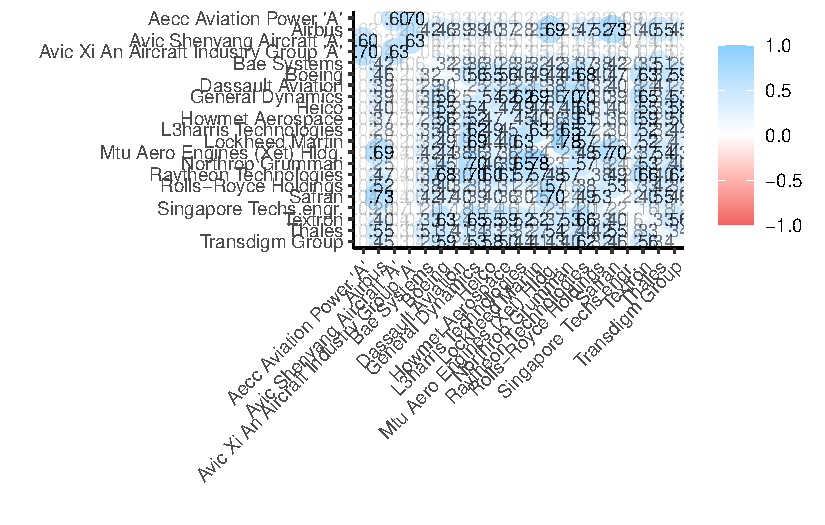
\includegraphics{defence_files/figure-pdf/fig-cor-1.pdf}

}

\caption{\label{fig-cor}Correlation matrix of daily returns}

\end{figure}

Figure~\ref{fig-cor} displays Pearson's pairwise linear correlation
coefficients for the daily returns series. Unsurprisingly, the returns
of many US and European A\&D stocks are highly correlated, for example
between Northrop Grumman and Lockheed Martin. Both firms are leading
suppliers to the US defense department, and regularly win joint
contracts for work. Figure~\ref{fig-cor} also reveals that the Chinese
stocks are highly correlated with each other but uncorrelated with the
firms incorporated in the US and Europe. This corresponds to literature
relating to general stock market trends observed in China, for example
Valukonis (2014) finds that following recovery from the financial crisis
of 2008 Chinese and US stock market indices display weak correlation
which is perhaps due to Chinese markets being somewhat isolated from
global markets and not as influenced by globalization as other markets
may be.

\hypertarget{methodology}{%
\subsection{Methodology}\label{methodology}}

The nature and strength of financial market linkages has traditionally
been measured using conventional mean estimators. Ando, Greenwood-Nimmo,
and Shin (2022) argue that systemic shocks are likely to be much larger
than average shocks and that it need not be the case that large shocks
propagate in the same way as smaller shocks. Therefore using
quantile-based estimators can identify whether the topology of the
network of spillovers changes with the size of the shocks that affect
the system. To study the return and volatility connectedness across 21
global defence and aerospace firms, we use the quantile-VAR-based
connectedness approach introduced by {[}Ando, Greenwood-Nimmo, and Shin
(2022){]}\footnote{The methodology has been used by Bouri et al.~(2020),
  Chatziantoniou et al.~(2021) and Saeed et al.~(2021).}. This approach
extends the mean-based connectedness framework (Diebold and Yilmaz 2009;
Diebold and Yılmaz 2014) and thus allows for capturing extreme
connectedness measures estimated at the lower, middle, and upper
quantiles. For returns, this allows for capturing the connectedness of
return shocks in bear, normal, and bull periods. For volatility, we
capture connectedness of volatility shocks in low, middle, and high
volatility states.

We consider a portfolio enivroment, where stocks are indexed
i=1,2,\ldots,N, and time periods are indexed t=1,2,\ldots,T. Based on a
quantile regression (Koenker, 2005), we consider a quantile-VAR process
of p\textsuperscript{th} order for a set of N return (volatility) series
for time T, \(y_{it}=\{y_{t=1,i=1},\dots,y_{t=T,i=N}\}\) , as given by:

\[
y_{t}=c_{i(\tau)}+\sum_{j=1}^{p} B_{j,(\tau)} y_{t-j}+e_{t(\tau)}, t=1,\dots,T
\]

where, \(c_{(\tau)}\) denotes a vector of constant terms at quantile τ,
\(B_{j(\tau)}\) represents the matrix of the j\textsuperscript{th}
lagged coefficients of the dependent variable at quantile τ, with i
=1,\ldots, p, and \(e_{t(\tau)}\) denotes a vector of error terms at
quantile τ. Equation (1) is estimated by assuming that the error terms
conform to the population quantile restriction,
\(Q_t(e_{t(\tau)} |y_{t=1},\dots,y_{t=p})=0\) .

We express the τth conditional quantile of response y as:

\[
Q_t(y_t |y_{t=1},\dots,y_{t=p})=c_{(\tau)}+\hat{B_{i(\tau)}} y_{t-i}
\]

Following the approach of Diebold and Yılmaz (2014) , we compute return
and volatility connectedness measures based on a quantile variance
decomposition.

We represent Equation
\href{https://www.sciencedirect.com/science/article/pii/S1062940819304085\#e0015}{(3)}
as an infinite order vector moving average process:

\[
y_t=\mu_{(\tau)}+\sum_{s=0}^{\infty}A_{s(\tau)}e_{t-s(\tau)}, t=1,\dots.T
\]

where,

\begin{align*}
\mu{(\tau)}= \frac{c_{\tau}}{\left (I_n-B_{1(\tau)}-\dots-B_{p(\tau)} \right)} \\
A_{s(\tau)}= \begin{cases} 0, s<0 \\ I_n, s=0 \\ B_{1(\tau)}A_{s-1(\tau)}+\dots+B_{p(\tau)}A_{s-p(\tau)}, s>0 \end{cases} \\
\text{and $y_t$ is given by the sum of $e_{t(\tau)}$}
\end{align*}

The generalized forecast error variance decomposition
(GFEVD),\(\theta^h_{i,j}\), is computed as in Diebold and Yılmaz (2014).
The GFEVD reflects the contribution of the i\textsuperscript{th} stock
return (volatility) to the variance of the forecast error of the stock
return (volatility) i\textsuperscript{th} at h-steps ahead and is
defined as:

\[
\theta^{(h)}_{j \leftarrow i,(\tau)}= \frac{\sigma_{ii}^{-1}\sum_{l=0}^{h}(e_j^{'}h_h \Omega_{(\tau)} e_j)^2}{\sum_{h=0}^{H-1}(e_i^{'}h_h \Omega_{(\tau)} e_i)}
\]

where, V is the variance matrix of the vector of residuals,
\(\sigma_{ii}\) is the j\textsuperscript{th} diagonal element of the V
matrix, and \(e_i\)denotes a vector with a value of 1 for the
i\textsuperscript{th} element and 0 otherwise.

Its scaled version,\(\theta_{j\leftarrow i,(\tau)}^h\) , is represented
as:

\[
\theta_{j\leftarrow i,(\tau)}^h=\frac{\theta^{(h)}_{j \leftarrow i,(\tau)}}{\sum_{j=1}^N \theta^{(h)}_{j \leftarrow i,(\tau)}}
\]

The scaled version measures the spillover of the idiosyncratic shock
affecting variable i onto variable j (Ando, Greenwood-Nimmo, and Shin
2022).

Various spillover measures are estimated at each quantile and are
summaries in Table 2

\begin{longtable}[]{@{}
  >{\raggedright\arraybackslash}p{(\columnwidth - 4\tabcolsep) * \real{0.2361}}
  >{\raggedright\arraybackslash}p{(\columnwidth - 4\tabcolsep) * \real{0.2917}}
  >{\raggedright\arraybackslash}p{(\columnwidth - 4\tabcolsep) * \real{0.4722}}@{}}
\caption{Table 1: Description of modelling outputs}\tabularnewline
\toprule\noalign{}
\begin{minipage}[b]{\linewidth}\raggedright
Name
\end{minipage} & \begin{minipage}[b]{\linewidth}\raggedright
Formula
\end{minipage} & \begin{minipage}[b]{\linewidth}\raggedright
Description
\end{minipage} \\
\midrule\noalign{}
\endfirsthead
\toprule\noalign{}
\begin{minipage}[b]{\linewidth}\raggedright
Name
\end{minipage} & \begin{minipage}[b]{\linewidth}\raggedright
Formula
\end{minipage} & \begin{minipage}[b]{\linewidth}\raggedright
Description
\end{minipage} \\
\midrule\noalign{}
\endhead
\bottomrule\noalign{}
\endlastfoot
Own share &
\(                                                                                                                                                                                                                                                                                                                                                                                                                                                                                                                                                                                                                                                                                                                                                                                                                                                                                                                                                                                                                                                                                                                                                                                                                                                                                                                                        
                                                                                                                                                                                                                                                                                                                                                                                                                                                                                                                                                                                                                                                                                                                                                                                                                                                                                                                                                                                                                                                                                                              \tilde{\theta_{j\leftarrow i,(\tau)}^h}                                                                                                                                                                                                   
                                                                                                                                                                                                                                                                                                                                                                                                                                                                                                                                                                                                                                                                                                                                                                                                                                                                                                                                                                                                                                                                                                              \)
& The proportion of the h-steps-ahead GFECD of the ith variable that can
be attributed to the shocks to variable i \\
FROM &
\(                                                                                                                                                                                                                                                                                                                                                                                                                                                                                                                                                                                                                                                                                                                                                                                                                                                                                                                                                                                                                                                                                                                                                                                                                                                                                                                                        
                                                                                                                                                                                                                                                                                                                                                                                                                                                                                                                                                                                                                                                                                                                                                                                                                                                                                                                                                                                                                                                                                                              F_{i \leftarrow \cdot,(\tau)}^h =\sum_{j=1,i \ne j}^m \theta_{j\leftarrow i,(\tau)}^h                                                                                                                                                     
                                                                                                                                                                                                                                                                                                                                                                                                                                                                                                                                                                                                                                                                                                                                                                                                                                                                                                                                                                                                                                                                                                              \)
& Measures the total spillover from the system to i, capturing external
condition effects on i. \\
TO &
\(                                                                                                                                                                                                                                                                                                                                                                                                                                                                                                                                                                                                                                                                                                                                                                                                                                                                                                                                                                                                                                                                                                                                                                                                                                                                                                                                        
                                                                                                                                                                                                                                                                                                                                                                                                                                                                                                                                                                                                                                                                                                                                                                                                                                                                                                                                                                                                                                                                                                              T_{\cdot \leftarrow i,(\tau)}^h =\sum_{j=1,i \ne j}^m \theta_{j\leftarrow i,(\tau)}^h                                                                                                                                                     
                                                                                                                                                                                                                                                                                                                                                                                                                                                                                                                                                                                                                                                                                                                                                                                                                                                                                                                                                                                                                                                                                                              \)
& Measures the total spillover from i to the system, capturing the
influence of ith node in the network. \\
NET &
\(                                                                                                                                                                                                                                                                                                                                                                                                                                                                                                                                                                                                                                                                                                                                                                                                                                                                                                                                                                                                                                                                                                                                                                                                                                                                                                                                        
                                                                                                                                                                                                                                                                                                                                                                                                                                                                                                                                                                                                                                                                                                                                                                                                                                                                                                                                                                                                                                                                                                              T_{\cdot \leftarrow i,(\tau)}^h -F_{i \leftarrow \cdot,(\tau)}^h                                                                                                                                                                          
                                                                                                                                                                                                                                                                                                                                                                                                                                                                                                                                                                                                                                                                                                                                                                                                                                                                                                                                                                                                                                                                                                              \)
& Meaures the directional connectedness of variable i. \\
TOTAL &
\(                                                                                                                                                                                                                                                                                                                                                                                                                                                                                                                                                                                                                                                                                                                                                                                                                                                                                                                                                                                                                                                                                                                                                                                                                                                                                                                                        
                                                                                                                                                                                                                                                                                                                                                                                                                                                                                                                                                                                                                                                                                                                                                                                                                                                                                                                                                                                                                                                                                                              S_{\tau}^h=m^{-1}\sum                                                                                                                                                                                                                     
                                                                                                                                                                                                                                                                                                                                                                                                                                                                                                                                                                                                                                                                                                                                                                                                                                                                                                                                                                                                                                                                                                              F_{i \leftarrow \cdot,(\tau)}^h                                                                                                                                                                                                           
                                                                                                                                                                                                                                                                                                                                                                                                                                                                                                                                                                                                                                                                                                                                                                                                                                                                                                                                                                                                                                                                                                              \)
& Is the sum of the from system estimates. \\
\end{longtable}

Table 1 describes the modelling output measurements. The third column
describes how these can be interpreted in terms of their network
dynamics. Note that, by construction, \texttt{own\ share} and
\texttt{FROM} sum to one for i=1,2,..,m, buy \texttt{TO} can take values
greater than or less than one.

The lag order of the quantile VARs is selected based on SIC. It is equal
to 1 for the quantile-VAR of return series and 2 for the quantile-VAR of
volatility series. As for the forecast horizon (H), we use 10 days.
Furthermore, we conduct a time-varying spillover analysis (Diebold and
Yilmaz (2014) based on a rolling window of 200 days. To assess the
robustness of our results, we use a fixed window length of 200 days and
a 5-step forecast horizon and show that our spillover results remain
almost the same, suggesting their robustness to the window size and
forecast horizon. These results are not reported here but are available
on request from the authors. (If needed, I can add these results to
Appendix).

\hypertarget{results}{%
\section{Results}\label{results}}

In the context of global defense stocks, we are mostly interested in the
nature of network dynamics due to crisis periods and conflict events,
which is particularly relevant in the current geopolitical climate. In
terms of financial risk management the propagation of idiosyncratic risk
contagion is often defined in relation to the difference in the way that
the shock propagates during extreme events relative to normal times
(Londono 2019). Our analysis thus attempts to investigate how much of
the uncertainty associated with stock can be attributed to the
idiosyncratic shocks coming from stock as the shock size varies.

We present both the return and volatility spillovers across A\&D stocks
under study. The sample period includes both normal and extreme market
conditions, including the Russia-Ukraine war.

\hypertarget{network-topology-of-return-and-volatility-spillovers}{%
\subsection{Network topology of return and volatility
spillovers}\label{network-topology-of-return-and-volatility-spillovers}}

To understand the aggregate spillover intensity among our defence and
aerospace stocks we use visualise the results of a full-sample analysis
for both returns and volatility at the median, 5th and 95th percentile.
These network visualisation represent the strength of the bilateral
spillovers by relative thickness of the edges, while the size of each
node is proportional to the square root of the total spillover (inwards
and outwards) (Ando, Greenwood-Nimmo, and Shin 2022). Finally, the
country of origin of the company is represented by colour.

\hypertarget{return-spillovers}{%
\subsubsection{Return spillovers}\label{return-spillovers}}

Figures 5 - 7 illustrate the network visualization of the static
bilateral spillover effects of the 21 return series, while Figures 8 -
Figure 10 display the same visualization for the volatility series. Some
similar patterns emerge, notably the consistent size of the US stock
nodes representing the large aggregate spillover effects in both
directions. Raytheon Technology in all plots experiences the largest
aggregate spillover effects, indicative of its dominance in the A\&D
industry. However, there are also some important differences. Firstly,
the strongest individual pairwise spillover effects are observed at the
median conditional distribution, mostly within countries. Notably,
Chinese stocks show the strongest linkages within country but the
weakest linkages outside their country of origin, consistent with
earlier discussions. In contrast, at the extremes of the return
distribution, all pairwise spillover effects are weaker. This finding is
consistent with previous studies, which show that in times of stress the
network is characterized by a larger number of weaker bilateral linkages
resulting in an increase in the weight completeness of the network
(Dungey, Harvey, and Volkov 2019; Ando, Greenwood-Nimmo, and Shin 2022).
In our context, this would mean that while shocks spillovers between
individual stocks pairs are small, the overall connectedness of the
network is increasing in times of stress, meaning that the shock
propagation is higher under extreme return conditions.

\begin{figure}[H]

{\centering 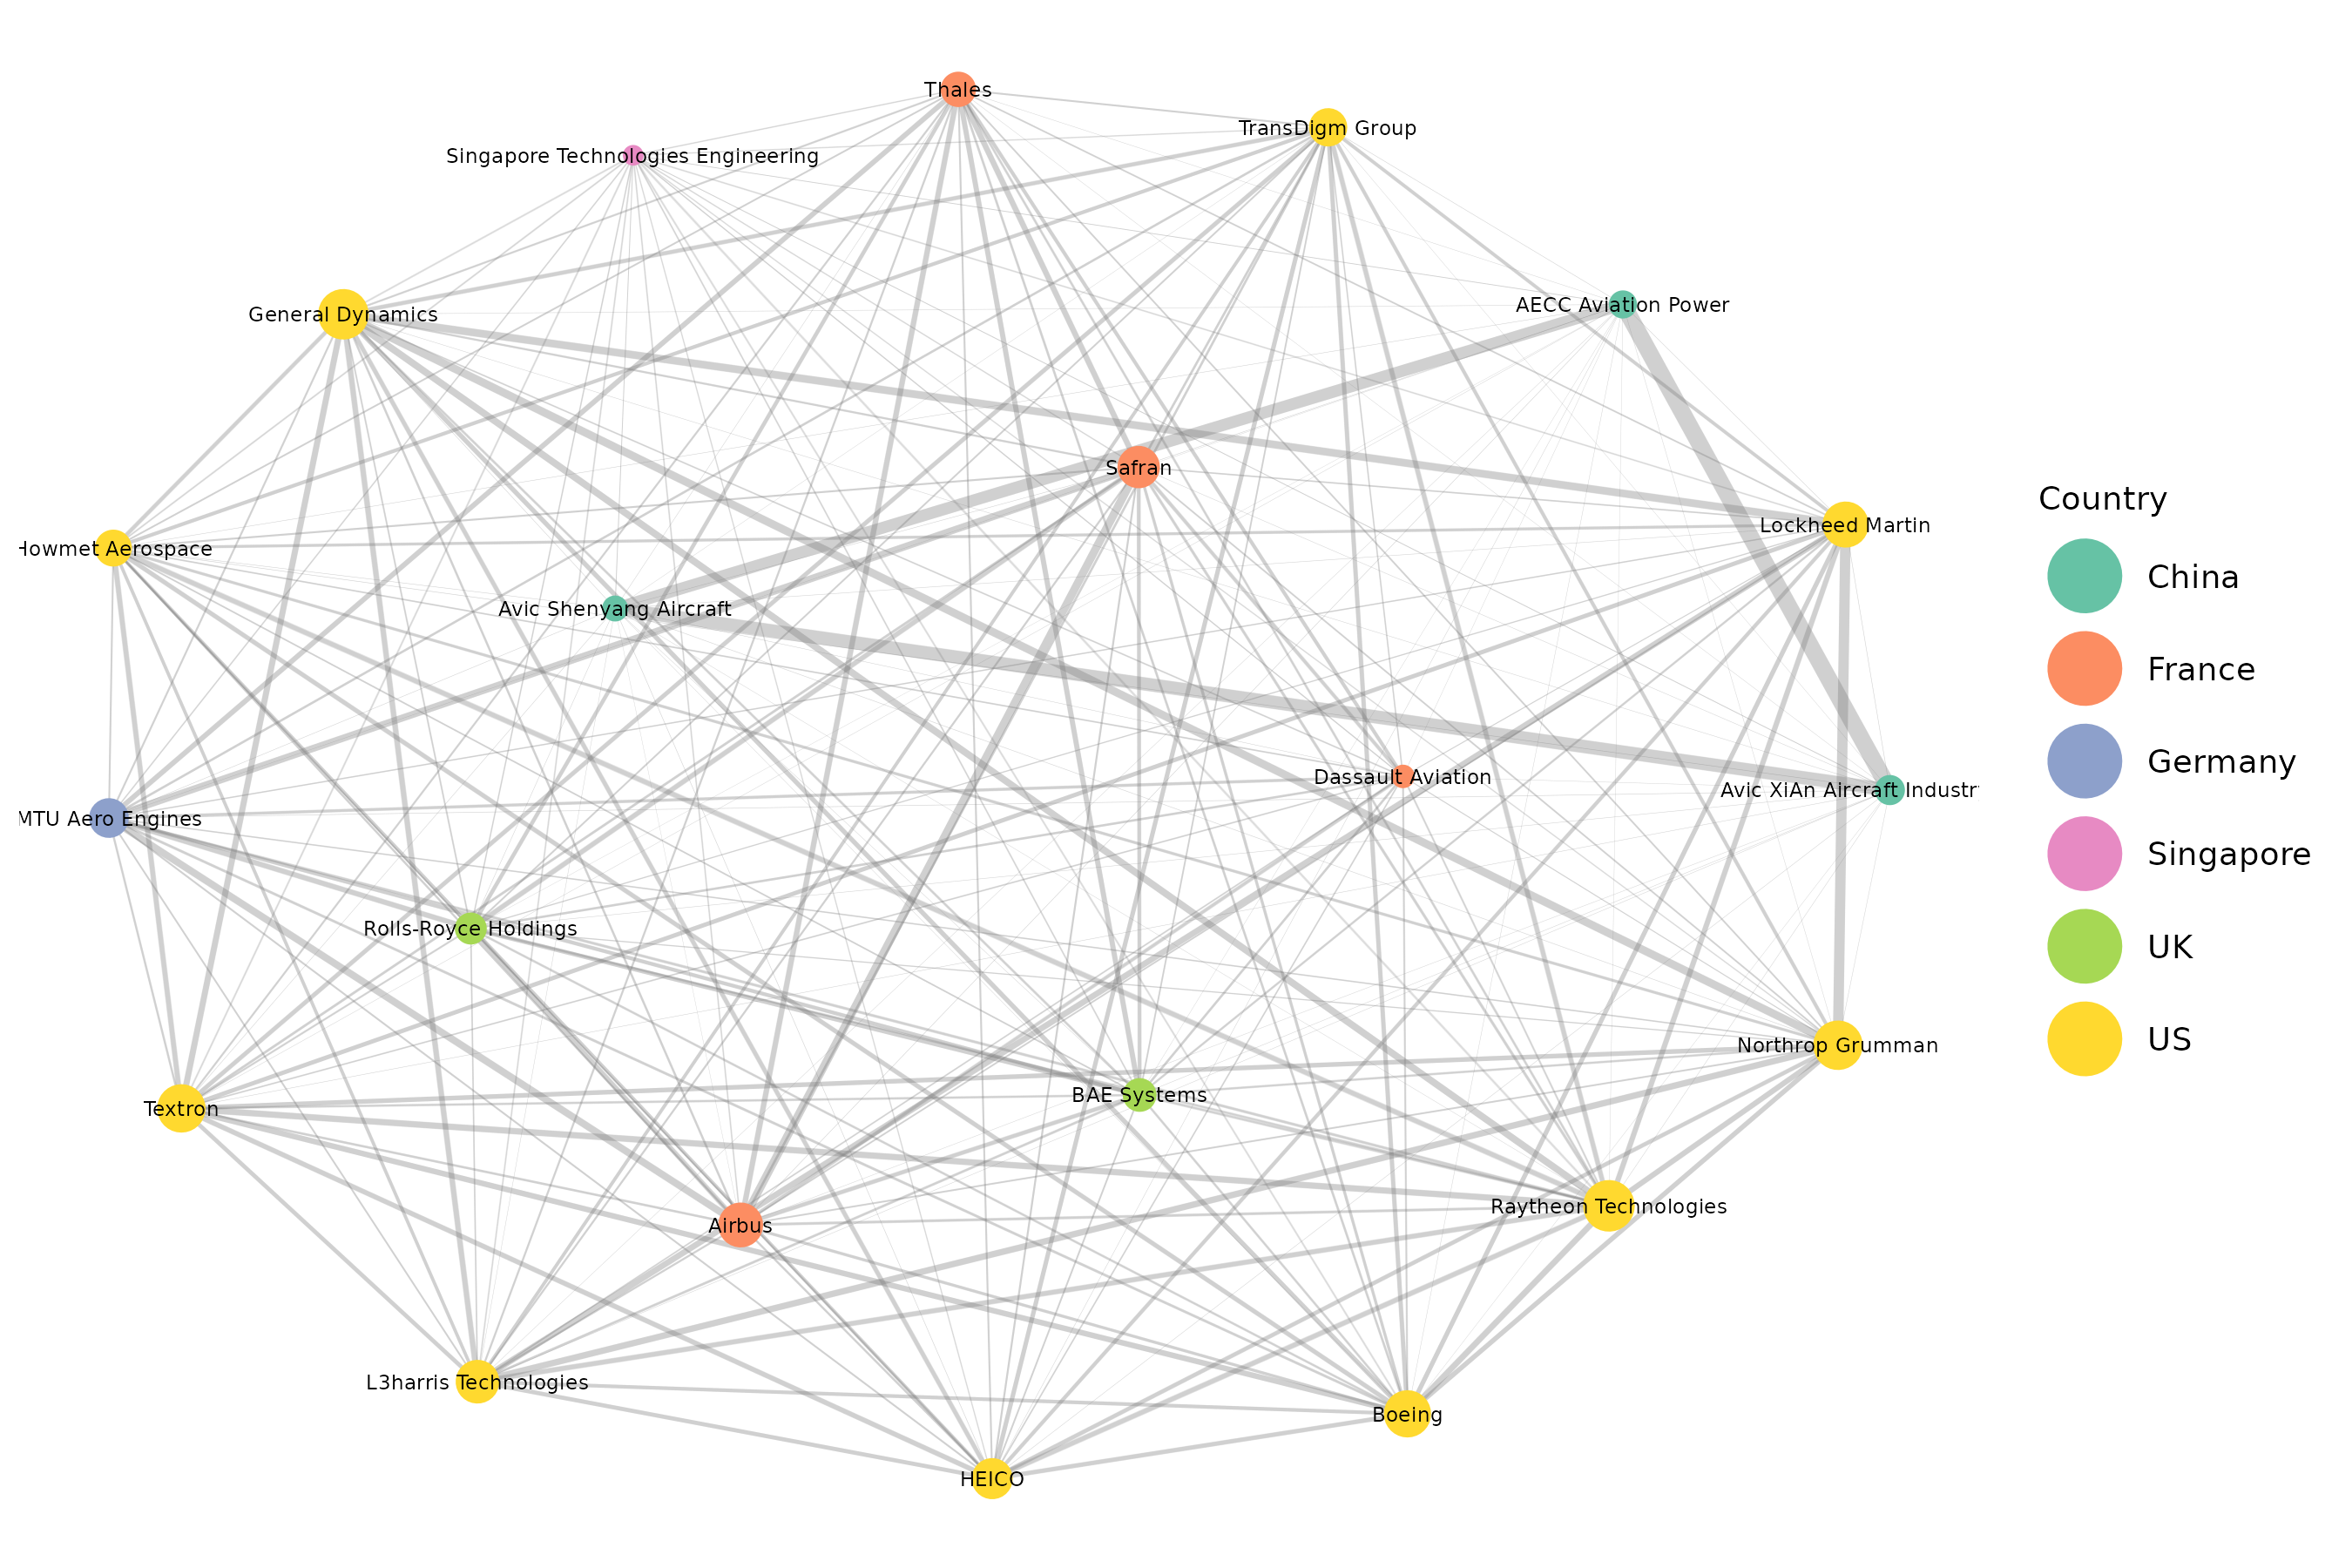
\includegraphics[width=6.75in,height=\textheight]{plots/fig-rtn50.png}

}

\caption{\label{fig-rtn50}Network topology of static results for returns
at the 50th percentile}

\end{figure}

\begin{figure}[H]

{\centering 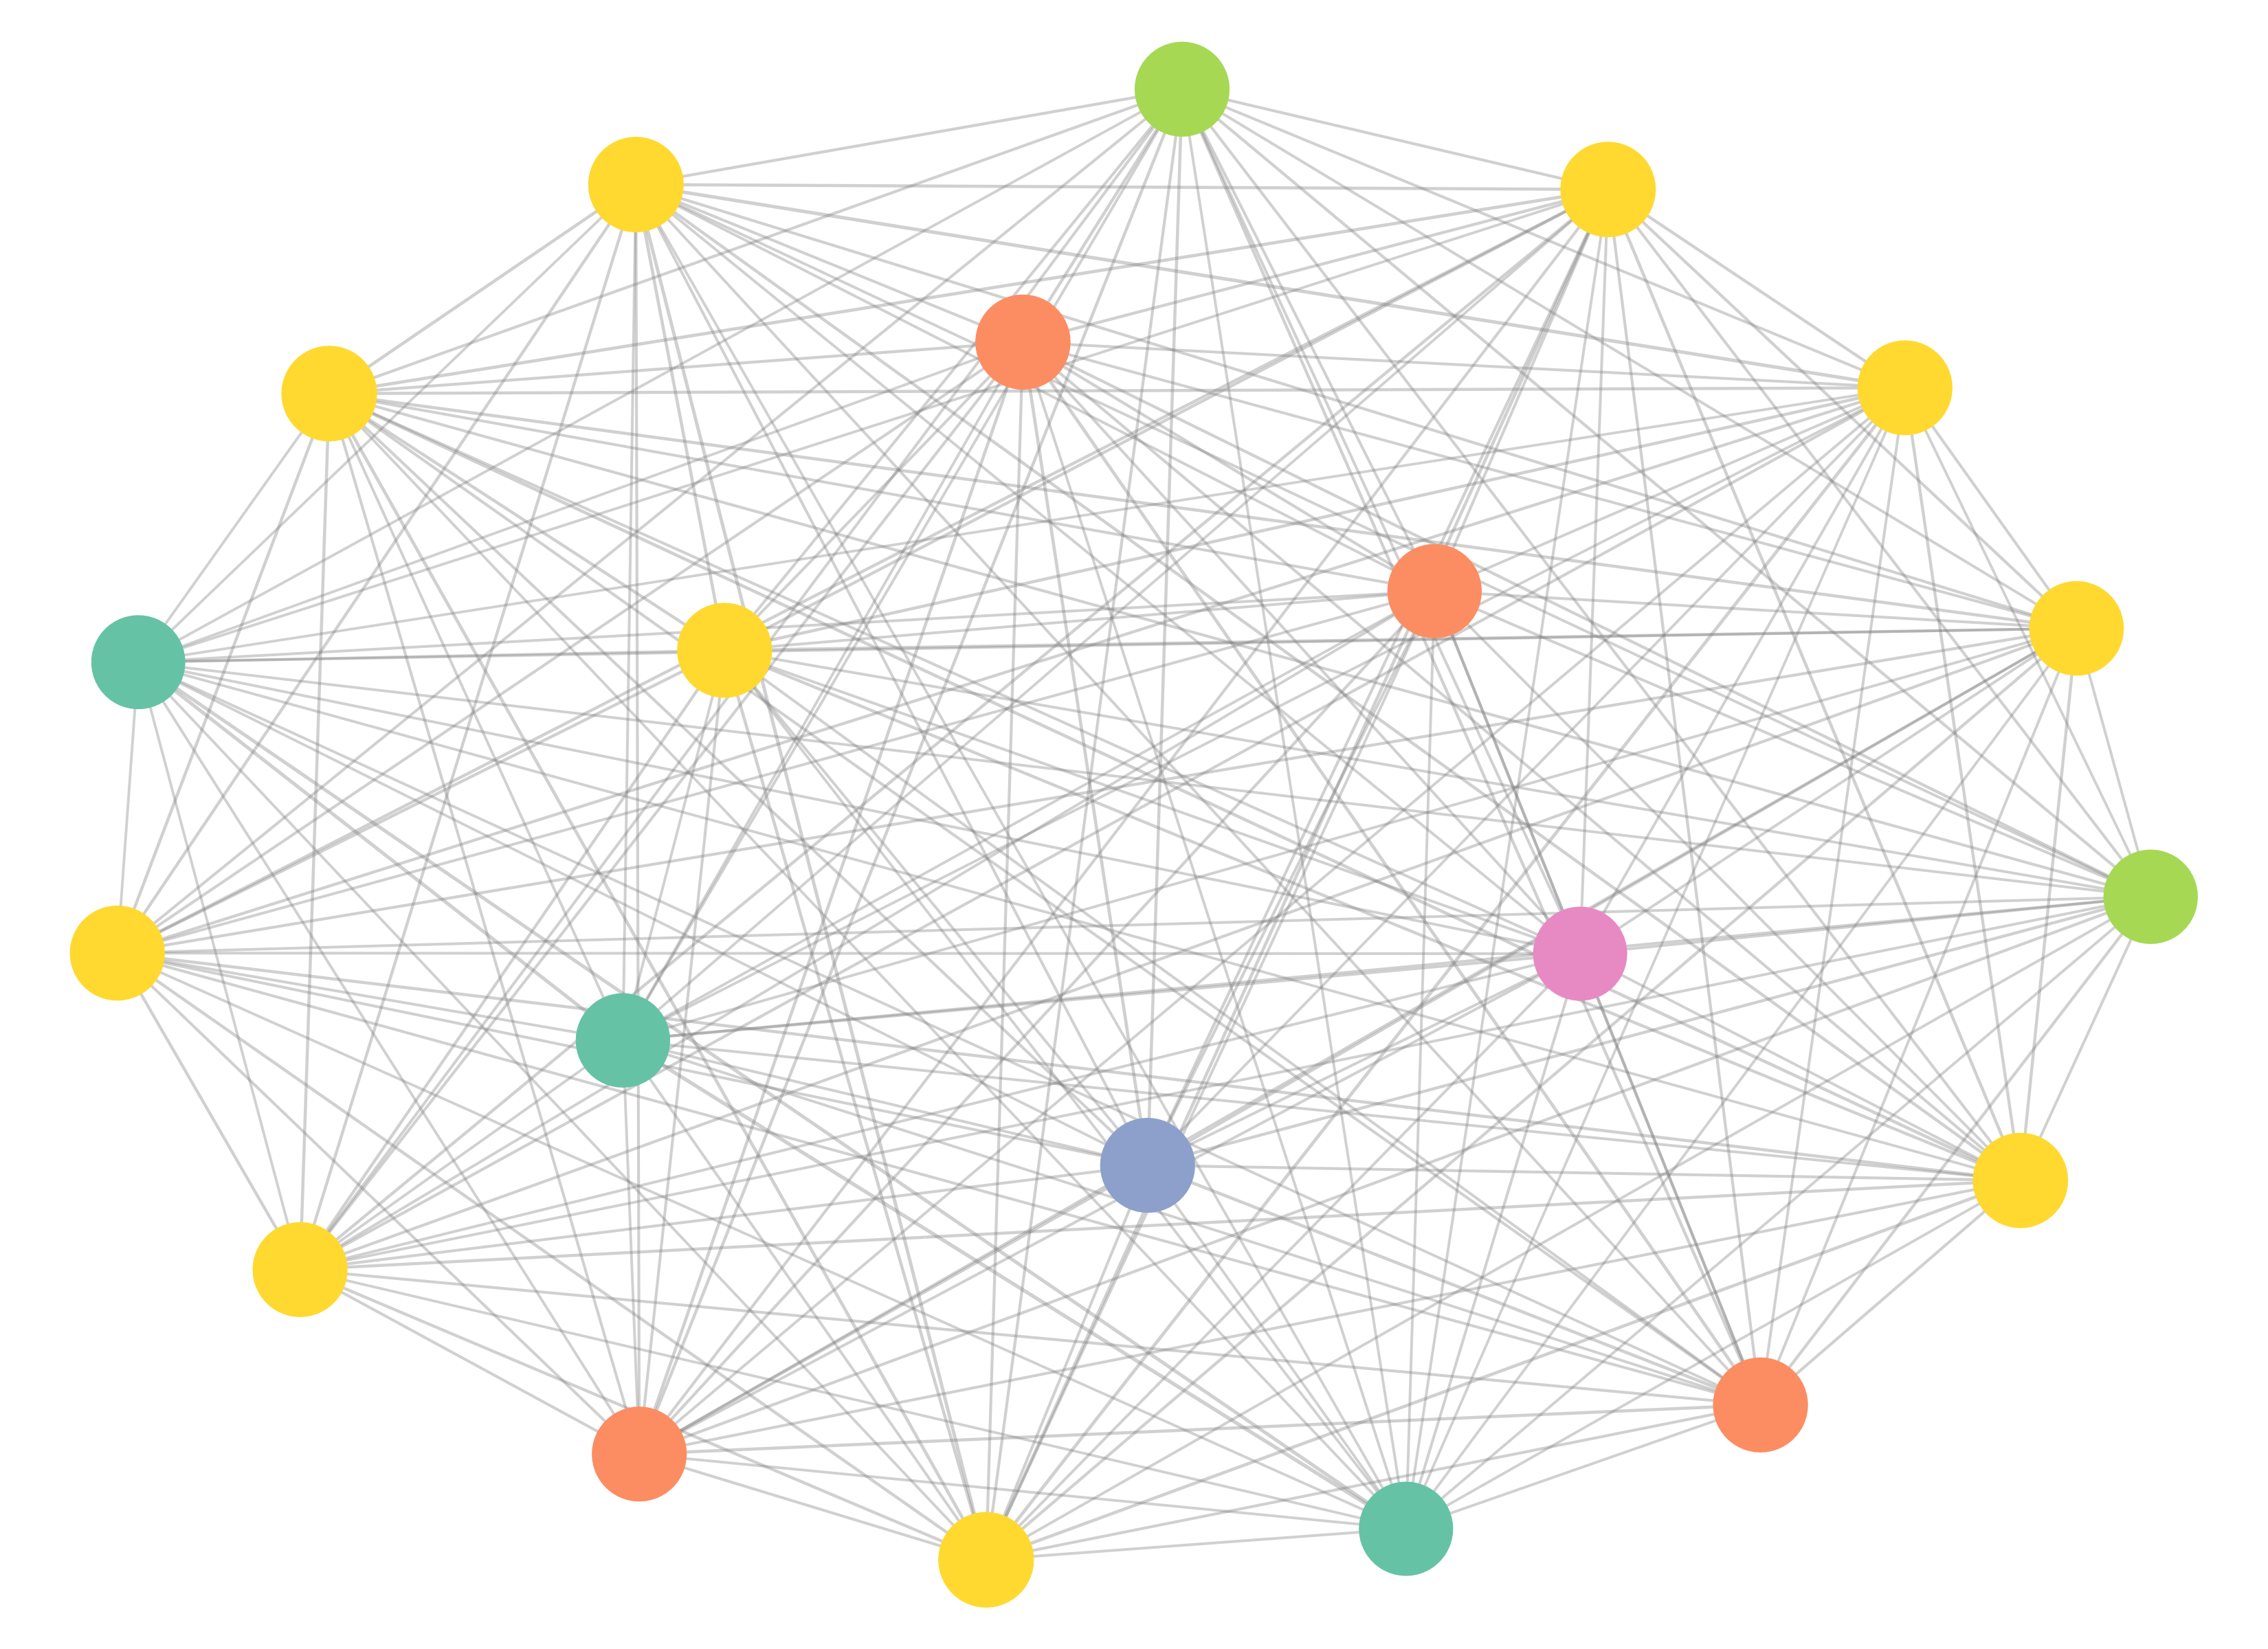
\includegraphics[width=6.75in,height=\textheight]{plots/fig-rtn95.png}

}

\caption{\label{fig-rtn95}Network topology of static results for returns
at the 95th percentile}

\end{figure}

\begin{figure}[H]

{\centering 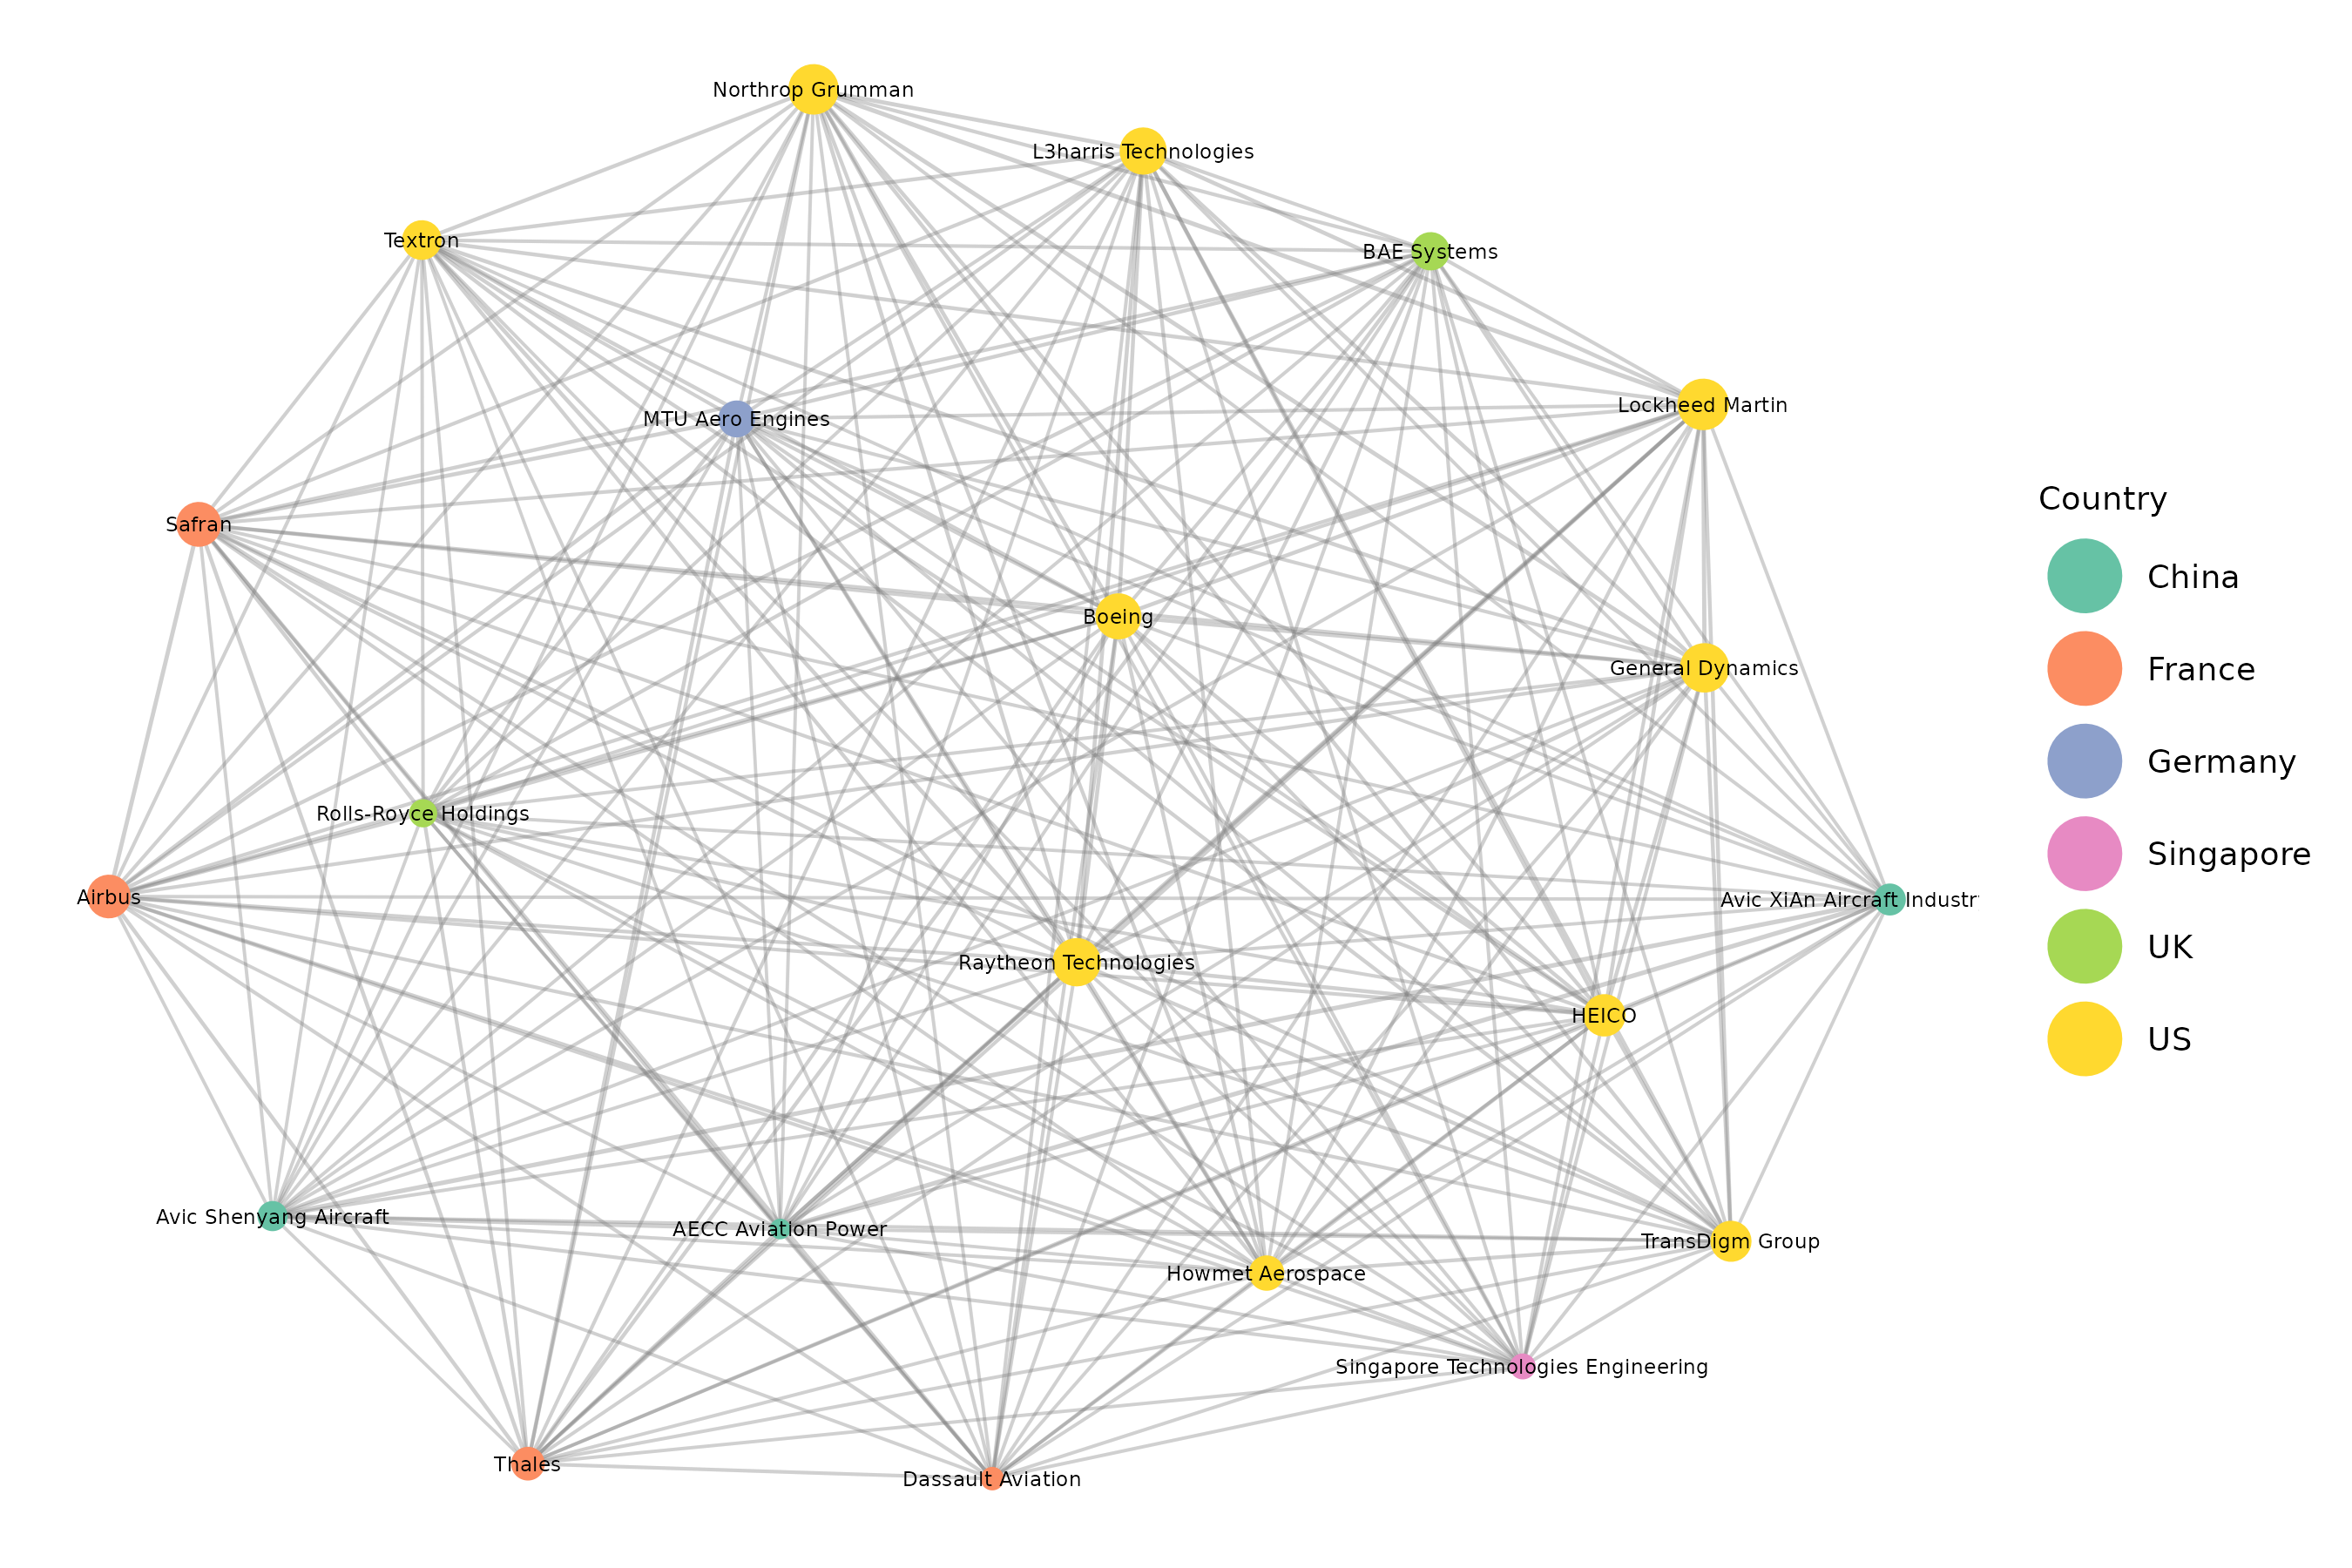
\includegraphics[width=6.75in,height=\textheight]{plots/fig-rtn5.png}

}

\caption{\label{fig-rtn5}Network topology of static results for returns
at the 5th percentile}

\end{figure}

\hypertarget{volatility-spillovers}{%
\subsubsection{Volatility spillovers}\label{volatility-spillovers}}

Moving to the network of volatility spillovers, Figures 8-10 exhibit a
similar pattern to those for the return spillovers in that the extreme
upper quantile is characterized by weak bilateral spillovers and the
strongest pairwise spillovers occur at the median quantile. Here we
again observe the strongest linkages between Chinese countries, followed
by linkages between US companies. Strong linkages between Chinese
companies are also apparent at the extreme lower quantile. Huang et al.
(2021) construct a tail risk spillover network for China's industry
sectors. The national defense sector is defined as a `downstream' sector
due to its position in the industrial chain and it is found that it has
relatively high volatility compared to other leading industries. Bu,
Tang, and Wu (2019) analyse movement in the Chinese stock market using a
causal network method, finding that in normal period investors are
concerned with risk and return but in crisis periods they are only
concerned about risk.

\begin{figure}[H]

{\centering 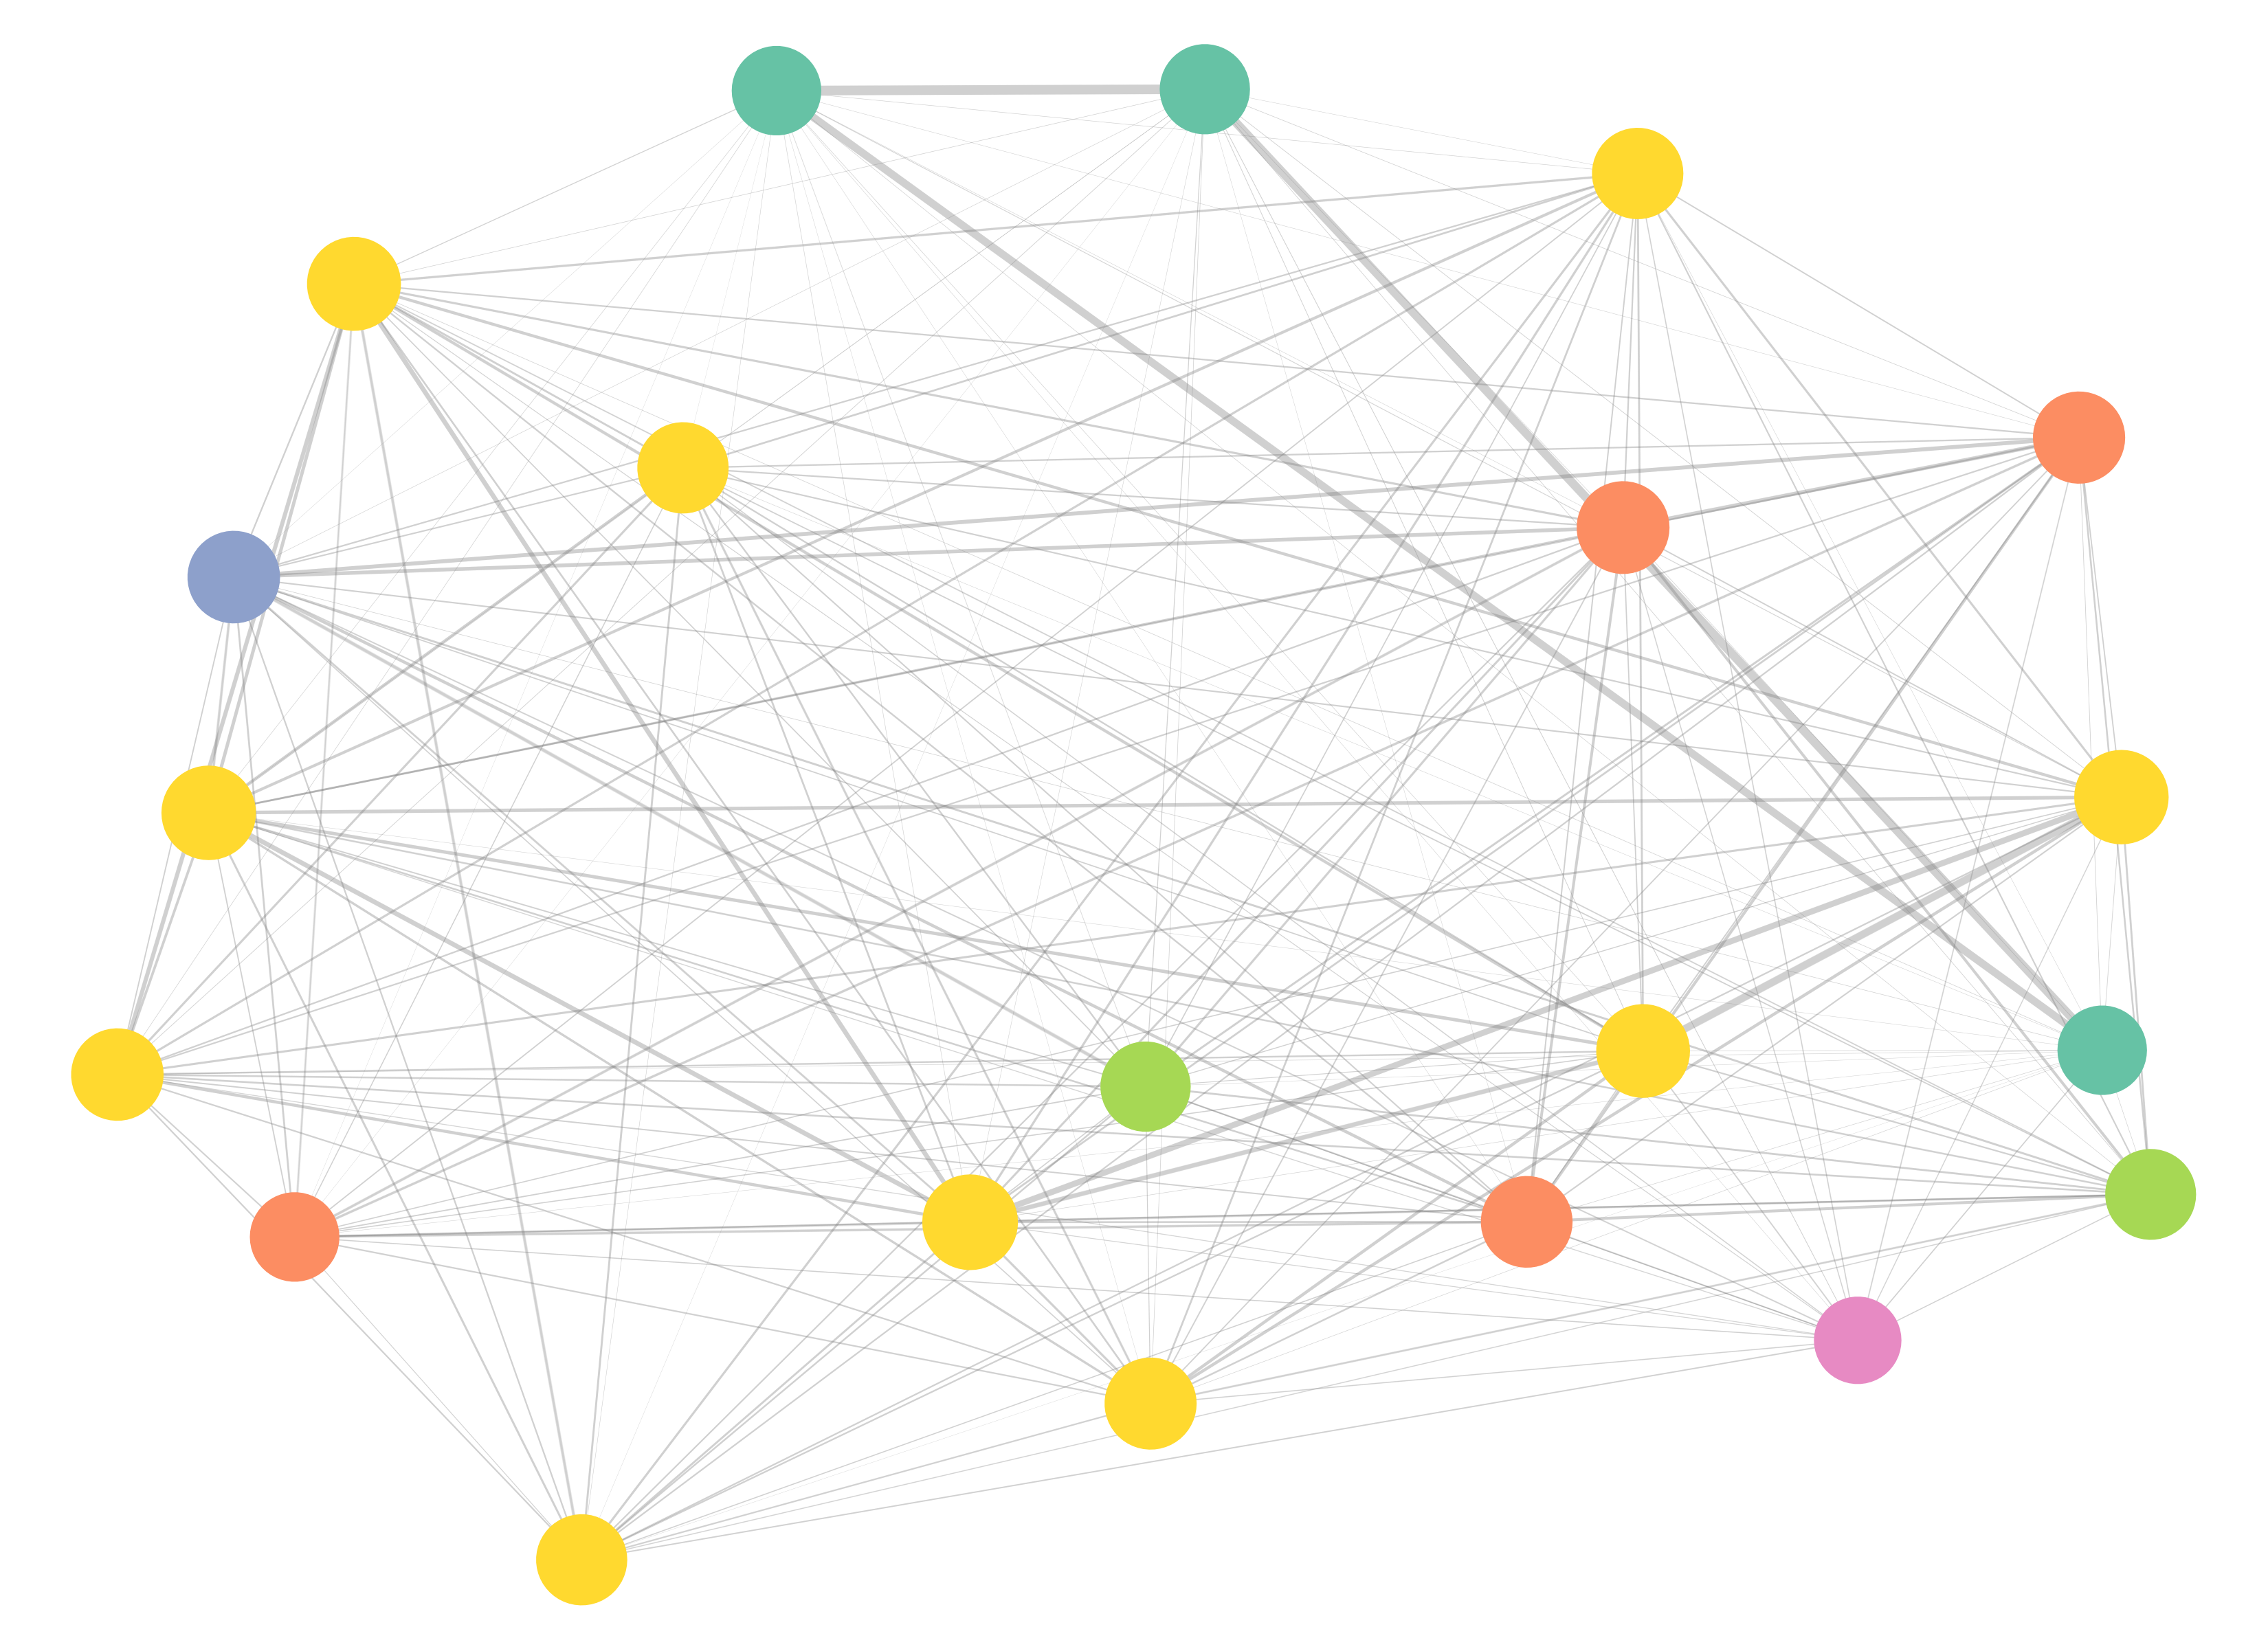
\includegraphics[width=6.75in,height=\textheight]{plots/fig-vol50.png}

}

\caption{\label{fig-vol50}Network topology of static results for
volatility at the 50th percentile}

\end{figure}

\begin{figure}[H]

{\centering 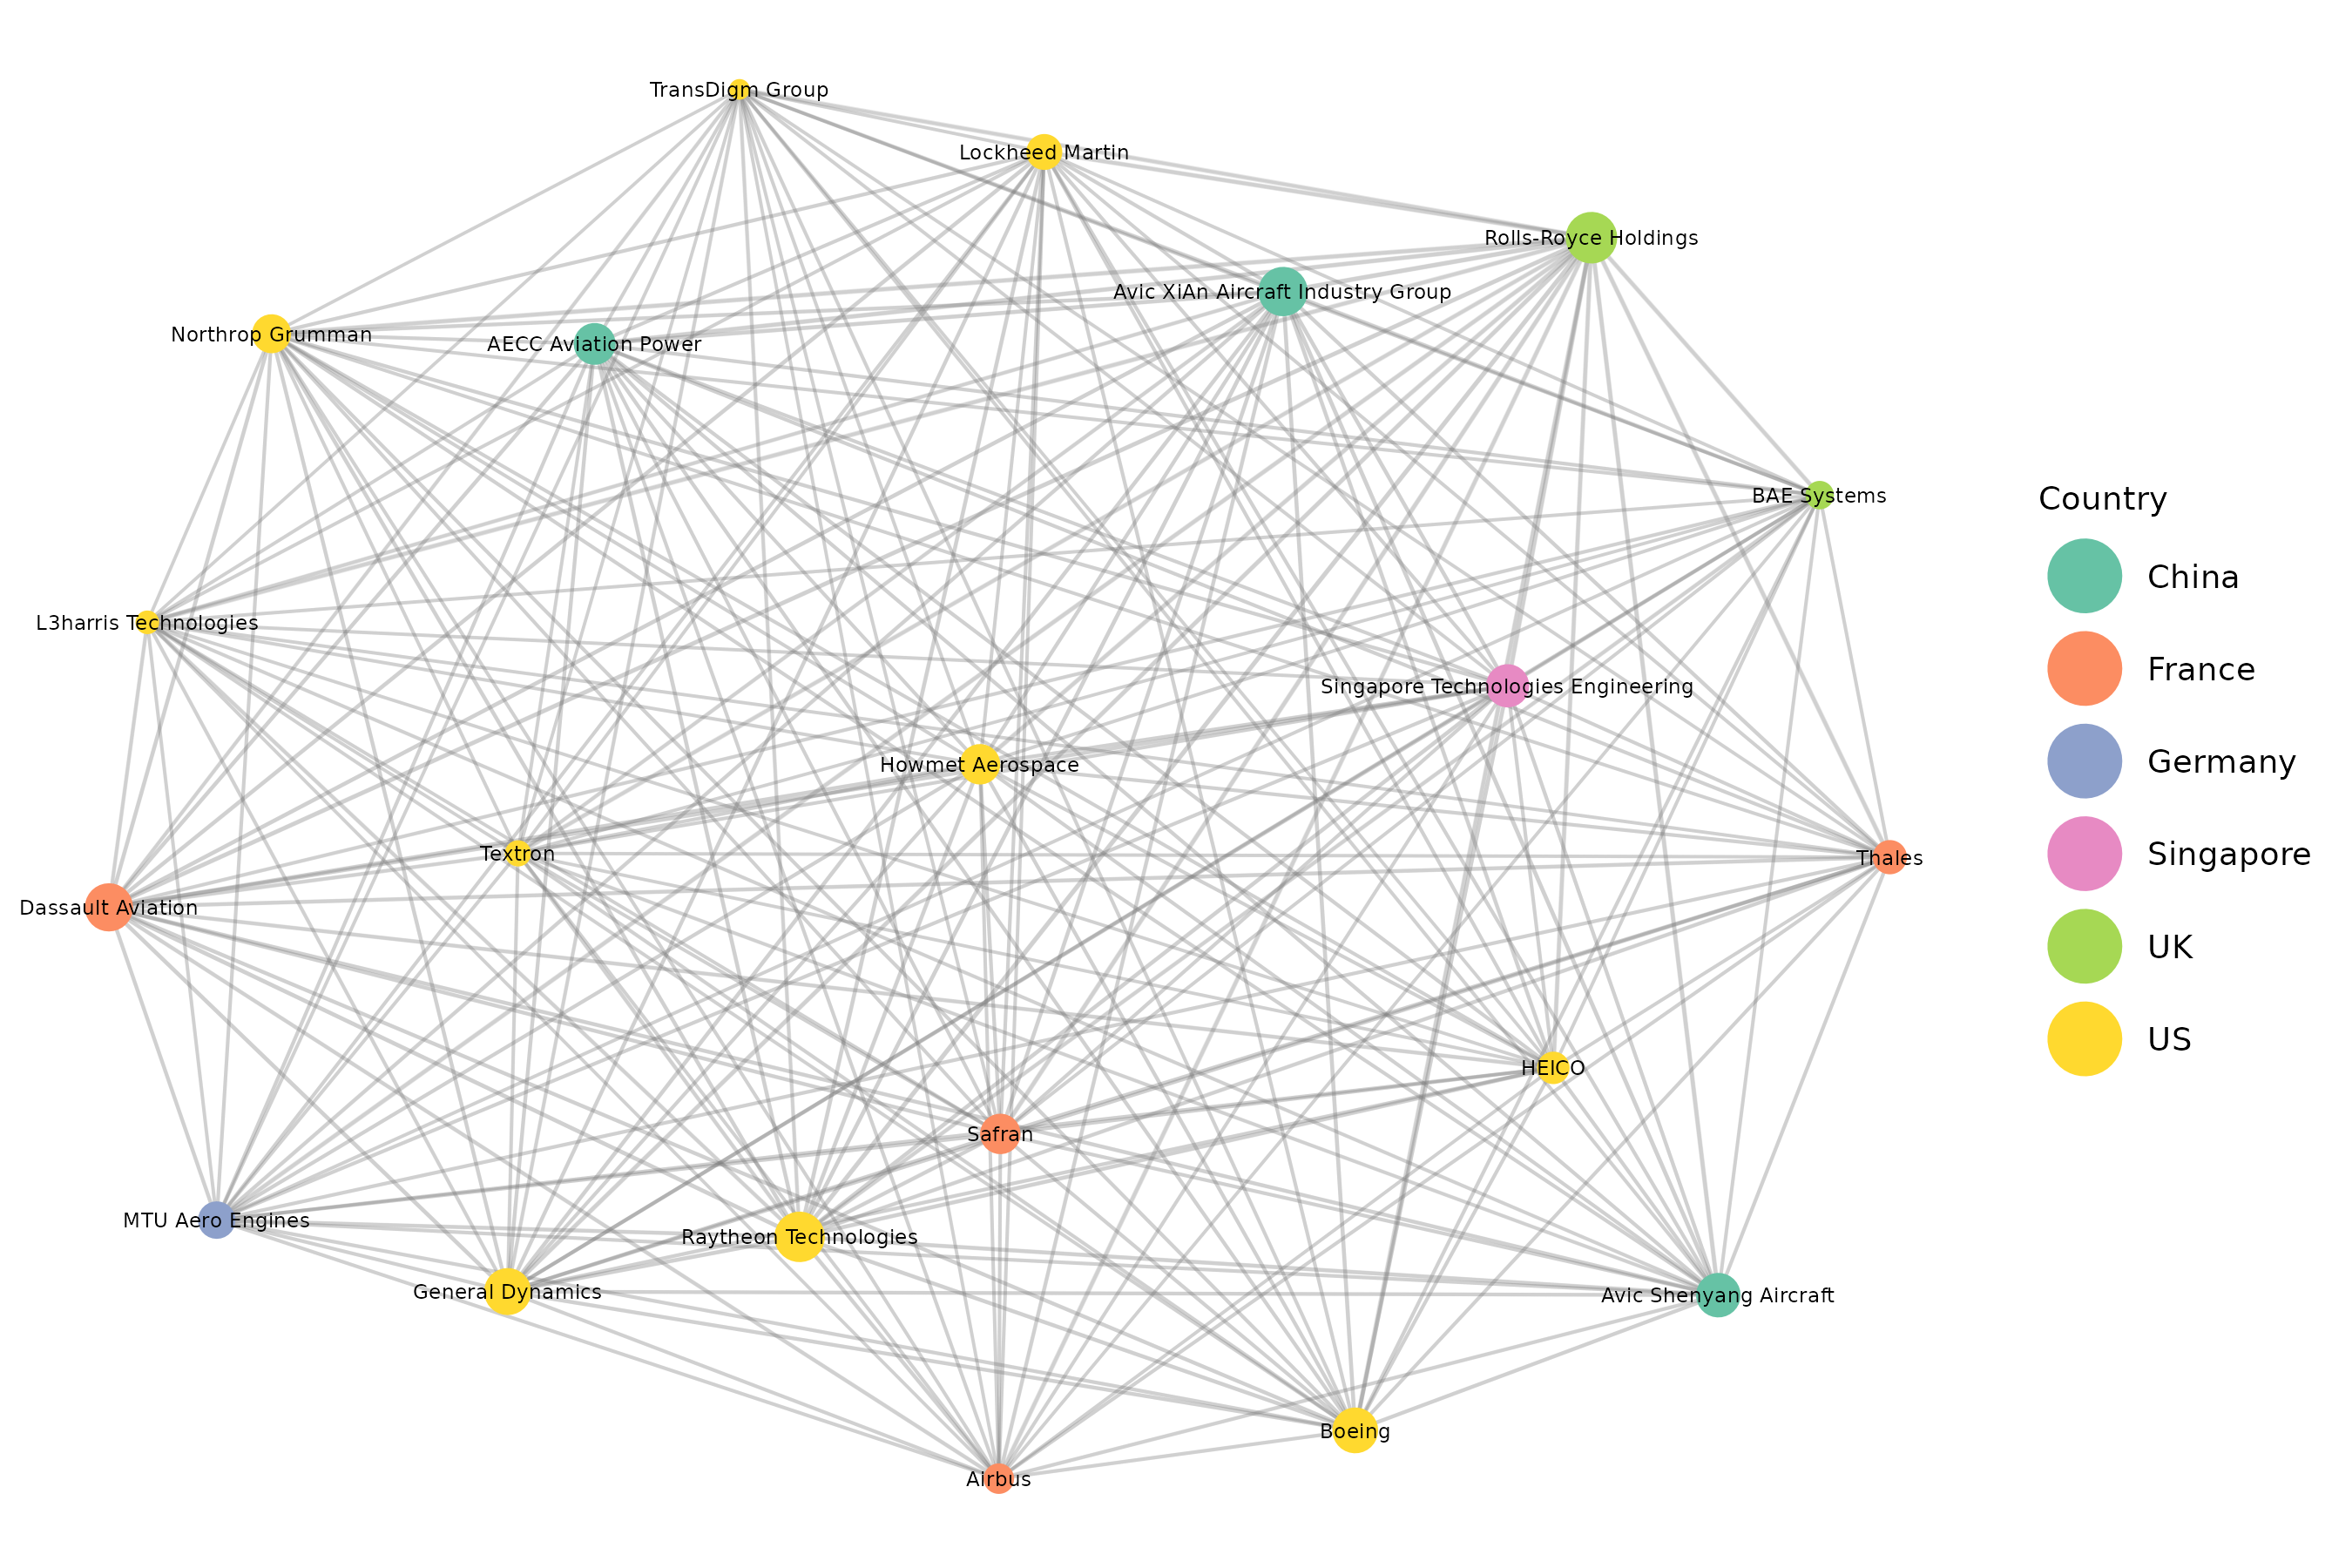
\includegraphics[width=6.75in,height=\textheight]{plots/fig-vol95.png}

}

\caption{\label{fig-vol95}Network topology of static results for
volatility at the 95th percentile}

\end{figure}

\begin{figure}[H]

{\centering 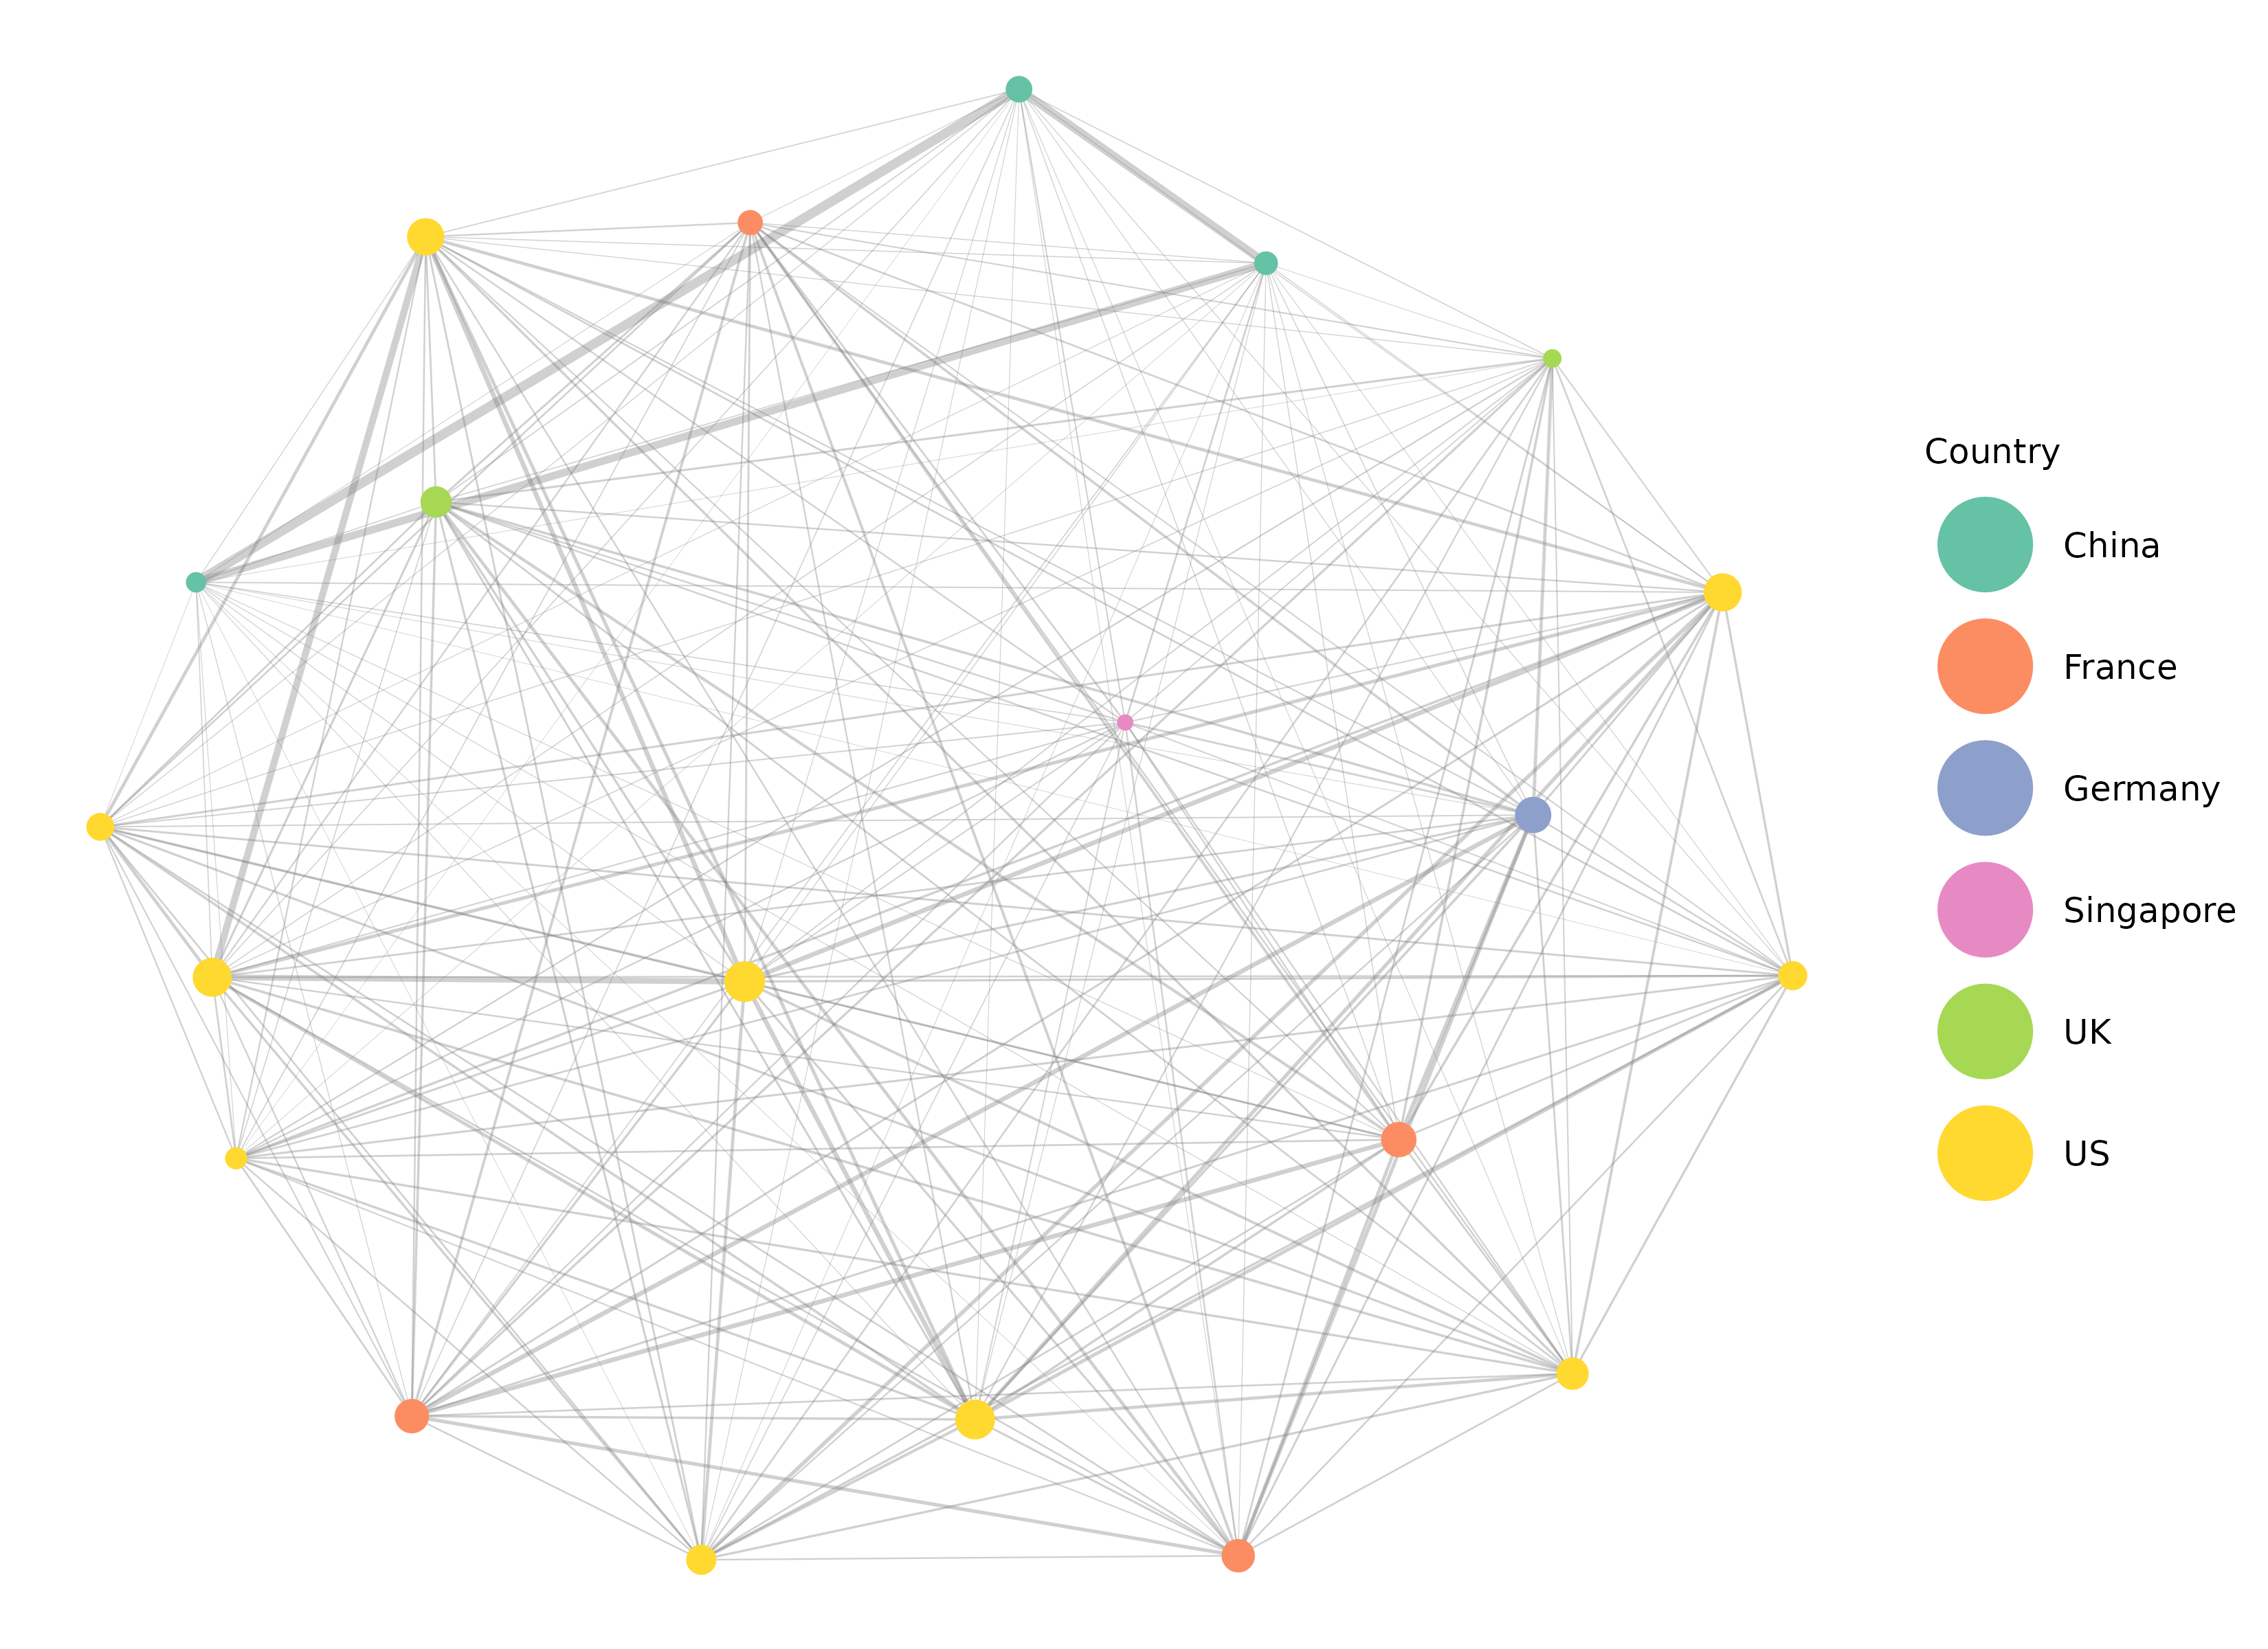
\includegraphics[width=6.75in,height=\textheight]{plots/fig-vol5.png}

}

\caption{\label{fig-vol5}Network topology of static results for
volatility at the 5th percentile}

\end{figure}

\hypertarget{time-varying-spillover-results}{%
\subsection{Time varying spillover
results}\label{time-varying-spillover-results}}

So far, we have analysed measures of connectedness for the entire sample
using static network topology visualisation. However, it is important to
illustrate meaningful time variation in the topology of both returns and
volatility networks of defense stocks under various market conditions.
Furthermore, we find that bilateral spillover of idiosyntractic risk are
stronger for both returns and volatility systems of defense stocks,
which reflect the interconnectedness across A\&D stocks. However, it is
important to note that restricting the network analysis to the middle of
the distribution with this static approach will fail to capture the full
extent of dependence when large shocks occur (i.e.~under extreme market
conditions and events). Therefore in this section, we conduct a rolling
analysis with a quantile VAR to capture the time variability in the
return spillovers in normal times (i.e.~the median of the conditional
distribution) and abnormal market conditions (i.e.~the upper and lower
tails of the conditional distribution). We use a fixed window length of
200\footnote{Existing studies in the Deibold-Yilmaz network literature
  use windows ranging from 100-250 days. Sensitivity analysis has been
  done and available upon request.} days and a 10-step forecast horizon.
This will provide a comprehensive analysis of connectedness at the
center and in the left and right tail dependence. This is conducted for
both returns and volatility.

\hypertarget{total-system-connectivity}{%
\subsubsection{Total system
connectivity}\label{total-system-connectivity}}

\begin{figure}[H]

{\centering 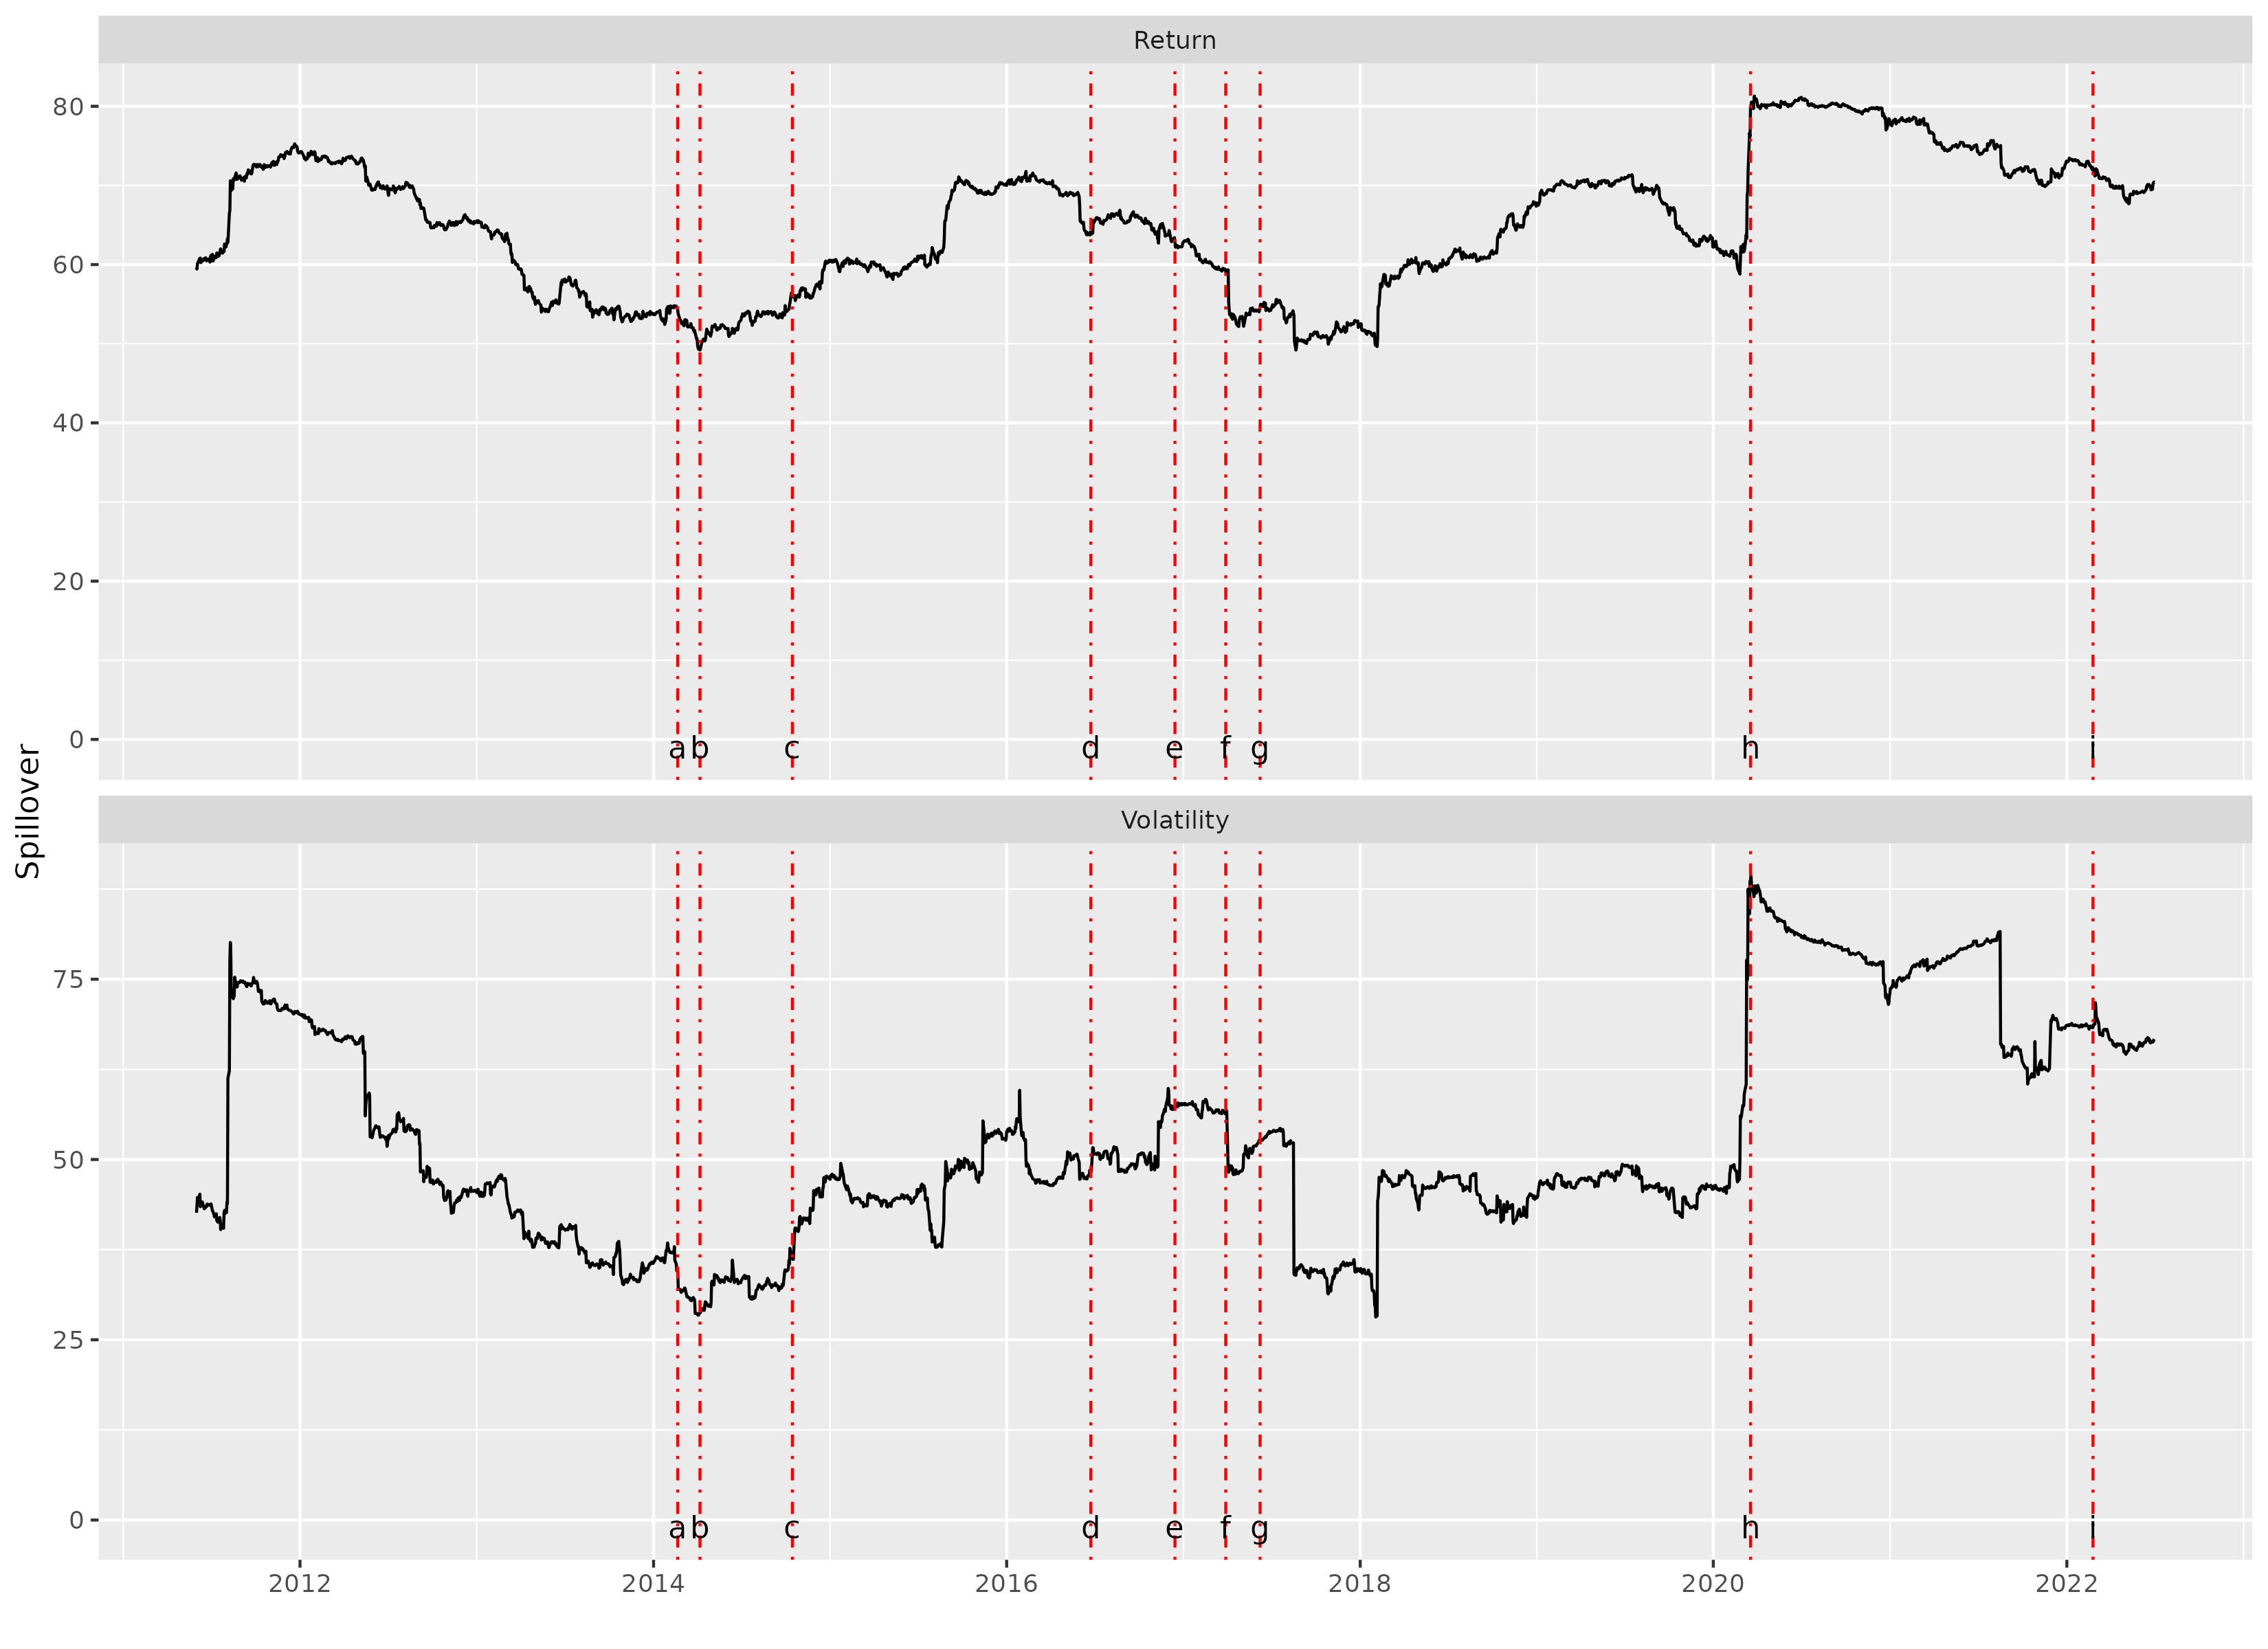
\includegraphics{plots/fig-TCI50.png}

}

\caption{\label{fig-TCI50}Conditional Median}

\end{figure}

\begin{figure}[H]

{\centering 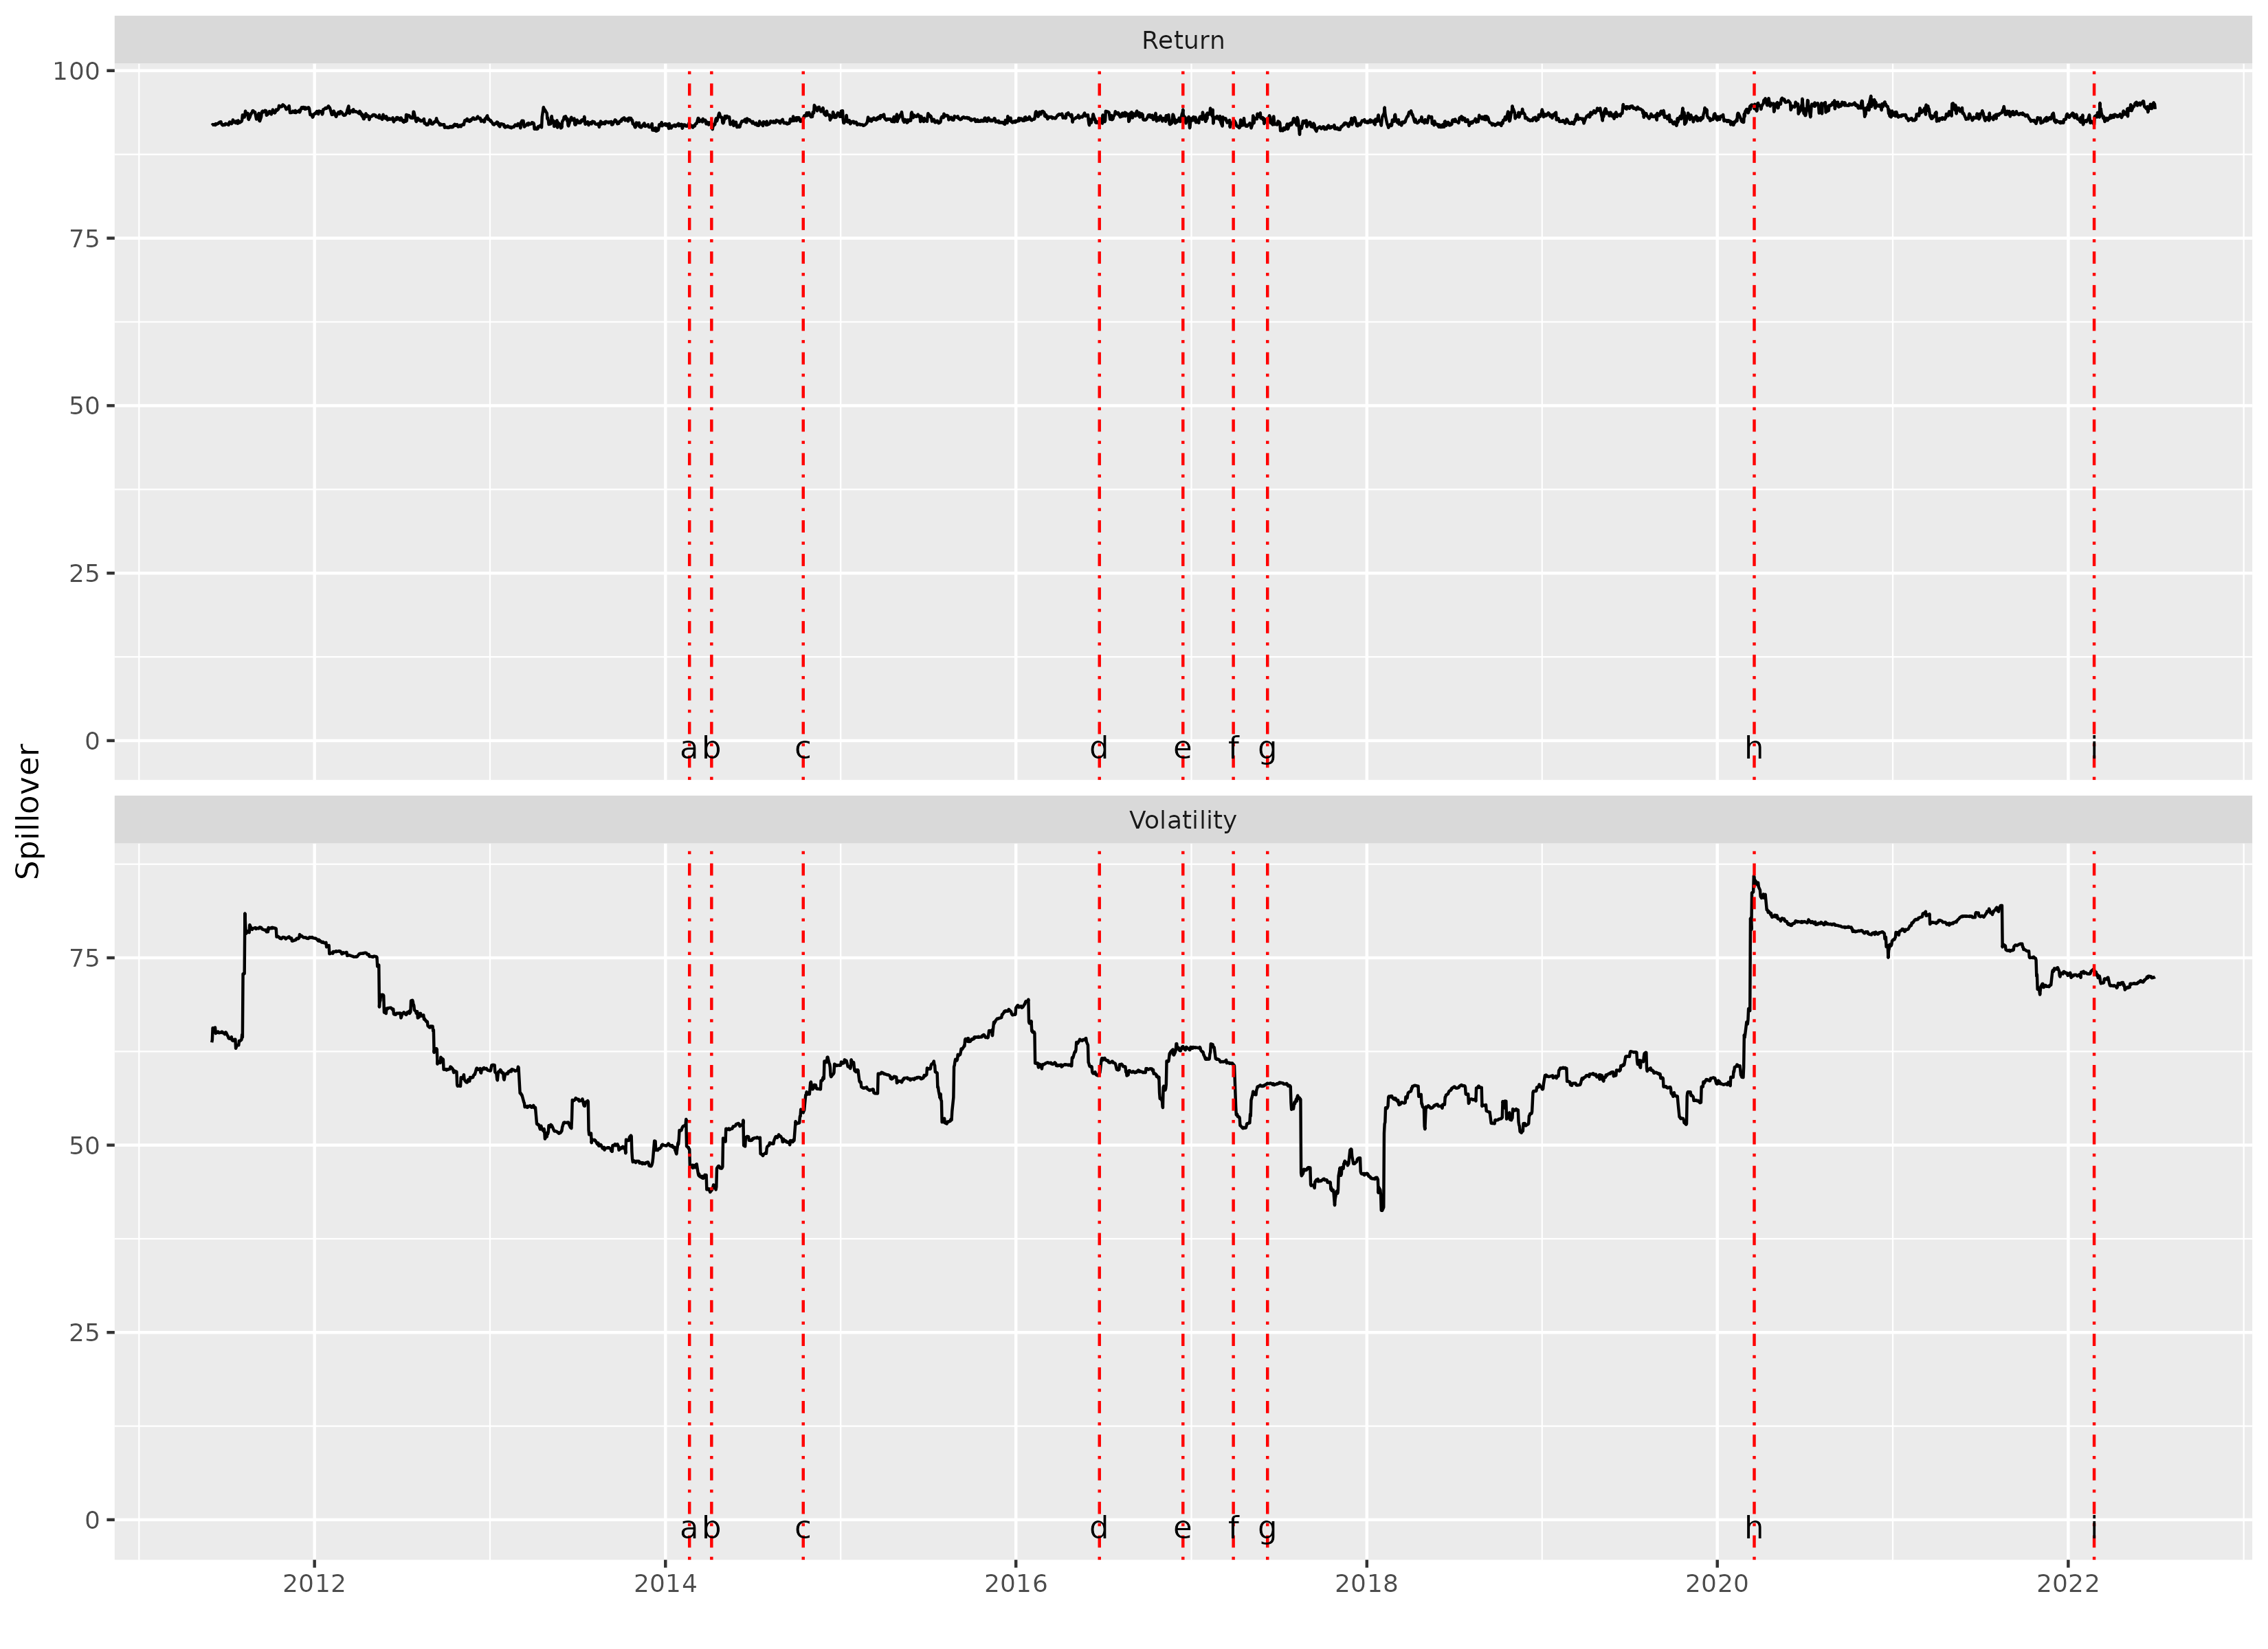
\includegraphics{plots/fig-TCI5.png}

}

\caption{\label{fig-TCI5}5th percentile}

\end{figure}

\begin{figure}[H]

{\centering 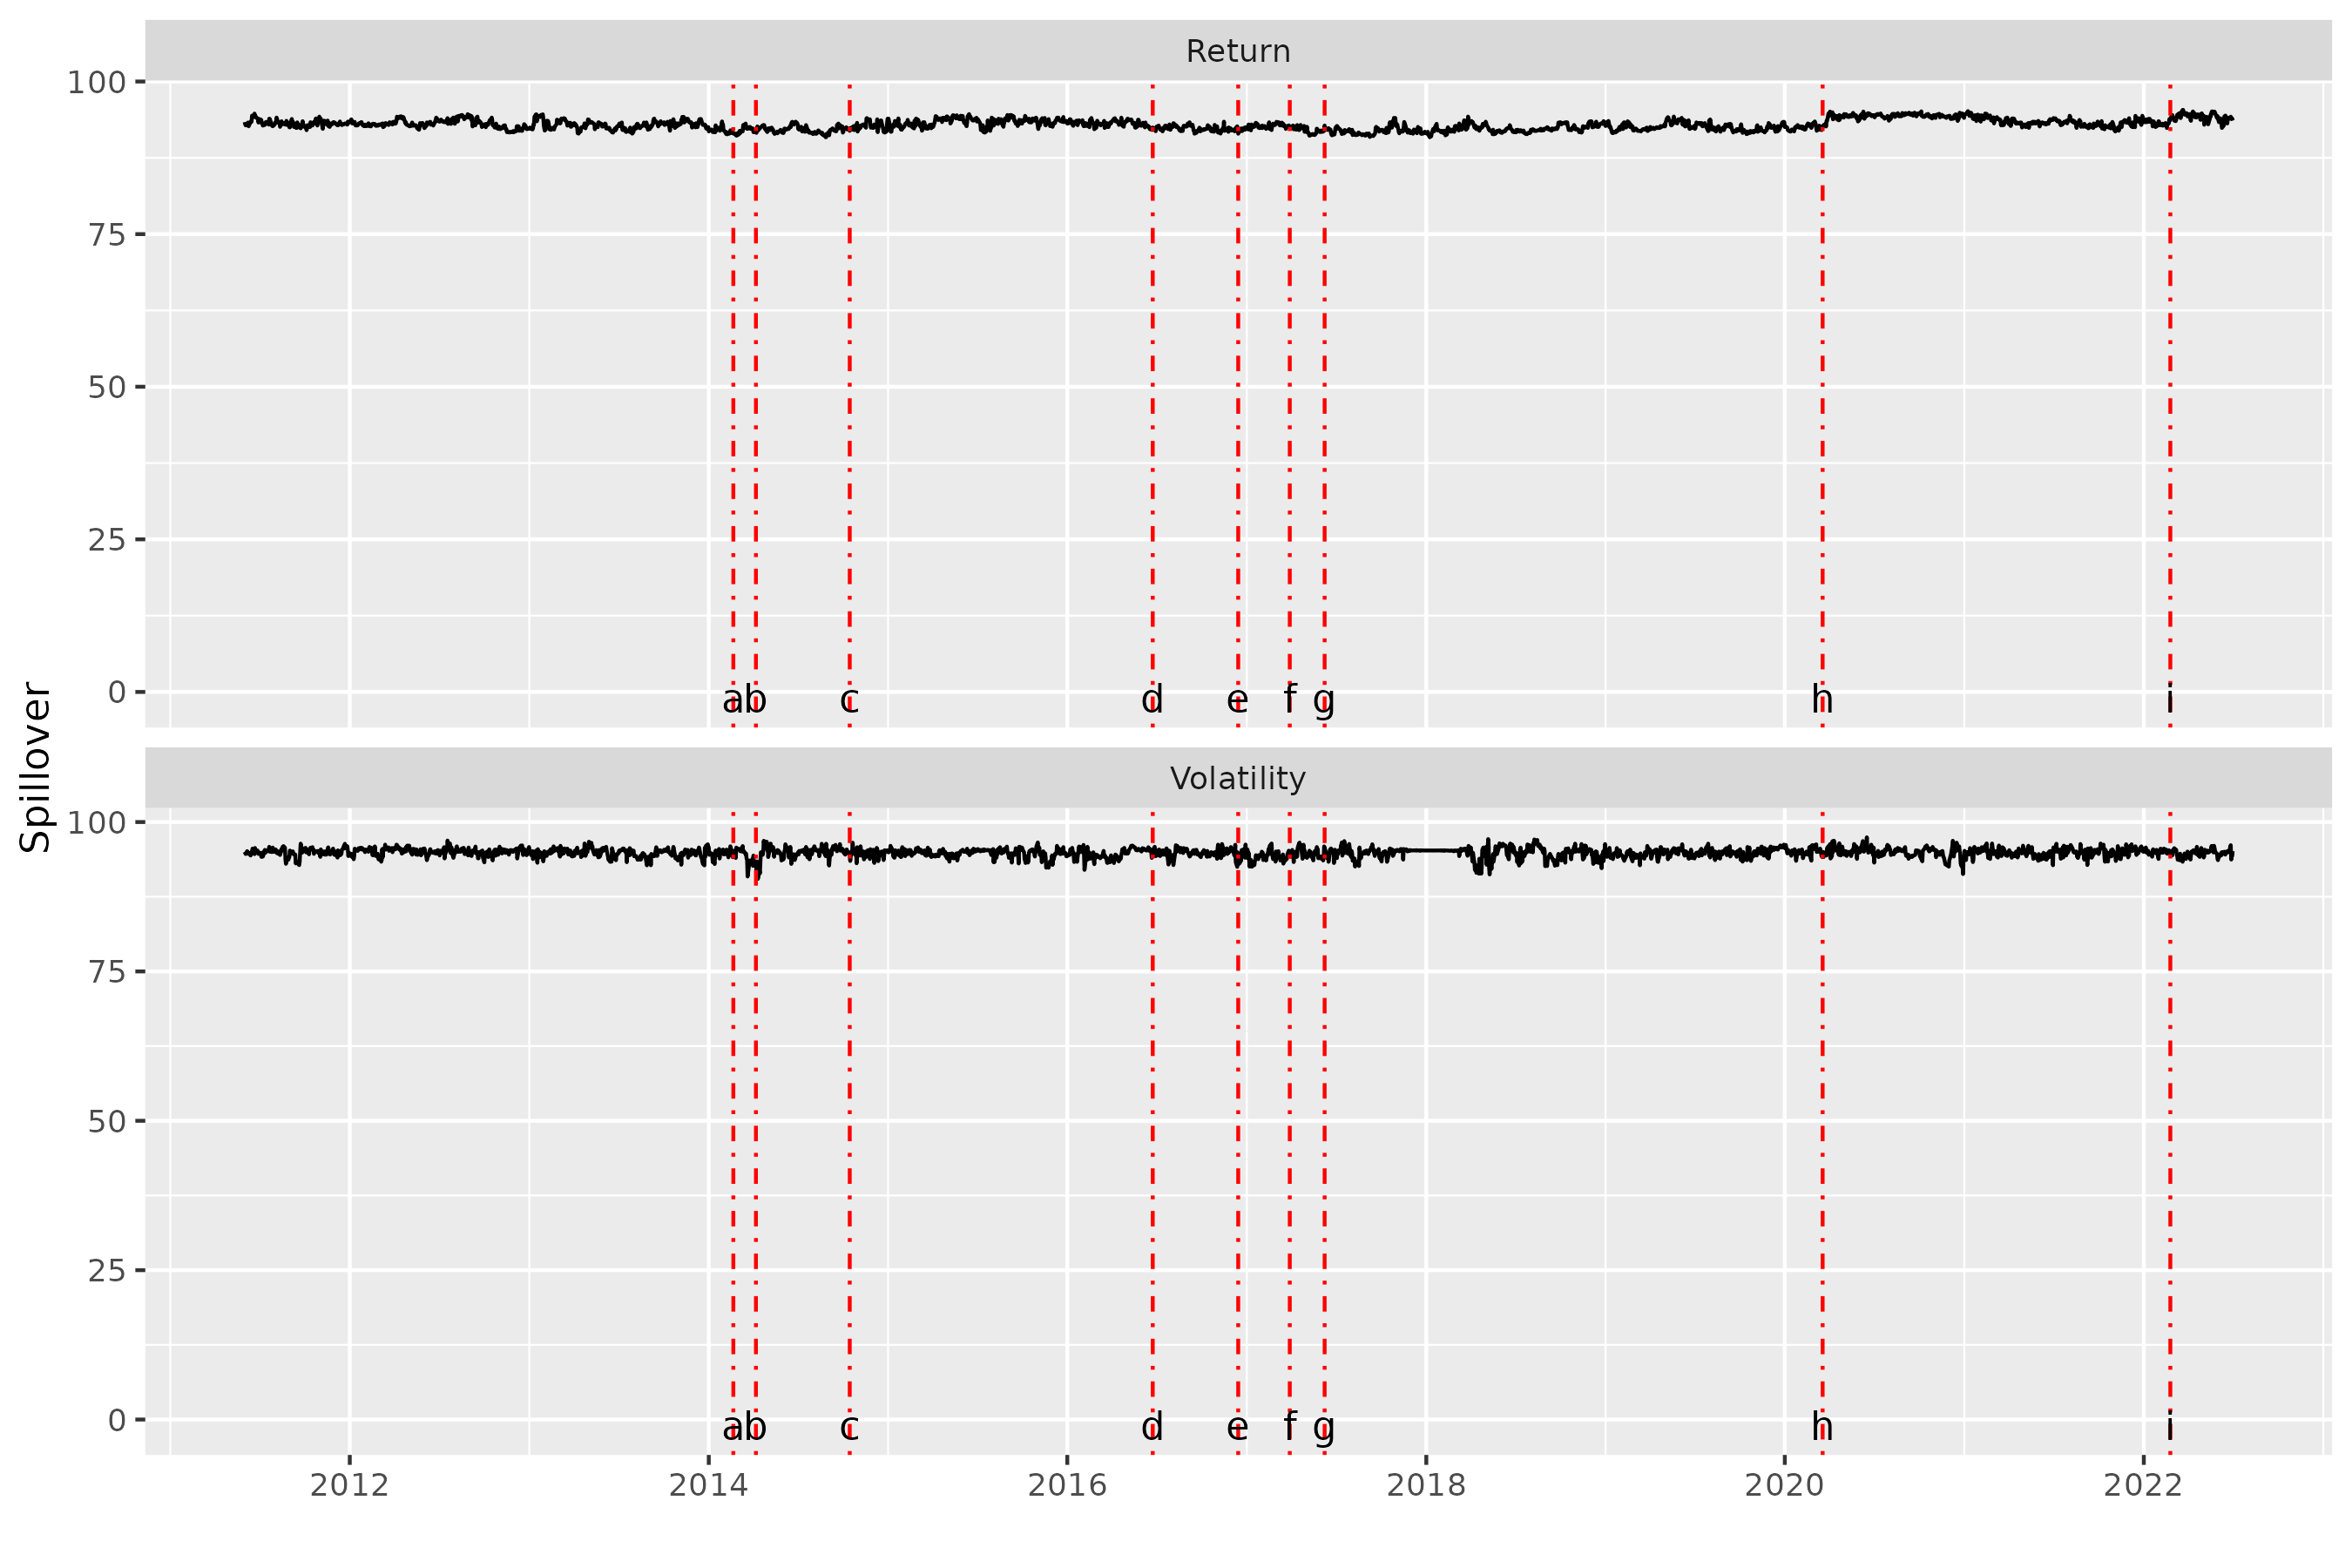
\includegraphics{plots/fig-TCI95.png}

}

\caption{\label{fig-TCI95}95\textasciitilde th\textasciitilde{}
percentile}

\end{figure}

\begin{figure}[H]

{\centering 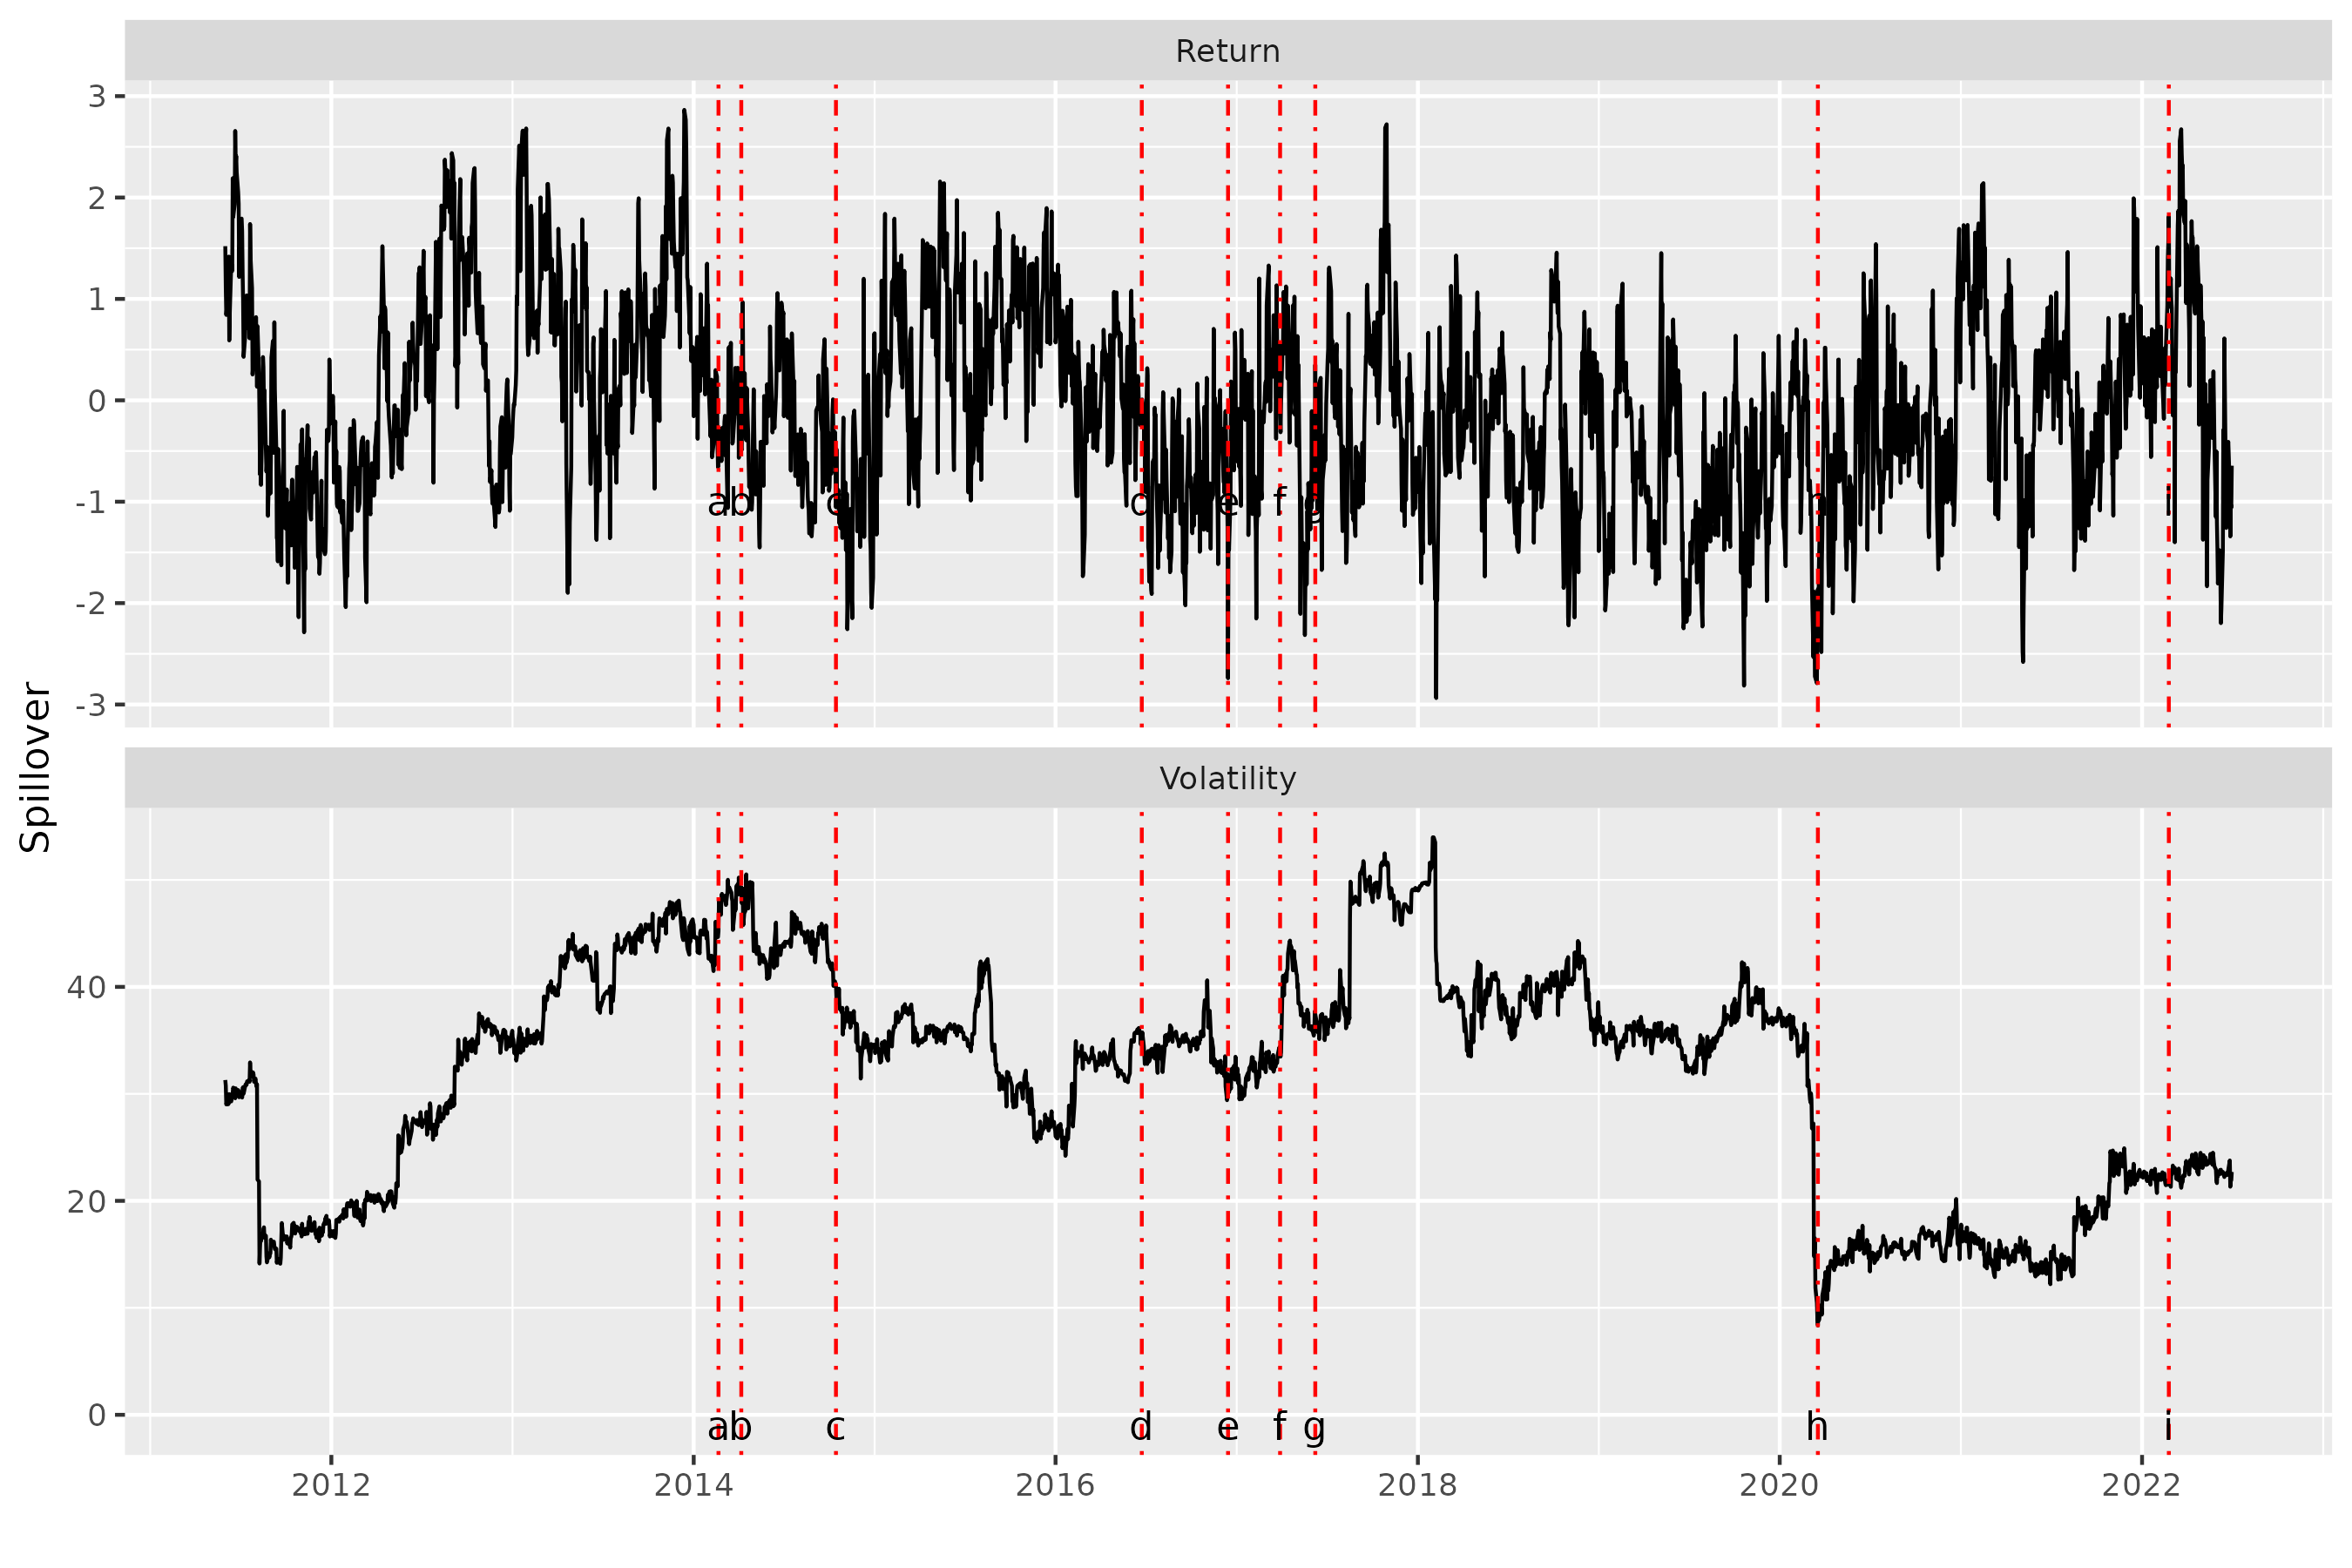
\includegraphics{plots/fig-TCIrtd.png}

}

\caption{\label{fig-TCIrtd}95th minus 5th percentile}

\end{figure}

Figure~\ref{fig-TCI50}, Figure~\ref{fig-TCI5}, Figure~\ref{fig-TCI95},
and Figure~\ref{fig-TCIrtd} comparing total connectedness of returns and
volatility. Vertical red dashed lines denote the dates of some important
events, which are described in Table~\ref{tbl-dates}.

\hypertarget{tbl-dates}{}
\begin{table}[H]
\caption{\label{tbl-dates}Important Dates }\tabularnewline

\centering
\begin{tabular}[t]{lll}
\toprule
label & date & description\\
\midrule
a & 2014-02-20 & Russia began annexation of Crimea\\
b & 2014-04-07 & Start of war in Donbas by pro-Russian activists\\
c & 2014-10-15 & October 2014 flash crash\\
d & 2016-06-23 & Brexit referendum\\
e & 2016-12-14 & Federal Reserve raises interest rates\\
\addlinespace
f & 2017-03-29 & the United Kingdom invokes article 50 of the Lisbon Treaty\\
g & 2017-06-08 & snap election held in the United Kingdom\\
h & 2020-03-18 & Dash for cash crisis in bond market peaks\\
i & 2022-02-24 & Russia initiated a special military operation in Donbas\\
\bottomrule
\end{tabular}
\end{table}

The TOTAL connectedness index at the conditional median (a measure of
the average connectedness) and extremes for returns and volatility
systems are presented in Figure 11. In the spirit of Ando,
Greenwood-Nimmo, and Shin (2022), the final pair of Figures illustrate
the relative tail dependence (RTD) calculated as the difference between
the 95th and 5th percentile. Positive (negative) values of RTD indicate
stronger (weaker) dependence in the right tail compared to the left
tail. For returns, we interpret increases (decreases) in RTD as evidence
of a rising (falling) connectedness of financial performance of defense
stocks. For volatility, we interpret increases (decreases) in RTD as
evidence of rising (falling) connectedness of financial uncertainty in
defense stocks, or more succinctly, rising (failing) financial fragility
as positive (negative) volatility shocks disseminate through the system
of defense stocks

Figure~\ref{fig-TCI50} illustrates that in normal conditions the
connectedness in the returns system tends to be larger than that of the
volatility system of defense stocks. The connectedness reaches its peak
at point h (the `dash for cash' event) at the beginning of the COVID-19
pandemic. Importantly, while the connectedness levels are greater in the
returns system the volatility system connectedness exhibits higher
sensitivity to shocks, with the largest regime shift at point h.

Figure~\ref{fig-TCI5} and Figure~\ref{fig-TCI95} illustrate the time
variation of total system connectivity at the 5th and 95th percentiles
of the conditional distributions. It is noted that return system
connectedness is persistently high (above 90) at both tails of the
conditional distribution, while volatility system connectedness in
period of extremely low volatility (5th percentile) is more sensitivity
temporal events. The top panel in Figure~\ref{fig-TCIrtd} illustrates
that time variation of the RTD for returns is symmetrical over the
period, indicative of equally spread of positive and negative feedback
loops in return spillover effects. In contrast, the bottom panel in
Figure~\ref{fig-TCIrtd} shows the persistent one-sidedness of the RTD
for the volatility series, with the right tail of the condition
distribution dominant throughout the period. This asymmetry suggests
that volatility spillovers across defense is amplified by the size of
that uncertainty. Taken together, these results suggest that only the
total connectedness of defense stocks' volatility is affected by the
size of the volatility in the system.

Finally, we consider the chronological order of prominent global
economic and conflict turmoil events in the context of median and
extreme linkages in the systems of volatility and returns. Some striking
patterns emerge in this chronological ordering. Firstly, from the
beginning of the conflict in Crimea (a + b) to the Brexit referendum (d)
the RTD for volatility trends down, indicative of an increase in
resilience (reduction in fragility) in the defense system. This is
coupled with the fact that RTD is mostly positive for the return system
in this sub-period. Taken together, these findings suggest that upper
tail returns (right tail of the conditional distribution) in this period
create some spillover effects, while the financial fragility of the
system weakens. There is also a notable regime shift at dash for cash
date (h) where the financial fragility (the volatility system) fell by
50\% (TCI = 40 to TCI = 20).

\hypertarget{individual-connectivity}{%
\subsubsection{Individual connectivity}\label{individual-connectivity}}

\begin{figure}[H]

{\centering 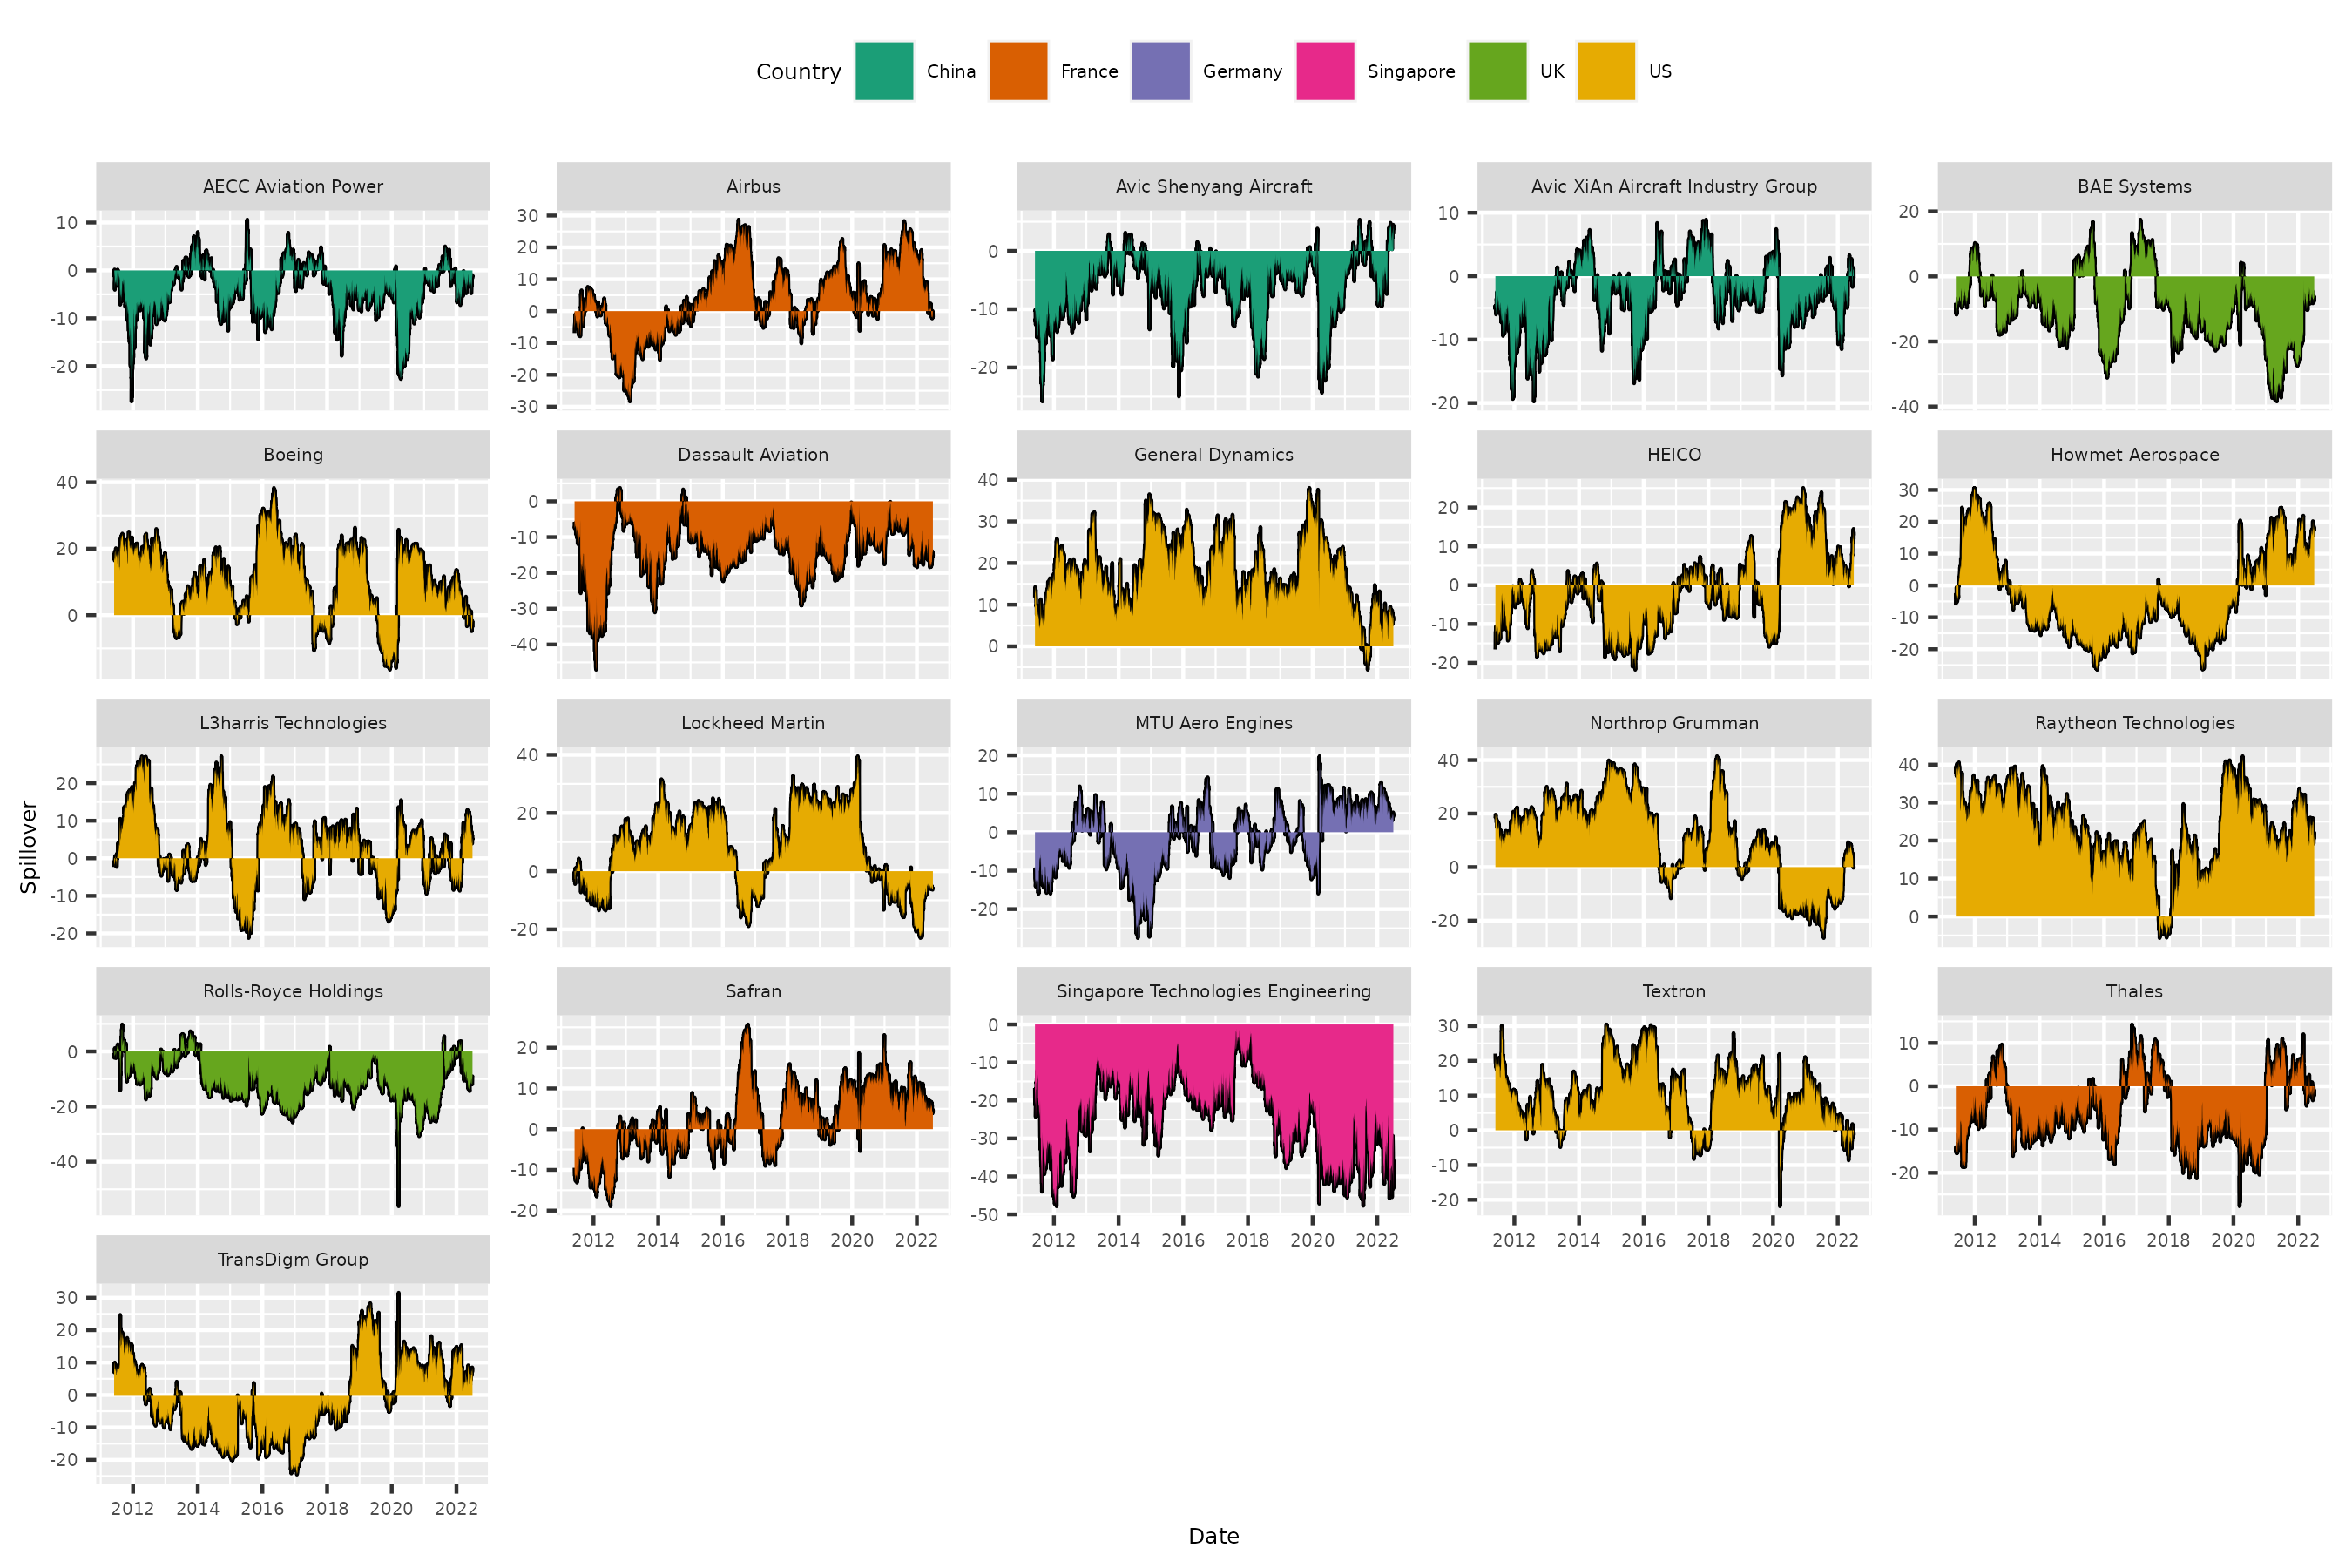
\includegraphics[width=1\textwidth,height=\textheight]{plots/fig-rtnnet50.png}

}

\caption{\label{fig-rtnet50}Net spillover effects for the stock returns
at the median}

\end{figure}

\begin{figure}[H]

{\centering 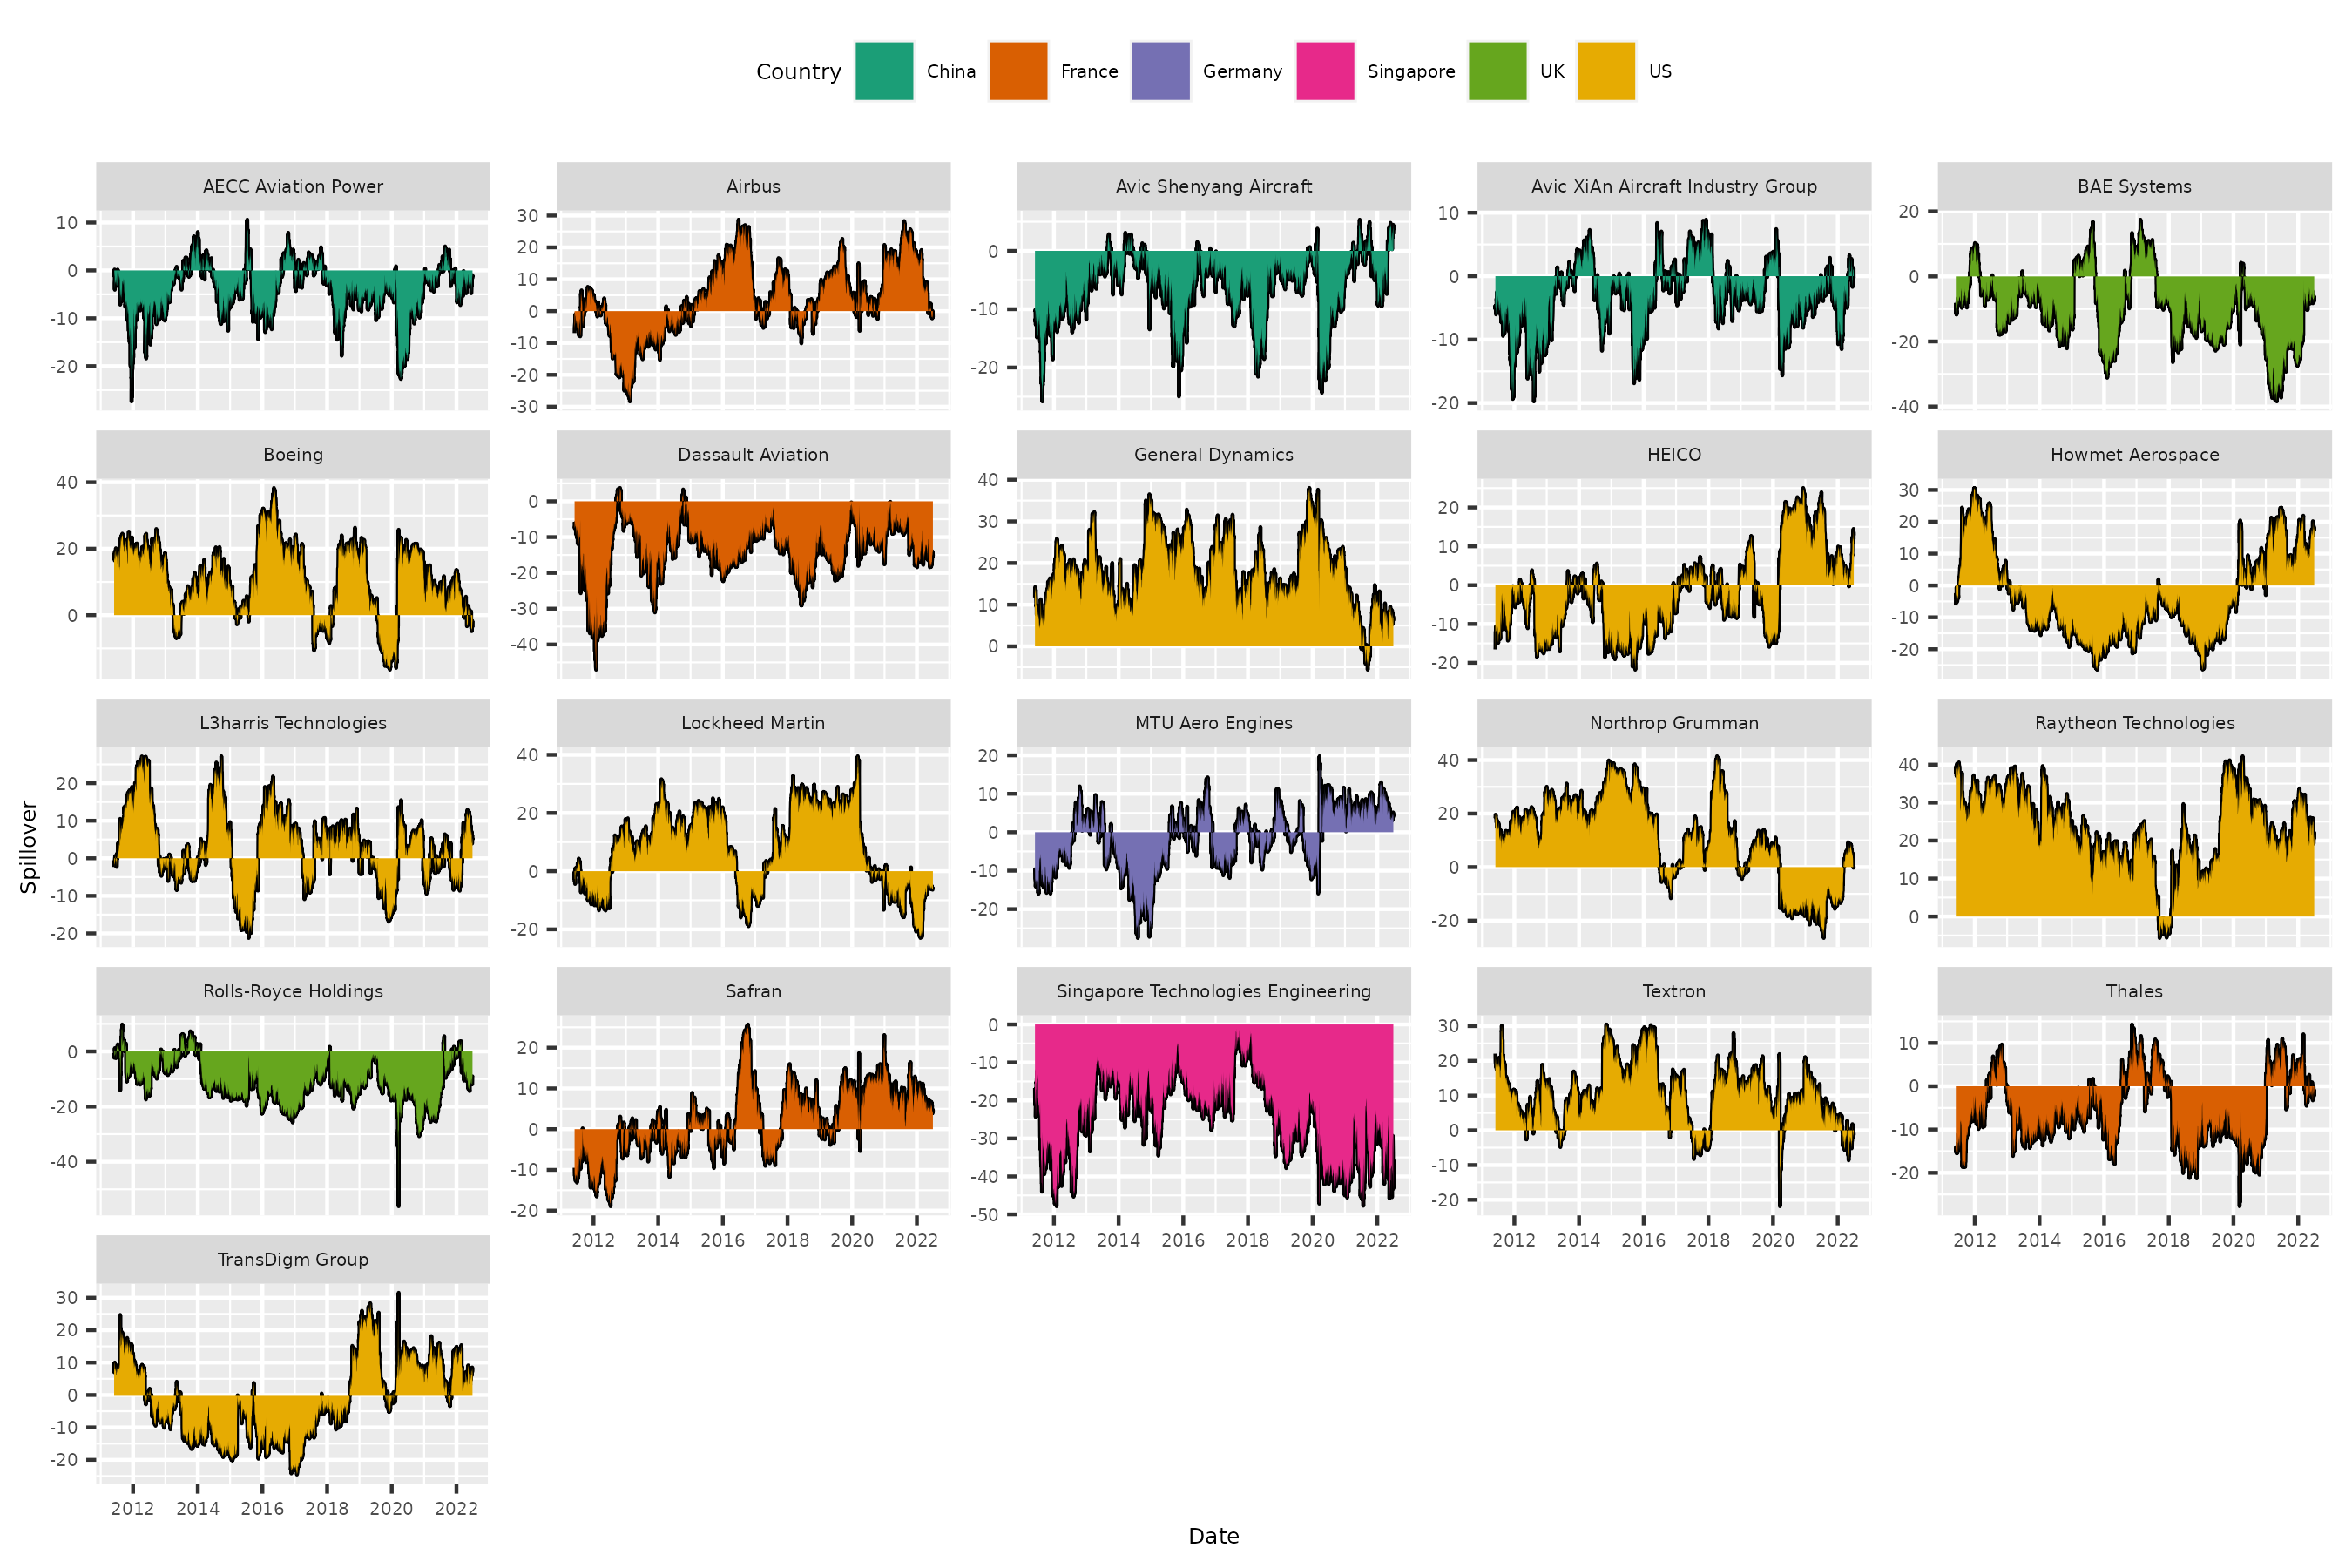
\includegraphics{plots/fig-rtnnet5.png}

}

\caption{\label{fig-rtnet5}Net spillover effects for stock returns at
the 5th percentile}

\end{figure}

\begin{figure}[H]

{\centering 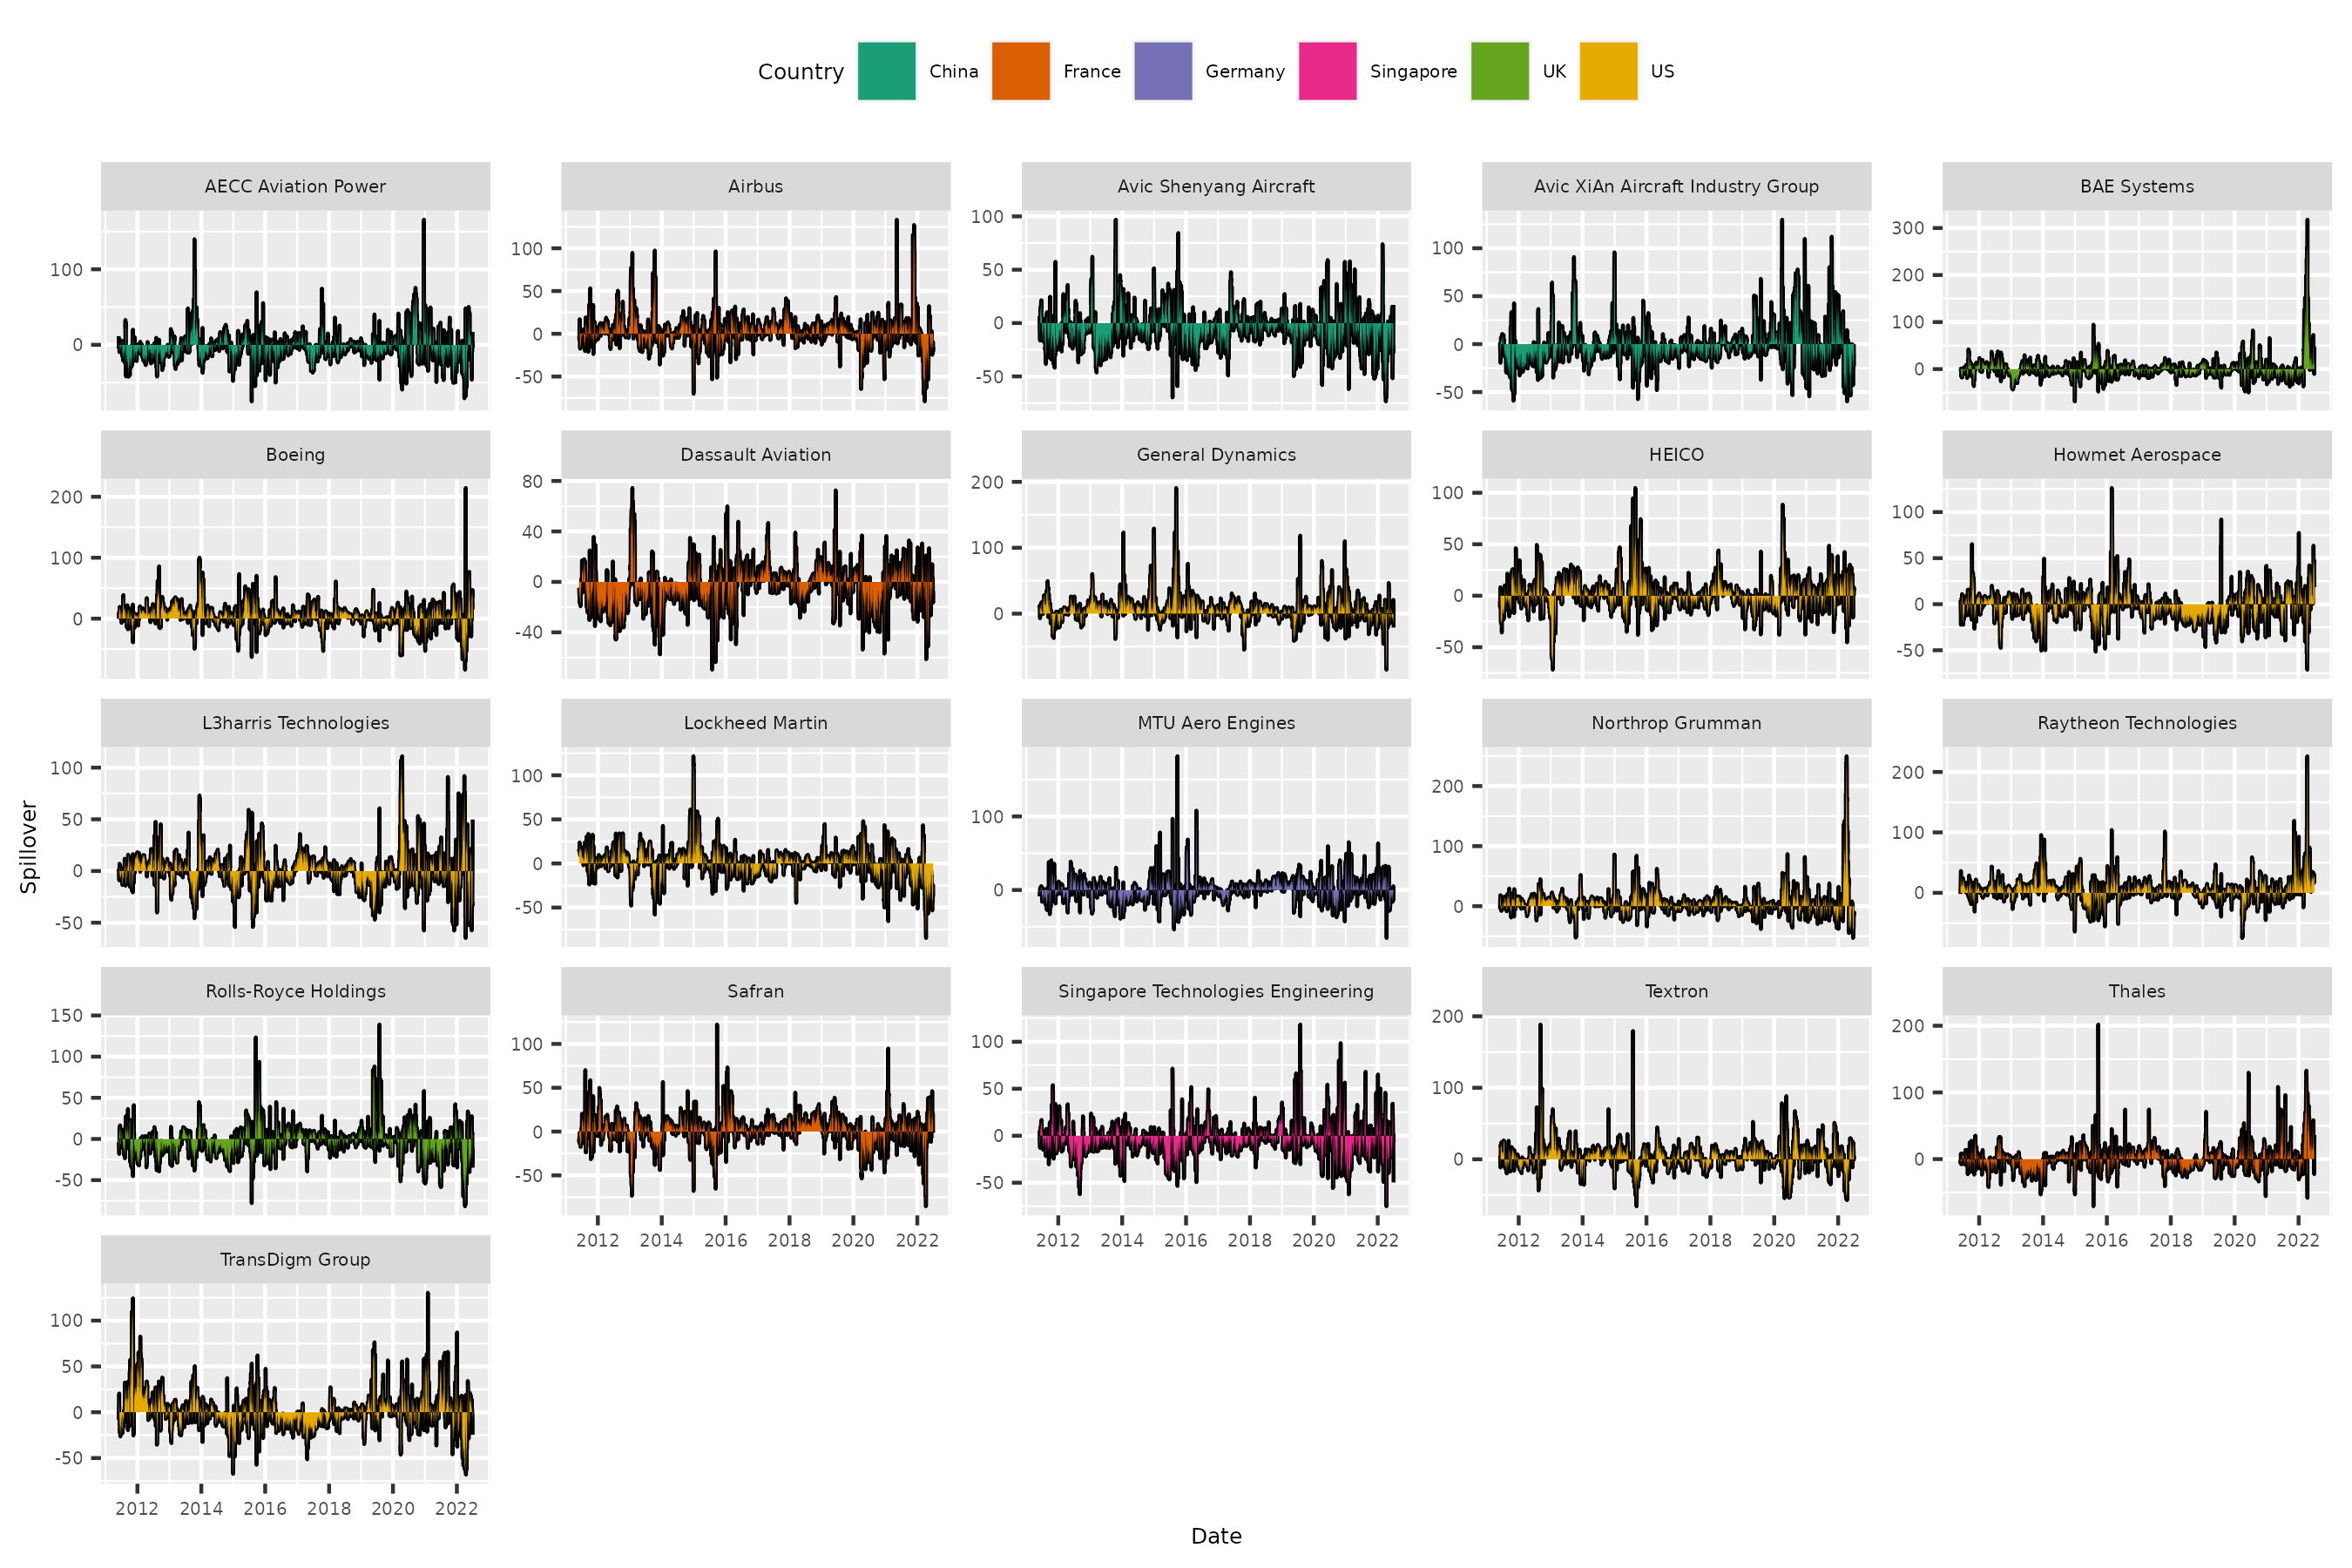
\includegraphics{plots/fig-rtnnet95.png}

}

\caption{\label{fig-rtnet95}Net spillover effects for stock returns at
the 95th percentile}

\end{figure}

\begin{figure}[H]

{\centering 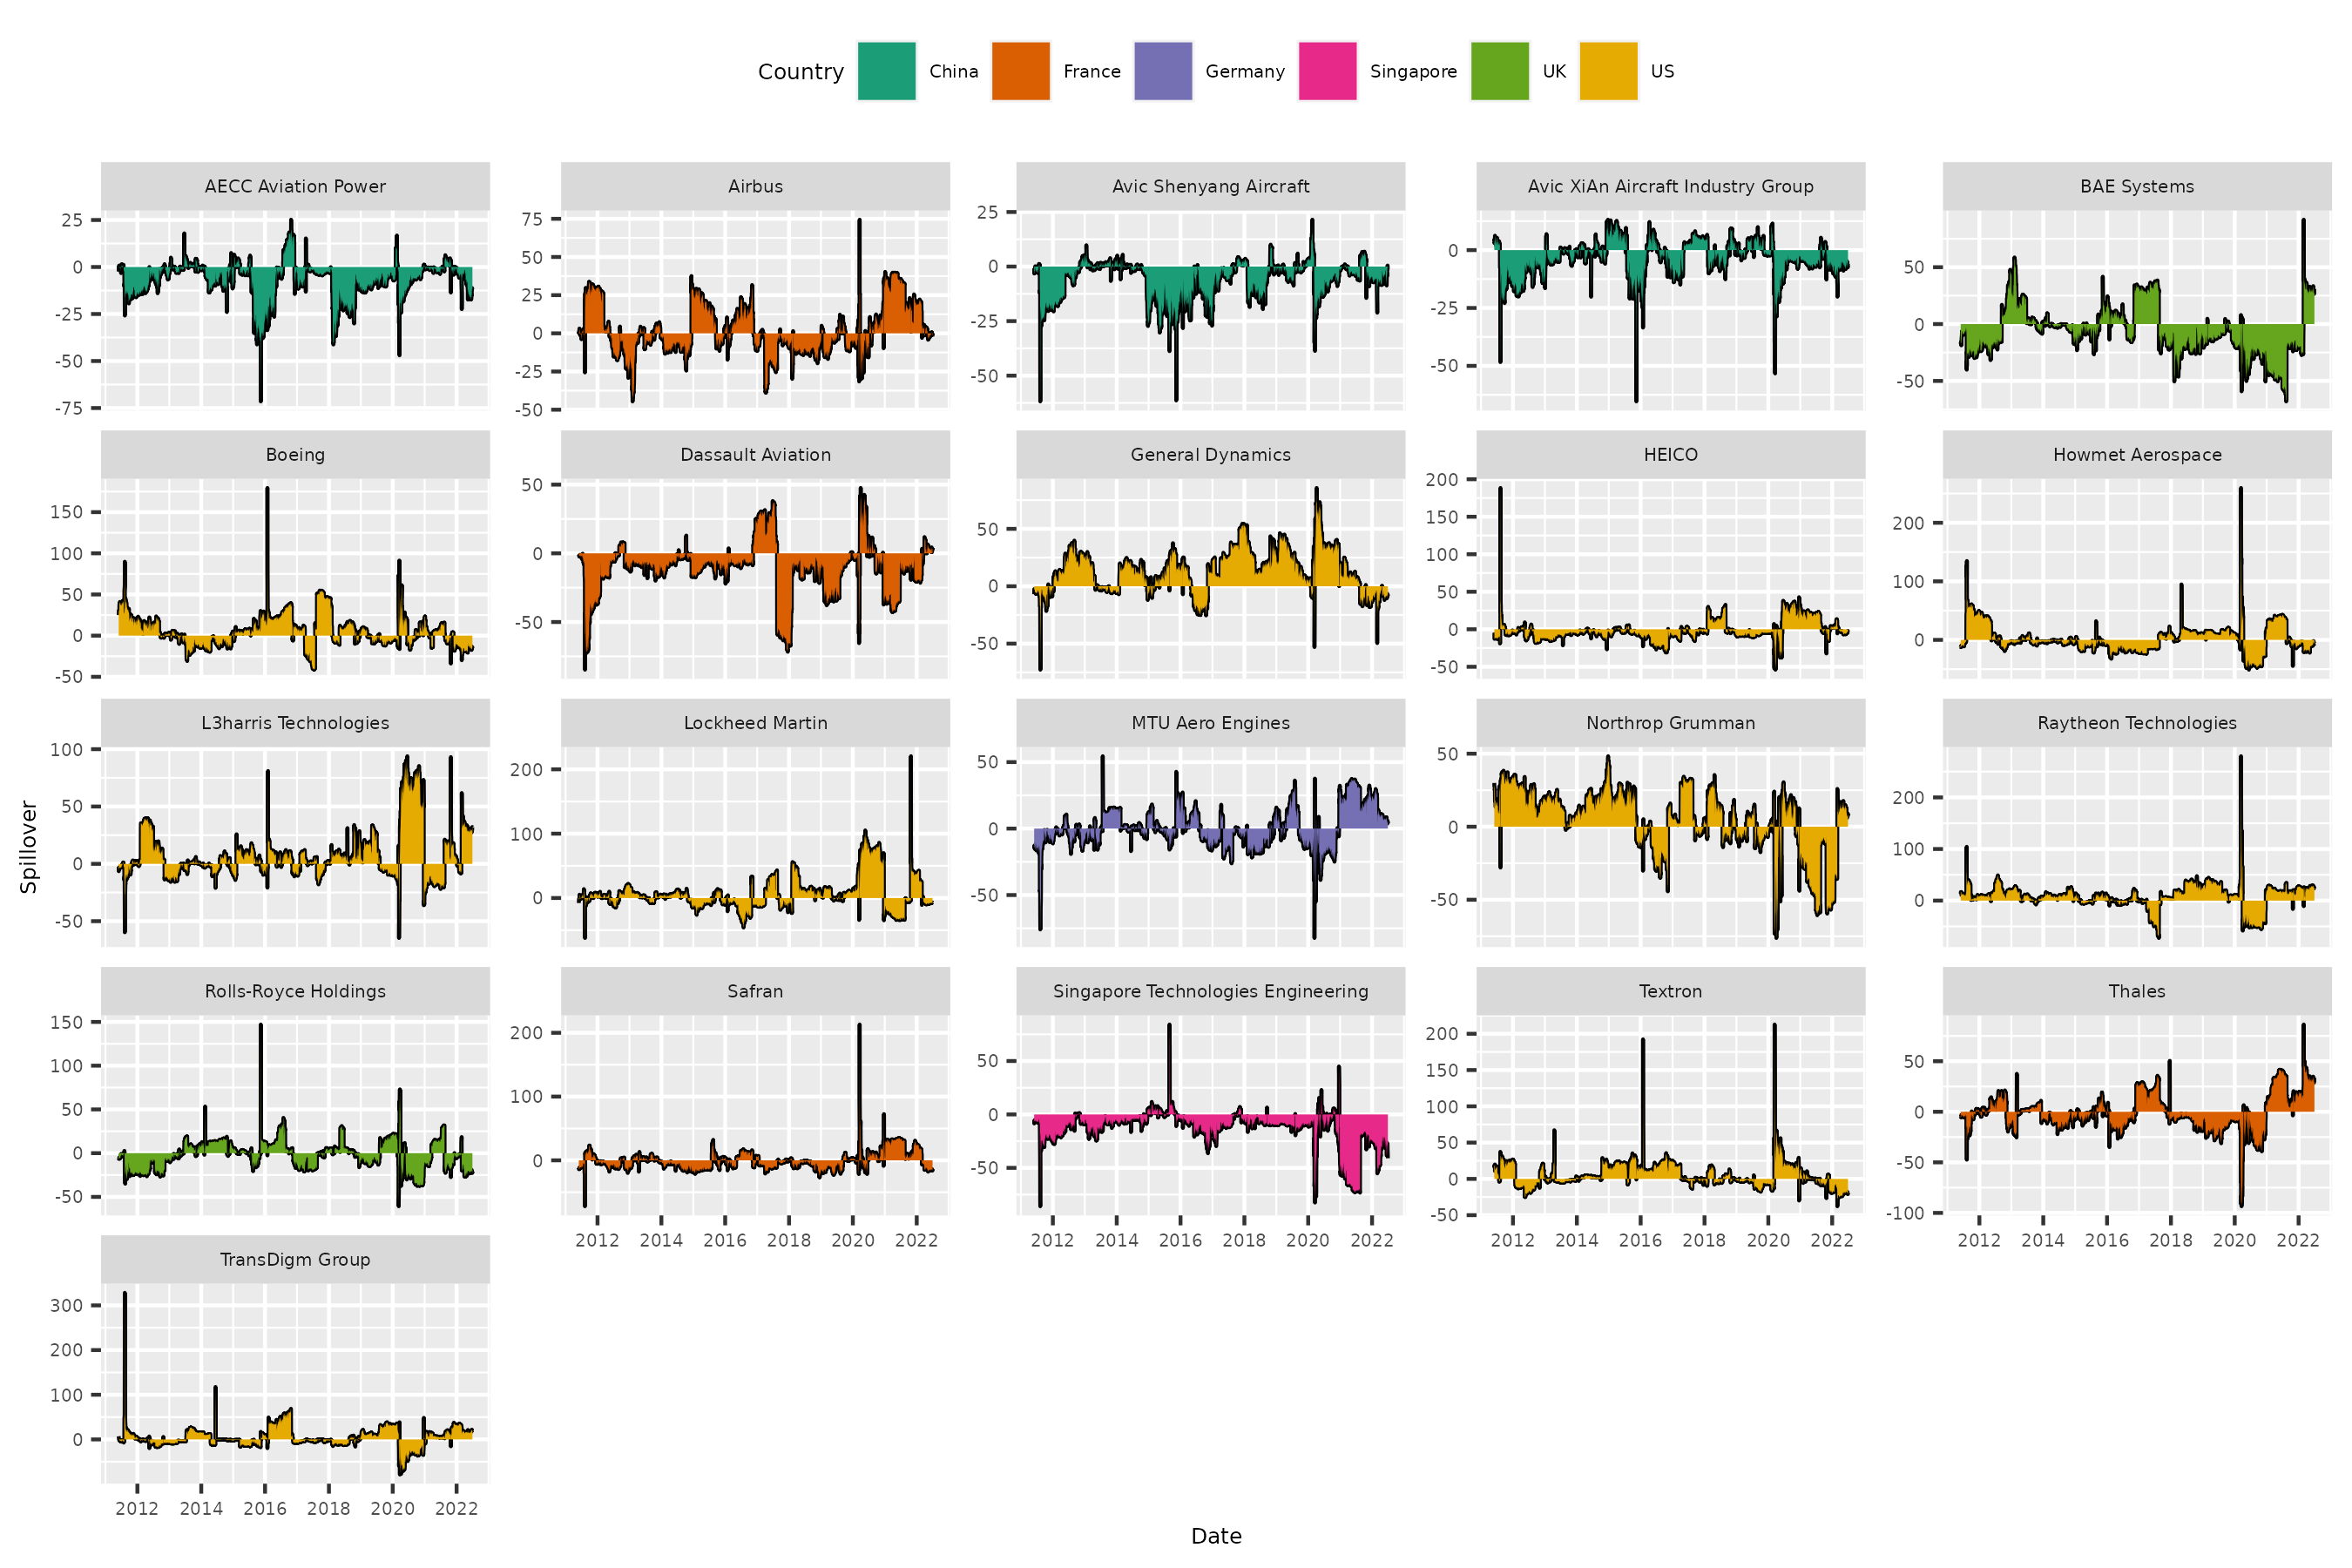
\includegraphics{plots/fig-volnet50.png}

}

\caption{\label{fig-volnet50}Net spillover effects for stock
volatilities at the median}

\end{figure}

\begin{figure}[H]

{\centering 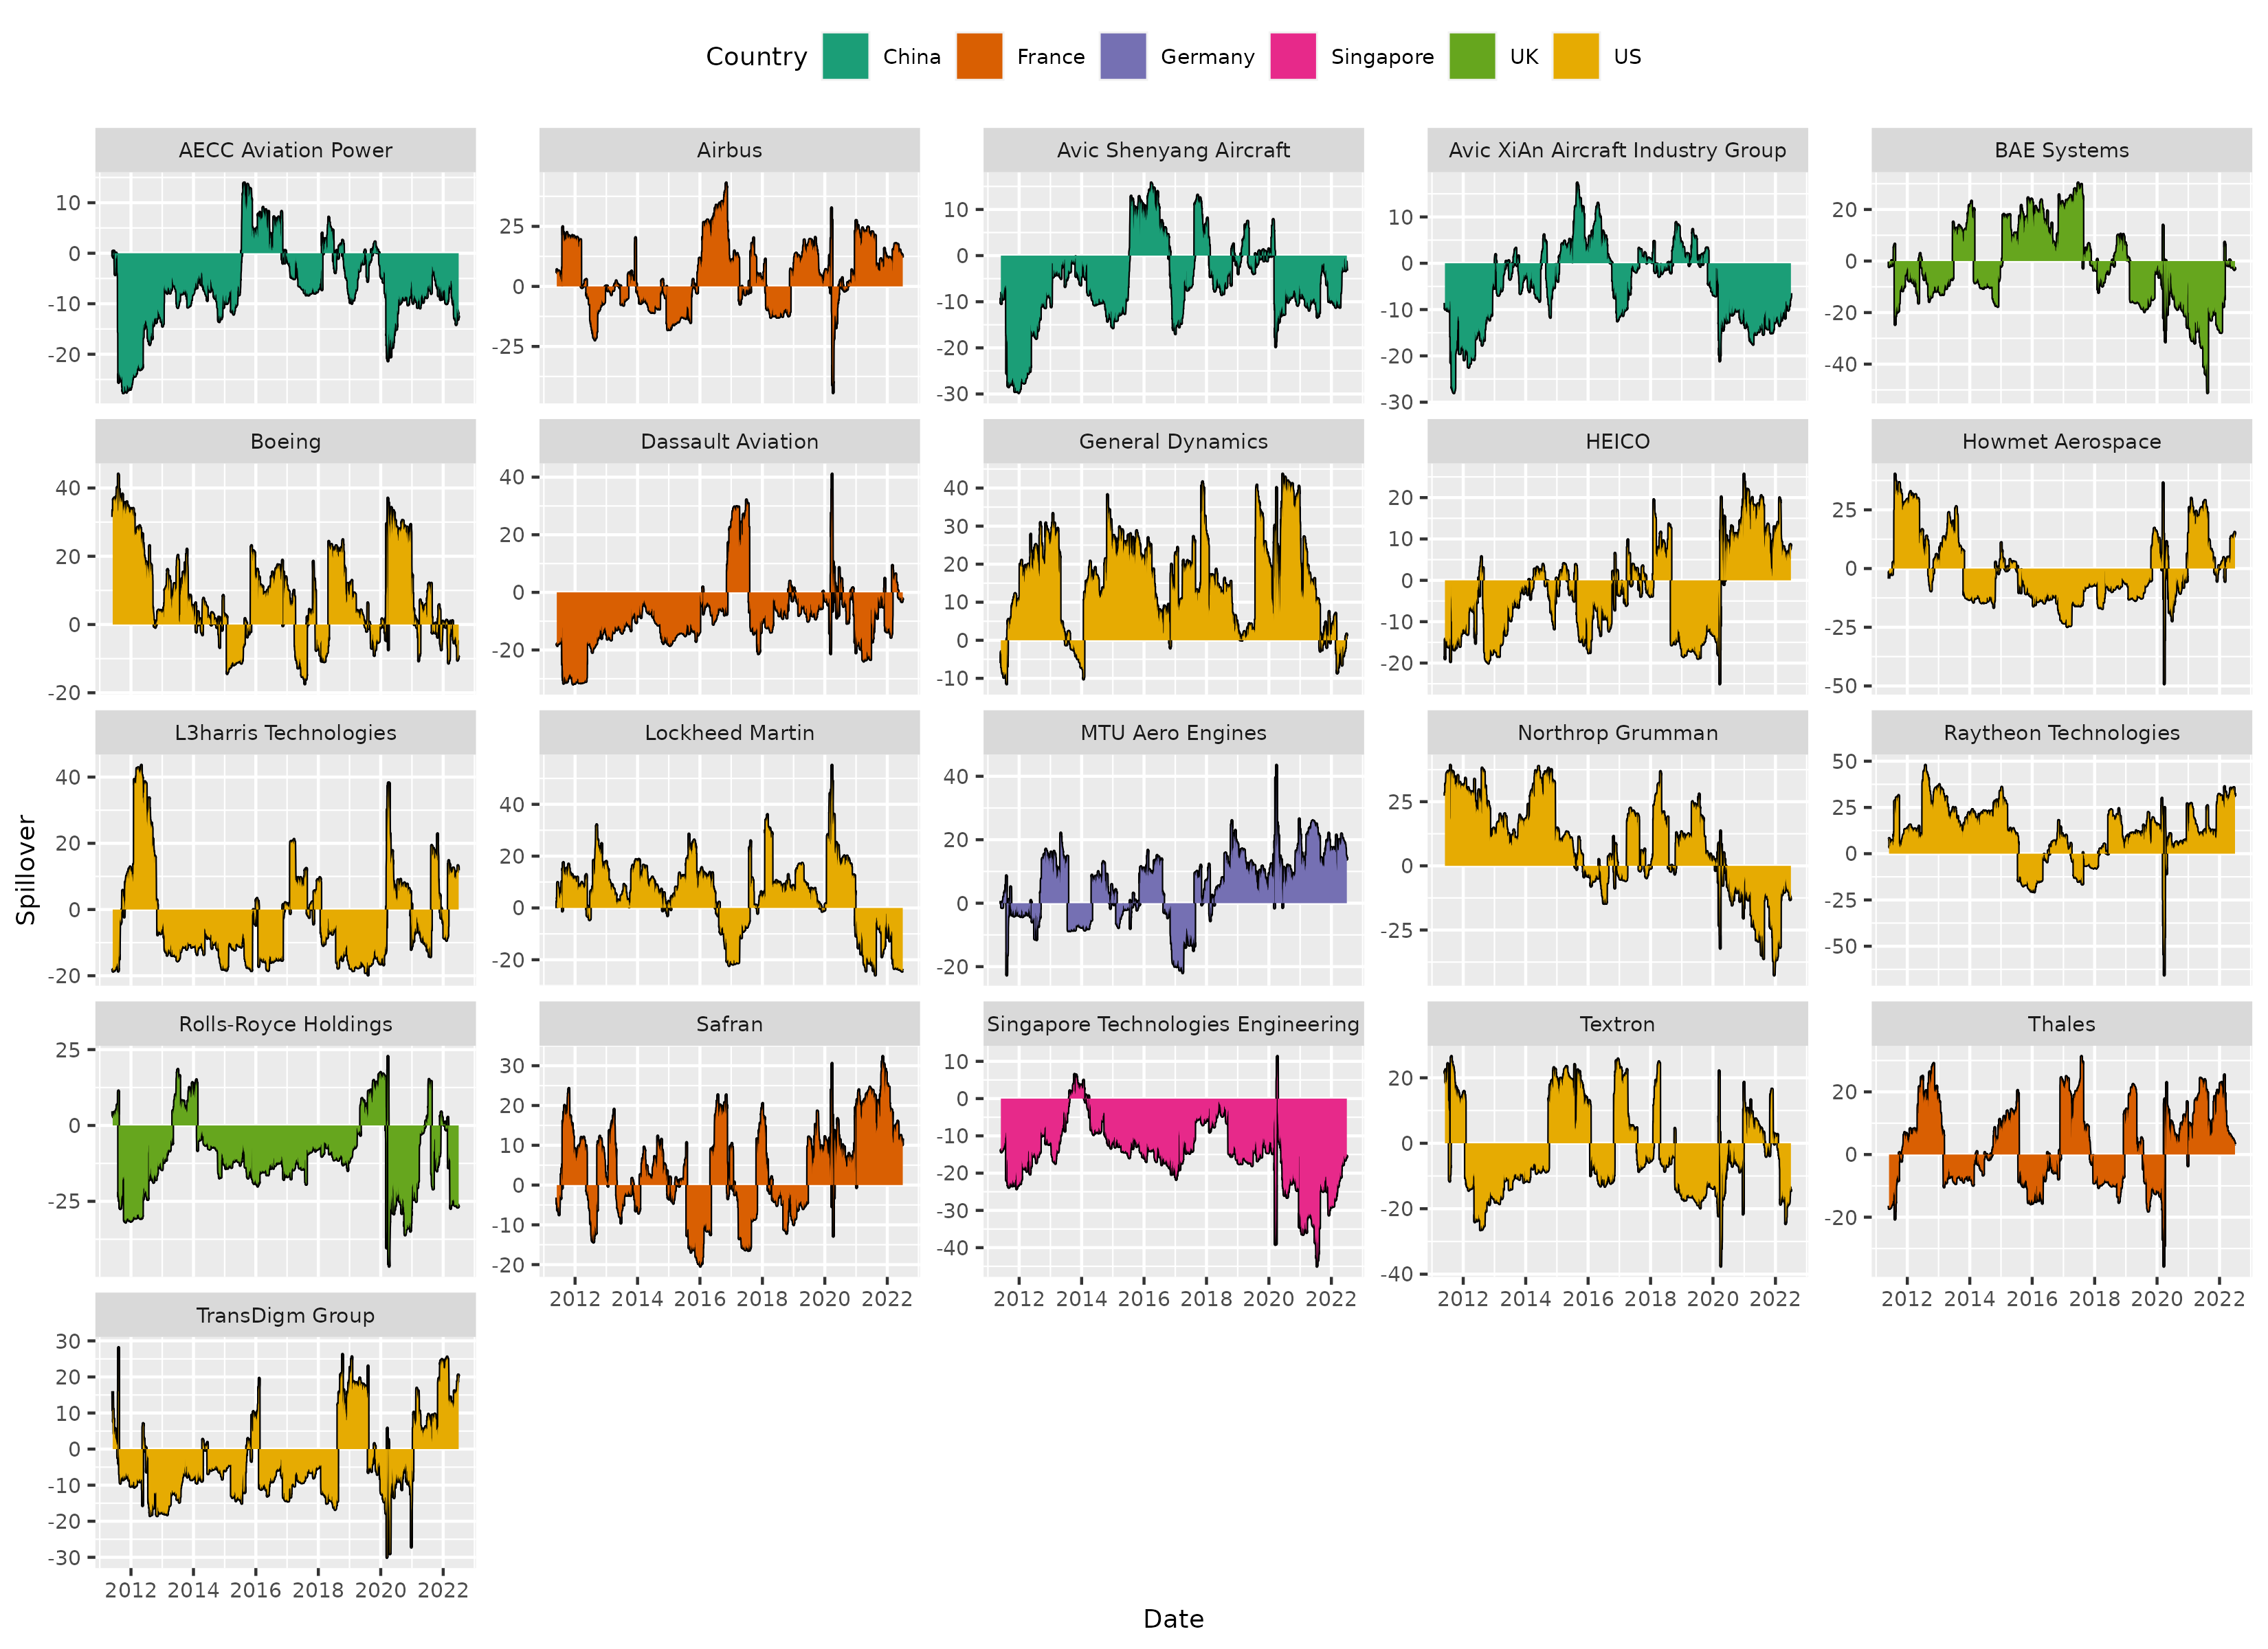
\includegraphics{plots/fig-volnet5.png}

}

\caption{\label{fig-volnet5}Net spillover effects for stock volatilities
at the 5th percentile}

\end{figure}

\begin{figure}[H]

{\centering 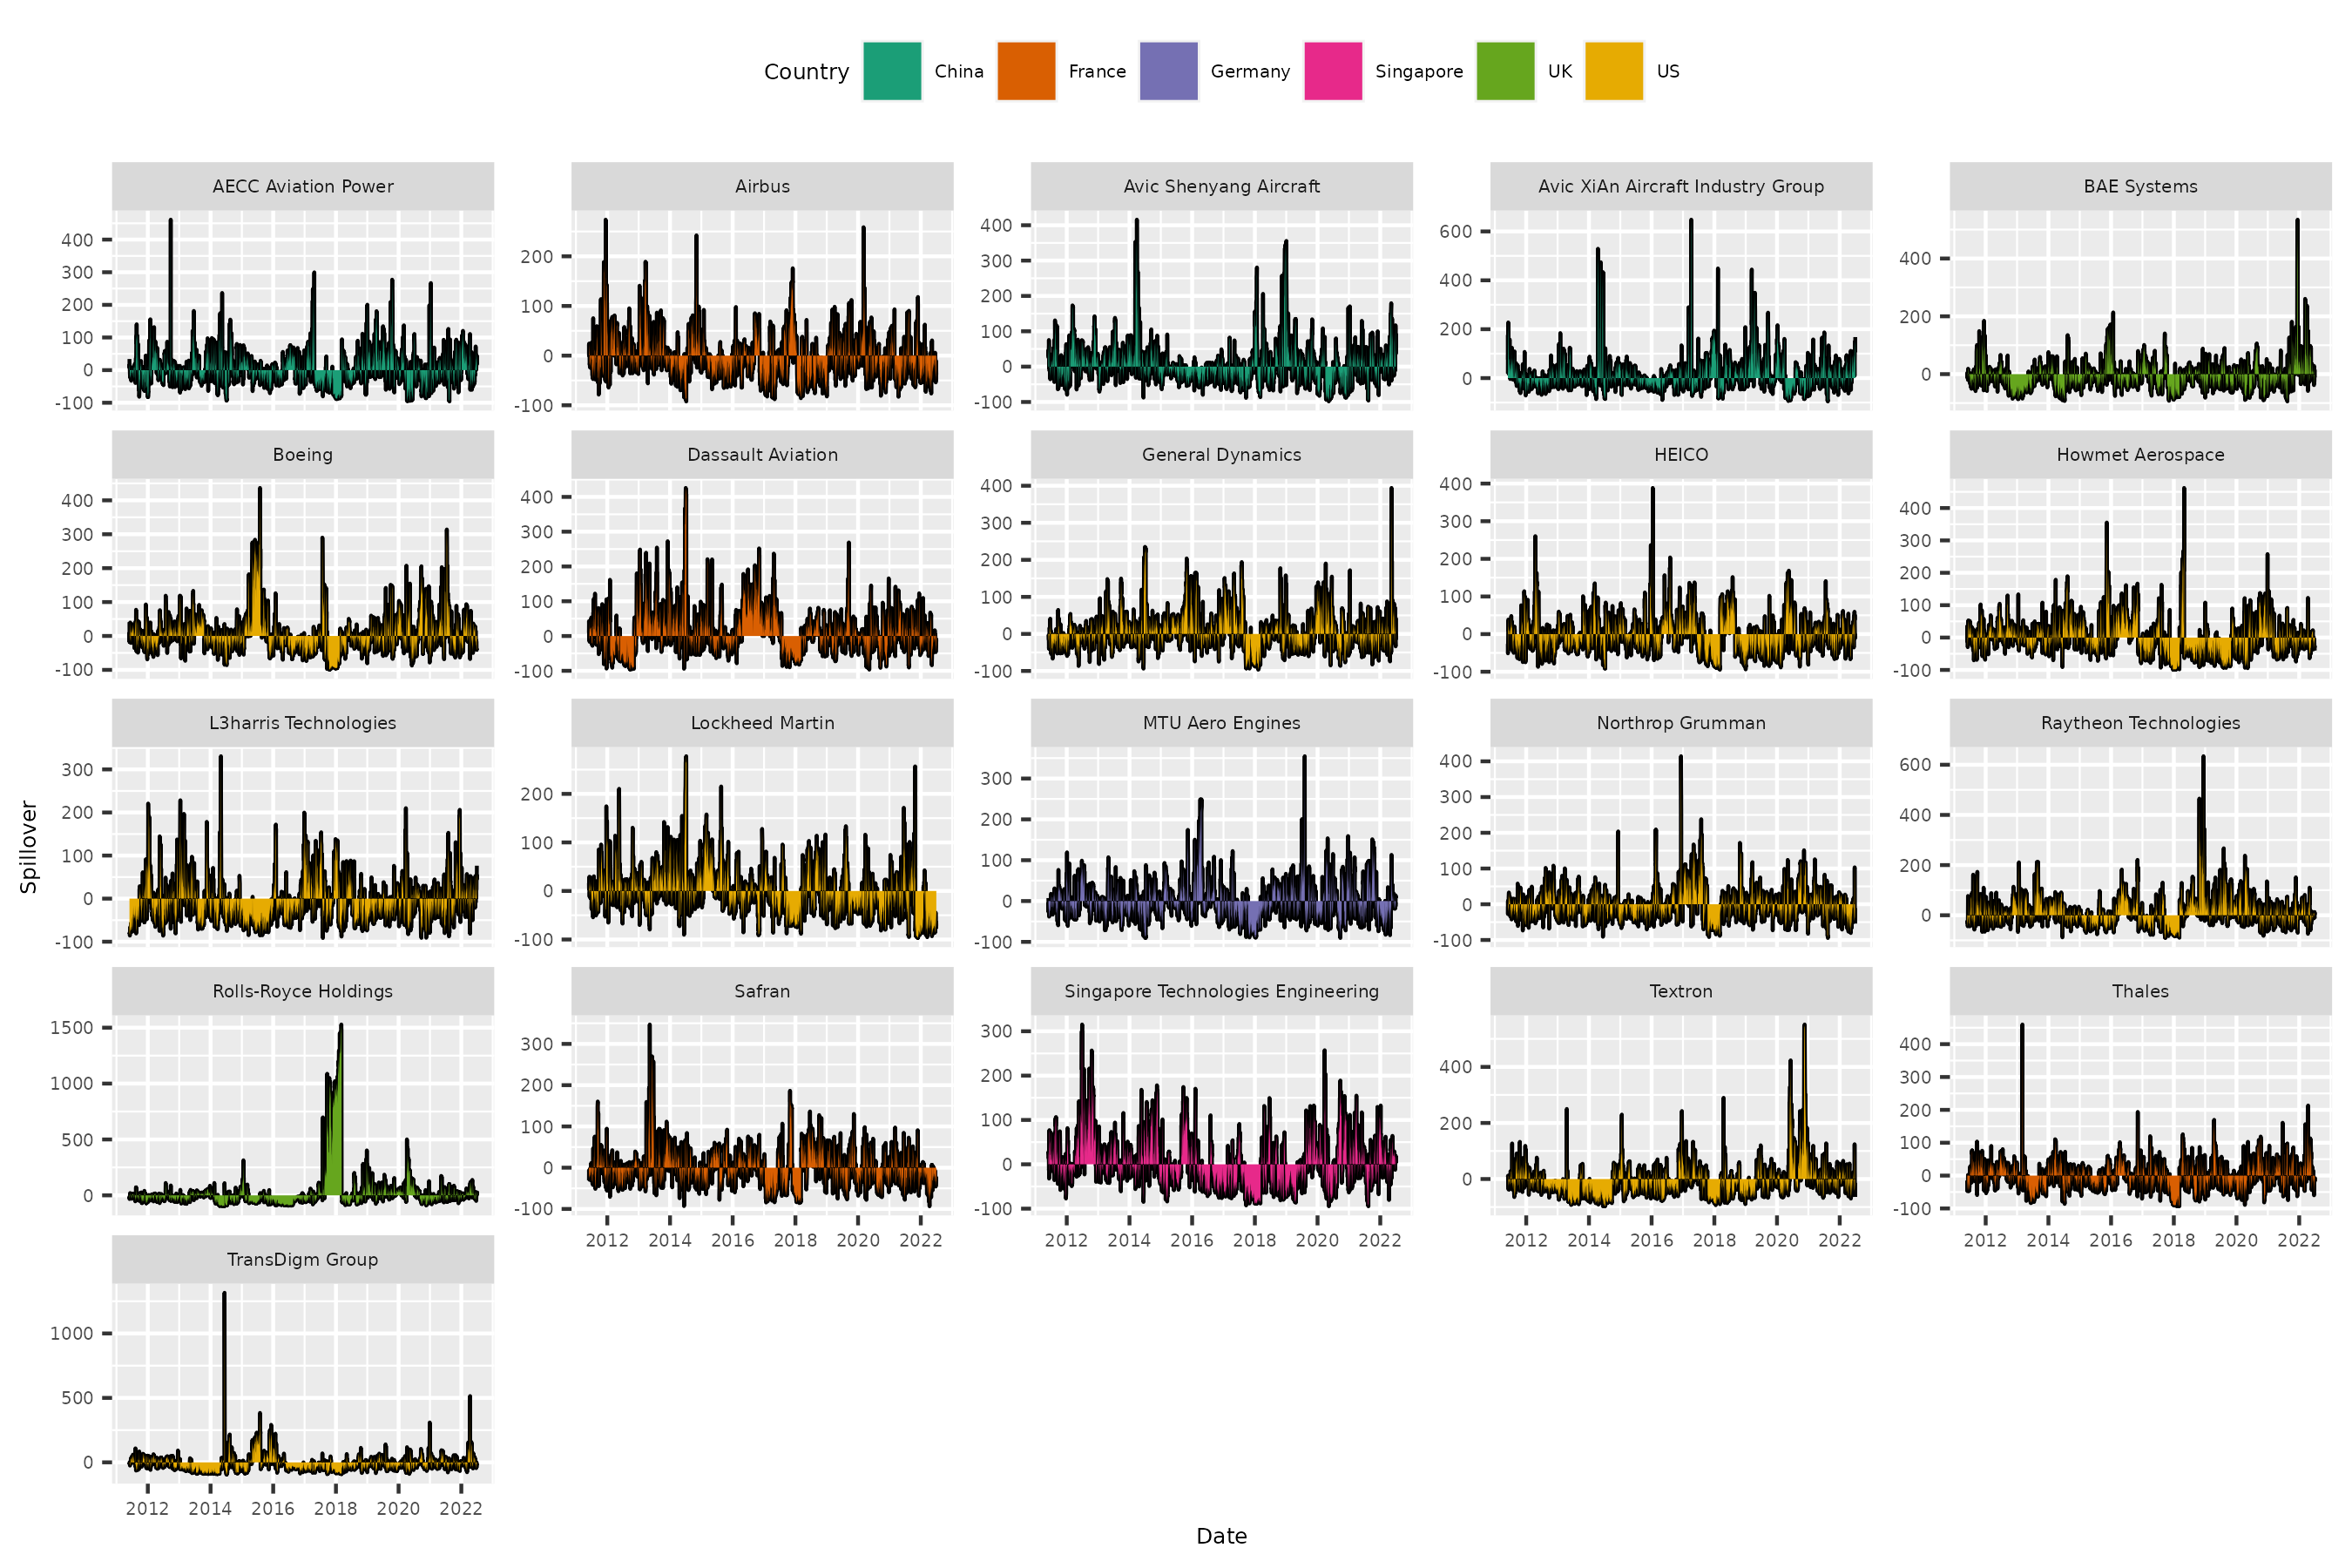
\includegraphics{plots/fig-volnet95.png}

}

\caption{\label{fig-volnet95}Net spillover effects for stock
volatilities at the 95th percentile}

\end{figure}

To disentangle the total connectedness variation further explore the net
spillover effects
\(T_{\cdot \leftarrow i,(\tau)}^h -F_{i \leftarrow \cdot,(\tau)}^h\).
Figure~\ref{fig-rtnet50} , Figure~\ref{fig-rtnet5} and,
Figure~\ref{fig-rtnet95} present the Net spillover of individual stock
returns at the median, lower and upper quantiles respectively.
Figure~\ref{fig-volnet50} , Figure~\ref{fig-volnet5} and,
Figure~\ref{fig-volnet95} present the same estimates for stock
volatilities.

We group these plots by country and some interesting patterns emerge.
Firstly, at the median of distributions, the three Chinese defense
stocks are net spillover receivers in both their return performance and
volatility. This may be indicative of the lack of global maturity in
these stocks compared to the other members of the system belonging to
developed markets (e.g., US and Europe ). Secondly, the US defense
stocks, which dominate the sample, are overall net transmitters of both
volatility and return spillover effects. More precisely, in normal
periods (i.e.~the median of the conditional distribution), Raytheon
Technologies and General Dynamics are dominant net transmitters. This
pattern also replicates at the extremes of the conditional
distributions. While this is unsurprising given that Raytheon
Technologies is the largest global defense stock, it is worth noting
that General Dynamics is the sixth largest. For the latter, the result
can be driven by some large recent defense contracts signed, for
example, the US National Geospatial-Intelligence Agency in March 2022
(US\$4.5 billion), the US Navy in August 2022 (US\$1.4 billion) and the
US Army in 2022 (US\$1.2 billion). Compared to the system of returns,
the system of volatilities exhibits much more time variation, perhaps
indicative of the high sensitivity to market fluctuations of financial
risk.

In terms of the prominent dates in Figure 12 and Figure 13, there are
notable positive spikes at the start of the COVID-19 pandemic with the
largest appearing in the median of the conditional distribution of the
volatility system. The largest of these are in Raytheon Technologies and
Howmet Aerospace, which both spike at over 200 in net transmission
terms. Within the US stocks, Raytheon and General Dynamics are the most
transmitive in both their median and extreme spillover effects. Finally,
in terms of magnitude, Singapore technology engineering, are the largest
receiver of spillover effects at both the median and the extremes, which
is not surprising given their small market capitalization compared to
the others (see Table 2 for details of size of stocks).

Compared to previous studies, our above findings reveal that both return
and volatility spillover measures are not stable over time, and those
estimated at normal market conditions (at the middle quantile),
intensify during crisis periods such as the COVID-19 outbreak. There is
also evidence of intensified spillover effects for return shocks at both
lower and upper quantiles, which exceed the return spillover estimated
at the middle quantile, thus indicating significantly different behavior
across different market conditions. The level of spillovers at the lower
quantile in the return system is considerably larger than that in the
volatility system, but the level of volatility spillover is extremely
high at the upper quantile only and exhibits low variability. Finally ,
Chinese defense stocks seem segmented from the rest of defense stocks
under normal return conditions and moderate volatility state, but they
somewhat integrated with global defense stocks under extreme return
condition and volatility state.

\hypertarget{drivers-of-return-and-spillovers-the-role-of-geopolitical-risk}{%
\subsection{Drivers of return and spillovers -- the role of geopolitical
risk}\label{drivers-of-return-and-spillovers-the-role-of-geopolitical-risk}}

In this section, we provide insights on the main drivers of return and
volatility spillovers across A\&D stocks, while paying special attention
to the impact of the geopolitical risk. We run a regression model
specified in Equation Equation~\ref{eq-reg}, using various explanatory
variables, selected based on previous studies:

\begin{enumerate}
\def\labelenumi{\arabic{enumi}.}
\tightlist
\item
  The geopolitical risk (GPR) index of Caldara and Iacoviello (2022),
  which is constructed based on press articles covering 11 leading
  international newspapers, and defined as ``the kind of risk related to
  events such as wars, terrorist acts and political tensions, that can
  affect the normal and peaceful process of international relations''
  (Caldara and Iacoviello, 2022);
\item
  An interaction of GPR with the COVID-19 pandemic and Russian-Ukraine
  war (), where is a dummy variable taking the value of 1 during the
  COVID-19 outbreak and war period (January 02, 2020-- July 01, 2022)
  and 0 otherwise;
\item
  The US economic policy uncertainty (US EPU) index of Baker et
  al.~(2016), constructed based on US newspaper articles reflecting
  uncertainties in US economic policies;
\item
  The CBOE VIX index, which captures the 30-day expected volatility of
  the US stock market and is often used a proxy of fear among investors,
  not only in the US but across the global stock markets;
\item
  The log returns on the S\&P 500 Composite Index, which is used as a
  proxy for the performance of the global stock markets;
\item
  The US Treasury spread, computed as ``10-Year Treasury Constant
  Maturity Minus 2-Year Treasury Constant Maturity'', which reflects the
  shape of the US yield curve;
\item
  The TED spread, computed as the 3-month LIBOR USD rate minus the
  3-month US Treasury Bill rate, which captures short-term liquidity
  risk;
\item
  Default spread, computed as the yield on Moody's BAA-rated bonds minus
  the yield on AAA-rated corporate bonds, reflecting corporate credit
  conditions;
\item
  US business conditions, measured by the Aruoba-Diebold-Scotti (ADS)
  index of Aruoba et al.~(2009), which measures real business conditions
  on a daily basis;
\item
  The US inflation expectation, as measured by the 5-Year Breakeven
  Inflation Rate (T5YIE);
\end{enumerate}

\begin{equation}\protect\hypertarget{eq-reg}{}{TOTAL_t=c+b_1GPR_{t-1}+b_2GPR_{t-1}.DCOVID+b_{it}X_{t-1}+e_t}\label{eq-reg}\end{equation}

where \(TOTAL_t\) is the total spillover index in the system of return
or volatility across A\&D companies, estimated at the lower, middle, or
higher quantiles; \(GPR\_{t-1}\) is the lagged value of the geopolitical
risk; \(GPR_{t-1}.DCOVID\) is the interaction term between GPR and the
COVID-19 and Russian-Ukraine war period; \(X_{t-1}\) is the vector of
the lagged value of control variables, described above, and is the
residual term. Except for GPR index, data on the other explanatory
variables are collected from Refinitiv DataStream.

\hypertarget{tbl-reg1}{}
\begin{table}[H]
\caption{\label{tbl-reg1}Drivers of return spillovers across A\&D companies for the full sample
period }\tabularnewline

\centering
\resizebox{\linewidth}{!}{
\begin{tabular}[t]{lllllll}
\toprule
\multicolumn{1}{c}{ } & \multicolumn{2}{c}{Middle quantile} & \multicolumn{2}{c}{Upper quantile} & \multicolumn{2}{c}{Lower quantile} \\
\cmidrule(l{3pt}r{3pt}){2-3} \cmidrule(l{3pt}r{3pt}){4-5} \cmidrule(l{3pt}r{3pt}){6-7}
Variable & Coefficient & Prob. & Coefficient & Prob. & Coefficient & Prob.\\
\midrule
GPRD(-1) & -0.033 & 0.000 & -0.003 & 0.000 & -0.003 & 0.000\\
GPRD(-1)*DCOVID & 0.069 & 0.000 & 0.007 & 0.000 & 0.006 & 0.000\\
USEPU(-1) & 0.008 & 0.004 & 0.001 & 0.040 & 0.001 & 0.048\\
VIX(-1) & 0.164 & 0.004 & 0.011 & 0.062 & 0.028 & 0.000\\
SP500(-1) & 24.392 & 0.027 & 0.075 & 0.957 & 6.462 & 0.000\\
\addlinespace
TERM SPREAD(-1) & -0.733 & 0.809 & 0.470 & 0.269 & -0.463 & 0.300\\
TED SPREAD (-1) & -0.079 & 0.000 & -0.005 & 0.002 & -0.003 & 0.122\\
DEFAULT SPREAD(-1) & 19.867 & 0.000 & 1.401 & 0.000 & 0.683 & 0.001\\
ADS BUS CONDITION INDEX(-1) & 0.713 & 0.000 & 0.071 & 0.000 & 0.066 & 0.000\\
US INFLATION(-1) & 2.478 & 0.001 & 0.122 & 0.134 & -0.474 & 0.000\\
\addlinespace
C & 42.044 & 0.000 & 91.401 & 0.000 & 92.879 & 0.000\\
 &  &  &  &  &  & \\
Adjusted R-squared & 0.640 & 8.408 & 0.392 & 0.867 & 0.387 & 0.901\\
F-statistic & 468.741 & 0.140 & 170.260 & 0.381 & 166.738 & 0.360\\
Prob(F-statistic) & 0.000 & 86.891 & 0.000 & 42.132 & 0.000 & 38.364\\
\bottomrule
\multicolumn{7}{l}{\textsuperscript{a} This table presents the estimated coefficients of the regression model in Equation (7)}\\
\multicolumn{7}{l}{based on a covariance estimator that accounts for the presence of heteroscedasticityand}\\
\multicolumn{7}{l}{autocorrelation (HAC). The sample period is 23 August 2010 –July 1, 2022.}\\
\end{tabular}}
\end{table}

\hypertarget{tbl-reg2}{}
\begin{table}[H]
\caption{\label{tbl-reg2}Drivers of volatility spillovers across A\&D companies for the full
sample period }\tabularnewline

\centering
\resizebox{\linewidth}{!}{
\begin{tabular}[t]{lllllll}
\toprule
\multicolumn{1}{c}{ } & \multicolumn{2}{c}{Middle quantile} & \multicolumn{2}{c}{Upper quantile} & \multicolumn{2}{c}{Lower quantile} \\
\cmidrule(l{3pt}r{3pt}){2-3} \cmidrule(l{3pt}r{3pt}){4-5} \cmidrule(l{3pt}r{3pt}){6-7}
Variable & Coefficient & Prob. & Coefficient & Prob. & Coefficient & Prob.\\
\midrule
GPRD(-1) & -0.061 & 0.000 & -0.002 & 0.040 & -0.042 & 0.000\\
GPRD(-1)*DCOVID & 0.115 & 0.000 & 0.001 & 0.194 & 0.072 & 0.000\\
USEPU(-1) & 0.035 & 0.000 & 0.000 & 0.257 & 0.014 & 0.000\\
VIX(-1) & 0.499 & 0.000 & 0.000 & 0.933 & 0.416 & 0.000\\
SP500(-1) & 84.600 & 0.000 & -1.099 & 0.419 & 61.075 & 0.000\\
\addlinespace
TERM SPREAD(-1) & -7.221 & 0.204 & -1.217 & 0.004 & -6.611 & 0.089\\
TED SPREAD (-1) & -0.019 & 0.482 & 0.000 & 0.923 & -0.055 & 0.003\\
CORPORATE CREDIT CONDITIONS(-1) & 14.191 & 0.000 & 0.060 & 0.695 & 16.357 & 0.000\\
ADS\_BUS\_CONDITION\_INDEX(-1) & 1.001 & 0.000 & 0.001 & 0.884 & 0.686 & 0.000\\
US INFLATION(-1) & 3.410 & 0.017 & -0.034 & 0.602 & 4.760 & 0.000\\
\addlinespace
C & 23.931 & 0.000 & 94.961 & 0.000 & 33.540 & 0.000\\
 &  &  &  &  &  & \\
Adjusted R-squared & 0.584 & 14.623 & 0.012 & 0.792 & 0.613 & 10.418\\
F-statistic & 369.986 & 0.163 & 4.247 & 0.858 & 416.551 & 0.131\\
Prob.(F-statistic) & 0.000 & 80.756 & 0.000 & 2.233 & 0.000 & 85.458\\
\bottomrule
\multicolumn{7}{l}{\textsuperscript{a} This table presents the estimated coefficients of the regression model in Equation (7) based}\\
\multicolumn{7}{l}{on a covariance estimator that accounts for the presence of heteroscedasticityand}\\
\multicolumn{7}{l}{autocorrelation (HAC). The sample period is 23 August 2010 –July 1, 2022.}\\
\end{tabular}}
\end{table}

We report the estimated coefficients of Equation~\ref{eq-reg} in
Table~\ref{tbl-reg1} for return spillovers and in Table~\ref{tbl-reg2}
for volatility spillovers\footnote{We ensure that all variables entered
  in the regression are stationary, whether in their original levels or
  transformed (e.g.~change) levels.}. Starting with the drivers of the
TCI of returns, Table 7 shows that many of the estimated coefficients of
explanatory variables are not necessary the same across the middle and
upper/lower quantile spillovers. However, GPRindex is a significant
driver of return spillovers at all quantiles, and its effect is positive
and significant for all cases after controlling for the COVID-19
outbreak period which includes the Russian-Ukraine war sub-period. This
suggests that the heightened level of geopolitical risk around the war
period has led to an increase in return spillovers across A\&D stocks.
Regarding the control variables, we notice that S\&P500 returns, VIX,
default spread, business conditions, exert a positive impact on return
spillovers, irrespective of the quantile, bearing in mind that their
magnitude is the largest at the middle quantile. In
Table~\ref{tbl-reg2}, we focus on the results on the drivers of
volatility spillovers. The results point to thesame impact of GPR on
volatility spillovers, especially when the interaction term is
considered, except at the upper quantile. Among the other explanatory
variables, we highlight the significant role played by corporate credit
conditions, as measured by the default spread, VIX, Ted spread, and
business condition.

\hypertarget{conclusion}{%
\section{Conclusion}\label{conclusion}}

This study analyses the return and volatility connectedness of a sample
of leading defense and aerospace stocks in normal and extreme market
periods using a quantile-based VAR approach of models, the system of
connectedness at middle, lower, and upper parts of the conditional
distribution of both returns and volatility are covered. Then, the
drivers of connectedness are revealed, notably the geopolitical risk
index.

The main results suggest evidence of variation in the quantile structure
of the system of connectedness among leading aerospace and defense
stocks. The network topology analysis reveals that shocks propagate more
strongly at both tails of the conditional distribution than at the
conditional median, suggesting that the structure of spillovers at both
upper and lower tails is dissimilar to that observed at the conditional
median. In the tails, the magnitude of bilateral connections is smaller
relative to those at the median but they are more apparent. In the
latter, connectedness is stronger within countries but the volatility
and return systems are less connected overall. Taken together, these
results suggest that the evolution of the dependence structure at the
tails is notable and should not be overlooked. In other words, it can be
masked when connectedness measures are estimated at the conditional
median. Accordingly, applying quantile-based models of connectedness is
recommended as a natural extension to the pervasive average-based
models.

The application of a time-varying analysis shows that the degree of
tail-dependence varies with time and intensifies during periods of
economic and geopolitical-conflict turmoil. In fact, lower tail
dependence is positively correlated with upper tail dependence,
suggesting that extreme negative events are associated with an increase
in stabilizing lower-tail connectedness coupled with a concurrent
increase in destabilizing upper-tail connectedness. Furthermore, the
calculation of the relative tail dependence shows evidence of asymmetry
between the behaviour of volatility spillovers in lower quantiles and
upper quantiles. The findings on extreme connectedness measures in upper
and lower tails offer a nuanced view of the importance of tail risk
propagation within the network system of defense stocks. They point to
the necessity to use the above quantile-based method as part of
prudential regulatory and surveillance mechanisms.

An additional analysis reveals the importance of geopolitical risk at
the end of the sample period in driving the spillovers of both returns
and volatility, without underestimating the significant role played by
some macroeconomic and financial variables.

By extending our knowledge regarding the effects of the size and sign of
the spillovers on the system of connectedness among leading defense
stocks, policymakers can use appropriate policy tools and surveillance
mechanisms to manage potential adversative impacts occurring from
extreme risk spillovers in the defense and aerospace market. Otherwise,
a focus only on the average shocks within the system of connectedness is
likely to lead to the formulation and application of inappropriate and
insufficient stabilizing policies during extreme events.

\hypertarget{appendix}{%
\section{Appendix}\label{appendix}}

\hypertarget{tbl-ref}{}
\begin{table}[H]
\caption{\label{tbl-ref}Size information for our study's sample }\tabularnewline

\centering
\resizebox{\linewidth}{!}{
\begin{tabular}[t]{lrrr}
\toprule
Company Name & Market Capitalistation & Total Revenue 2022 & Total Revenue 2021\\
\midrule
Raytheon Technologies Corp & 147,447,678,880 & 64,388,000,000 & 67,074,000,000\\
Boeing Co & 122,950,199,509 & 62,286,000,000 & 66,608,000,000\\
Lockheed Martin Corp & 122,335,912,229 & 67,044,000,000 & 65,984,000,000\\
Airbus SE & 103,410,072,192 & 59,283,132,119 & 62,888,484,589\\
Northrop Grumman Corp & 72,539,645,185 & 35,667,000,000 & 36,602,000,000\\
\addlinespace
General Dynamics Corp & 64,084,906,210 & 38,469,000,000 & 39,407,000,000\\
Safran SA & 61,320,053,976 & 17,203,237,615 & 20,893,621,575\\
L3Harris Technologies Inc & 40,447,265,742 & 17,814,000,000 & 17,062,000,000\\
TransDigm Group Inc & 40,249,692,781 & 4,798,000,000 & 5,429,000,000\\
BAE Systems PLC & 33,378,358,649 & 26,357,384,087 & 26,410,065,616\\
\addlinespace
Thales SA & 30,091,644,275 & 18,772,594,040 & 18,407,111,839\\
HEICO Corp & 20,909,217,802 & 1,865,682,000 & 2,208,322,000\\
AECC Aviation Power Co Ltd & 17,702,958,771 & 4,388,141,416 & 5,368,648,696\\
Howmet Aerospace Inc & 17,352,985,409 & 4,972,000,000 & 5,663,000,000\\
Avic Shenyang Aircraft Co Ltd & 16,570,124,199 & 4,186,345,594 & 5,366,470,728\\
\addlinespace
Textron Inc & 15,054,696,965 & 12,382,000,000 & 12,869,000,000\\
Dassault Aviation SA & 14,937,859,878 & 6,706,878,359 & 8,237,497,442\\
MTU Aero Engines AG & 13,157,580,767 & 4,760,930,359 & 5,704,195,205\\
Rolls-Royce Holdings PLC & 11,078,227,000 & 15,711,609,719 & 15,176,892,376\\
Avic XiAn Aircraft Industry Group Co Ltd & 10,596,757,161 & 5,131,690,866 & 5,147,867,743\\
\addlinespace
Singapore Technologies Engineering Ltd & 8,369,671,163 & 5,419,248,997 & 5,702,642,698\\
\bottomrule
\multicolumn{4}{l}{\rule{0pt}{1em}\textit{Note: }}\\
\multicolumn{4}{l}{\rule{0pt}{1em}This data is source from Refinitiv Eikon and all values are in US Dollars.  The Market Capitalisation is a weight average of the 2022 daily values}\\
\end{tabular}}
\end{table}

\begin{figure}[H]

{\centering 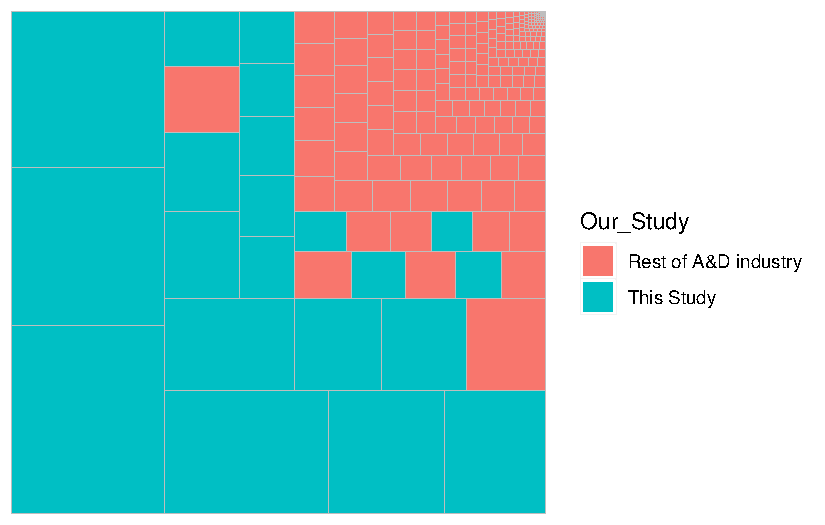
\includegraphics{defence_files/figure-pdf/fig-mktcapshare-1.pdf}

}

\caption{\label{fig-mktcapshare}Treemap of market capitalisation of our
study's sample}

\end{figure}

\hypertarget{references}{%
\section*{References}\label{references}}
\addcontentsline{toc}{section}{References}

\hypertarget{refs}{}
\begin{CSLReferences}{1}{0}
\leavevmode\vadjust pre{\hypertarget{ref-agapos1970}{}}%
Agapos, A. M., and Lowell E. Gallaway. 1970. {``Defense Profits and the
Renegotiation Board in the Aerospace Industry.''} \emph{Journal of
Political Economy} 78 (5): 1093--1105.
\url{https://doi.org/10.1086/259692}.

\leavevmode\vadjust pre{\hypertarget{ref-Ando.2022}{}}%
Ando, Tomohiro, Matthew Greenwood-Nimmo, and Yongcheol Shin. 2022.
{``{Quantile Connectedness: Modeling Tail Behavior in the Topology of
Financial Networks}.''} \emph{Management Science} 68 (4): 2401--31.
\url{https://doi.org/10.1287/mnsc.2021.3984}.

\leavevmode\vadjust pre{\hypertarget{ref-bohi1973}{}}%
Bohi, Douglas R. 1973. {``Profit Performance in the Defense Industry.''}
\emph{Journal of Political Economy} 81 (3): 721--28.
\url{https://doi.org/10.1086/260067}.

\leavevmode\vadjust pre{\hypertarget{ref-bu2019}{}}%
Bu, Hui, Wenjin Tang, and Junjie Wu. 2019. {``Time-Varying Comovement
and Changes of Comovement Structure in the Chinese Stock Market: A
Causal Network Method.''} \emph{Economic Modelling} 81 (September):
181--204. \url{https://doi.org/10.1016/j.econmod.2019.03.002}.

\leavevmode\vadjust pre{\hypertarget{ref-butler1966a}{}}%
Butler, Hartman L. 1966a. {``Aerospace Fundamentals and Industry
Analysis: Part I.''} \emph{Financial Analysts Journal} 22 (1): 55--60.
\url{https://doi.org/10.2469/faj.v22.n1.55}.

\leavevmode\vadjust pre{\hypertarget{ref-butler1966}{}}%
---------. 1966b. {``Aerospace Fundamentals and Industry Analysis: Part
II.''} \emph{Financial Analysts Journal} 22 (2): 41--48.
\url{https://doi.org/10.2469/faj.v22.n2.41}.

\leavevmode\vadjust pre{\hypertarget{ref-butler1967}{}}%
---------. 1967. {``Aerospace Industry Revisited.''} \emph{Financial
Analysts Journal} 23 (5): 57--62.
\url{https://doi.org/10.2469/faj.v23.n5.57}.

\leavevmode\vadjust pre{\hypertarget{ref-Cappelle.2008}{}}%
Capelle‐Blancard, Gunther, and Nicolas Couderc. 2008. {``{What drives
the market value of firms in the defense industry?}''} \emph{Review of
Financial Economics} 17 (1): 14--32.
\url{https://doi.org/10.1016/j.rfe.2007.02.001}.

\leavevmode\vadjust pre{\hypertarget{ref-Diebold.2009}{}}%
Diebold, Francis X., and Kamil Yilmaz. 2009. {``{Measuring Financial
Asset Return and Volatility Spillovers, with Application to Global
Equity Markets*}.''} \emph{The Economic Journal} 119 (534): 158--71.
\url{https://doi.org/10.1111/j.1468-0297.2008.02208.x}.

\leavevmode\vadjust pre{\hypertarget{ref-Diebold.2014}{}}%
Diebold, Francis X., and Kamil Yılmaz. 2014. {``{On the network topology
of variance decompositions: Measuring the connectedness of financial
firms}.''} \emph{Journal of Econometrics} 182 (1): 119--34.
\url{https://doi.org/10.1016/j.jeconom.2014.04.012}.

\leavevmode\vadjust pre{\hypertarget{ref-Dungey.2019}{}}%
Dungey, Mardi, John Harvey, and Vladimir Volkov. 2019. {``{The changing
international network of sovereign debt and financial institutions}.''}
\emph{Journal of International Financial Markets, Institutions and
Money} 60: 149--68. \url{https://doi.org/10.1016/j.intfin.2018.12.013}.

\leavevmode\vadjust pre{\hypertarget{ref-federle2022}{}}%
Federle, Jonathan, and Victor Sehn. 2022. {``Costs of Proximity to War
Zones: Stock Market Responses to the Russian Invasion of Ukraine.''}
\emph{SSRN Electronic Journal}.
\url{https://doi.org/10.2139/ssrn.4060222}.

\leavevmode\vadjust pre{\hypertarget{ref-huang2021}{}}%
Huang, Chuangxia, Yunke Deng, Xiaoguang Yang, Jinde Cao, and Xin Yang.
2021. {``A Network Perspective of Comovement and Structural Change:
Evidence from the Chinese Stock Market.''} \emph{International Review of
Financial Analysis} 76 (July): 101782.
\url{https://doi.org/10.1016/j.irfa.2021.101782}.

\leavevmode\vadjust pre{\hypertarget{ref-kumar2022}{}}%
Kumar, Ashish, Najaf Iqbal, Subrata Kumar Mitra, Ladislav Kristoufek,
and Elie Bouri. 2022. {``Connectedness Among Major Cryptocurrencies in
Standard Times and During the COVID-19 Outbreak.''} \emph{Journal of
International Financial Markets, Institutions and Money} 77 (March):
101523. \url{https://doi.org/10.1016/j.intfin.2022.101523}.

\leavevmode\vadjust pre{\hypertarget{ref-Londono.2019}{}}%
Londono, Juan M. 2019. {``{Bad bad contagion}.''} \emph{Journal of
Banking \& Finance} 108: 105652.
\url{https://doi.org/10.1016/j.jbankfin.2019.105652}.

\leavevmode\vadjust pre{\hypertarget{ref-mcdonald2011}{}}%
McDonald, James E., and Walter R. Kendall. 2011. {``Measuring the
Economic Effects of Political Events: War and the u.s. Defense
Industry.''} \emph{Journal of Applied Business Research (JABR)} 10 (1):
57. \url{https://doi.org/10.19030/jabr.v10i1.5963}.

\leavevmode\vadjust pre{\hypertarget{ref-suarez1976}{}}%
Suarez, James M. 1976. {``Profits and Performance of Aerospace Defense
Contractors.''} \emph{Journal of Economic Issues} 10 (2): 386--402.
\url{https://doi.org/10.1080/00213624.1976.11503352}.

\leavevmode\vadjust pre{\hypertarget{ref-valukonis2014}{}}%
Valukonis, Mantas. 2014. {``CHINA's STOCK MARKET TRENDS AND THEIR
DETERMINANTS ANALYSIS USING MARKET INDICES.''} \emph{ECONOMICS AND
MANAGEMENT} 18 (4). \url{https://doi.org/10.5755/j01.em.18.4.5096}.

\leavevmode\vadjust pre{\hypertarget{ref-zhang2022}{}}%
Zhang, Zhengyong, Elie Bouri, Tony Klein, and Naji Jalkh. 2022.
{``Geopolitical Risk and the Returns and Volatility of Global Defense
Companies: A New Race to Arms?''} \emph{International Review of
Financial Analysis} 83 (October): 102327.
\url{https://doi.org/10.1016/j.irfa.2022.102327}.

\end{CSLReferences}



\end{document}
